% -*- UTF-8 : LaTeX -*-
\documentclass[10pt,oneside,a4paper,titlepage]{article}

\usepackage[hangul,nonfrench,finemath]{kotex}
\usepackage[default]{dhucs-interword}
\usehangulfontspec{ut}
\usepackage[hangul]{dhucs-setspace}
\usepackage{dhucs-gremph}

\usepackage{listings}
\usepackage[all]{xy}
\usepackage{indentfirst}
\usepackage[dvips]{graphicx}
\usepackage{graphicx}
\usepackage{fullpage}
\usepackage{float}

\usepackage{color}
\definecolor{dkgreen}{rgb}{0,0.6,0}
\definecolor{gray}{rgb}{0.5,0.5,0.5}
\definecolor{mauve}{rgb}{0.58,0,0.82}

\usepackage{ifpdf}
\ifpdf
  \usepackage[unicode,pdftex,colorlinks]{hyperref}
  \input glyphtounicode\pdfgentounicode=1
\else
  \usepackage[unicode,dvipdfm,colorlinks]{hyperref}
\fi

\lstset{language=C++, 
numberstyle=\tiny\color{gray},
  keywordstyle=\color{blue},
  commentstyle=\color{dkgreen},
  stringstyle=\color{mauve},
  numbers=none,
  breaklines=true,showspaces=false,showstringspaces=false,
  morekeywords={slots,signals,emit},
  captionpos=b,framexleftmargin=10pt,frame=single
}
  
\renewcommand*\lstlistingname{소스 코드}
\renewcommand*\lstlistlistingname{소스 코드 차례}

\title{객체 조별 프로젝트 3조\\
BlueScreen}
\author{
ME   20110307 박진석 jinmel\\
CHEM 20100420 유찬미 ycm0830\\
CSED 20120425 김홍기 khg1004\\ 
CSED 20120188 김범수 kimbs45\\
CITE 20120321 박원표 parkwonpyo\\
MATH 20120002 이주현 trozlee\\
CSED 20080640 이상학 uzbu89
}

\begin{document}

\maketitle

\newpage

%명예서약
\begin{center}
{\Huge\textbf{명예서약}}
\end{center}

\begin{center}
{\Large\textbf{나는 이 프로그래밍 과제를 다른 사람의 부적절한 도움 없이 완수하였습니다.}}
\end{center}
\newpage

\tableofcontents
\listoffigures
\lstlistoflistings
\newpage

\section{개요}

\subsection{프로그램 주제 선정 배경}
최근에 가장 유행하는 게임 중에 하나가 '모두의 마블'이라는 게임이다. 이 게임은 2인 이상의 사용자가 게임 서버에 접속하여 그림 1과 같은 9개의 칸으로 구성된 4개의 line으로 이루어진 사각형의 게임 판에서 도시와 건물을 사고 팔면서 진행하는 게임이다. 우리 조는 이 게임을 떠올리며 게임을 진행하는 character, 각 도시를 상징하는 칸들, 주사위 등을 class에 적용하여 구현할 수 있지 않을까 생각하게 되었다. 이는 객체지향 프로그래밍에서 적합한 조건을 줄 수 있고 더불어 사용자들의 흥미도 끌 수 있기 때문이다. 
이 프로젝트를 통해 수업 시간에 배운 클래스, 상속, 다형성 등의 개념을 이용해 게임을 개발하여 OOP에 대한 이해도를 높이고 팀원들간의 협동심을 기르고자 한다. 
\subsection{프로그램 이름}
Postech Marble
\subsection{프로그램 기능}
이 프로그램은 Qt환경에서 object-oriented programming의 특성을 활용하여 개발한 Postech 버젼 ‘부루마블’ 게임이다.



\subsubsection{게임의 기능}
게임 시작, 주사위 굴리기, 과목 수강하기, 게임의 승리, 게임 종료

\subsubsection{게임 승리 조건}
한 학과의 모든 과목을 수강함과 동시에 모든 과목이 B 학점을 넘어야 한다. 만약 복수전공을 해야 할 상황일 경우 2개의 학과의 과목을 수강하고 일정 학점을 넘어야 된다.

\subsubsection{세부적인 게임 내용}

\begin{description}

\item[행동력] \hfill \\
기존 '모두의 마블'의 돈과 비슷한 개념이다. 과목을 수강하거나 다른 활동에 의해 소모된다. 

\item[과목] \hfill \\
맵의 한 라인에 2개의 학과가 있고 각각 3개씩 과목이 있다. 3개의 과목은 쉬운 과목, 보통 과목, 어려운 과목으로 나뉘어있다. 과목을 밟아서 수강할 경우 랜덤한 학점이 부여된다. 다른 사람이 그 과목을 밟을 경우 일정 활동력을 지불하며 원하는 경우 그 과목을 뺏어올 수도 있다. 과목의 학점을 낮게 받은 경우 재수강을 통해서 학점을 올릴 수도 있다. 게임에 존재하는 학과는 컴퓨터공학과, 수학과, 기계과, 화학과, 생명과, 산업경영공학과, 물리과, 전자과이다. 

\item[불금칸] \hfill \\
 각 라인에는 한 칸씩 술집이 있다. (설종빈, 통집). 불금 칸에 플레이어가 들어왔을 경우 일정 행동력을 잃는다.
\item[코너 칸] \hfill \\
보드에는 특별한 기능을 하는 총 4개의 코너 칸이 존재한다.
\begin{enumerate}
 \item 휴학: 휴학하여 이동할 수 없다. 하지만 자신의 차례에 더블이 나오면 탈출한다.
 \item 복수전공: 일정 확률로 복수전공을 하게 된다. 2개의 과목을 독점해야 된다.
 \item 61콜: 원하는 칸으로 갈 수 있다.
 \item 기숙사: starting point로서 여기를 지나면 일정한 활동력을 얻을 수 있다.
\end{enumerate}

\item[이벤트 블록칸] \hfill \\
롤, 술, 치킨, 과목 뺏기, CC, 과목 잃기 등의 활동을 통해서 행동력을 잃거나 얻을 수도 있고 그 외에 게임의 재미를 더하는 랜덤한 효과들이 있다.
\begin{enumerate}
\item Drink: 원하는 불금 칸으로 이동한다. 
\item CC: 50\%의 확률로 휴학, 50\%확률로 61콜로 이동한다.
\item TakeSubject: 상대방의 과목 중 하나를 가져올 수 있다.
\item LoseSubject: 과목을 하나 잃는다. 
\item LOL: 50\%의 확률로 행동력 50증가, 50\%의 확률로 100 감소
\item Chicken: 행동력 100상승
\item PhotoGenic: 조 사진 팝업.
\end{enumerate}


\item[캐릭터] \hfill \\
포스텍 마블에서는 다양한 캐릭터가 존재한다. 캐릭터는 게임이 시작될 때 랜덤하게 결정된다.
\begin{enumerate}
\item genius: 초기 행동력 1200
\item hard worker: 지급 행동력 150
\item lol gamer: event block의 lol 에서 언제나 승리.
\item Alcoholic: 불금에서 돈을 지불하지 않는다.r
\item Outsider: event block의 cc가 발동하지 않는다.
\end{enumerate}
\end{description}


\subsection{프로그램의 흐름}    
프로그램을 실행시킨 후, START 버튼을 클릭한다. 게임이 시작되면 각 플레이어의 캐릭터가 정해지고, 기숙사 칸에서 게임이 시작된다. 각각의 Turn마다 주사위를 2개 던져, 그 주사위 값의 합만큼 진행한다. 진행한 블록 위에 따라 행동을 정하고, 이는 게임의 승리조건을 만족할 때까지 반복한다. 게임의 승리조건은 플레이어가 한 학과의 과목을 독점하거나, 한 명의 플레이어를 제외한 나머지가 파산을 하여 게임을 진행할 수 없을 때, 두 가지다. 한 플레이어가 승리 조건을 만족하게 되면, 승리 문구와 함께 게임은 종료된다.

\section{프로그램 기능 설명}

\subsection{시작화면, 메인화면}

\begin{figure}[H]
\centerline{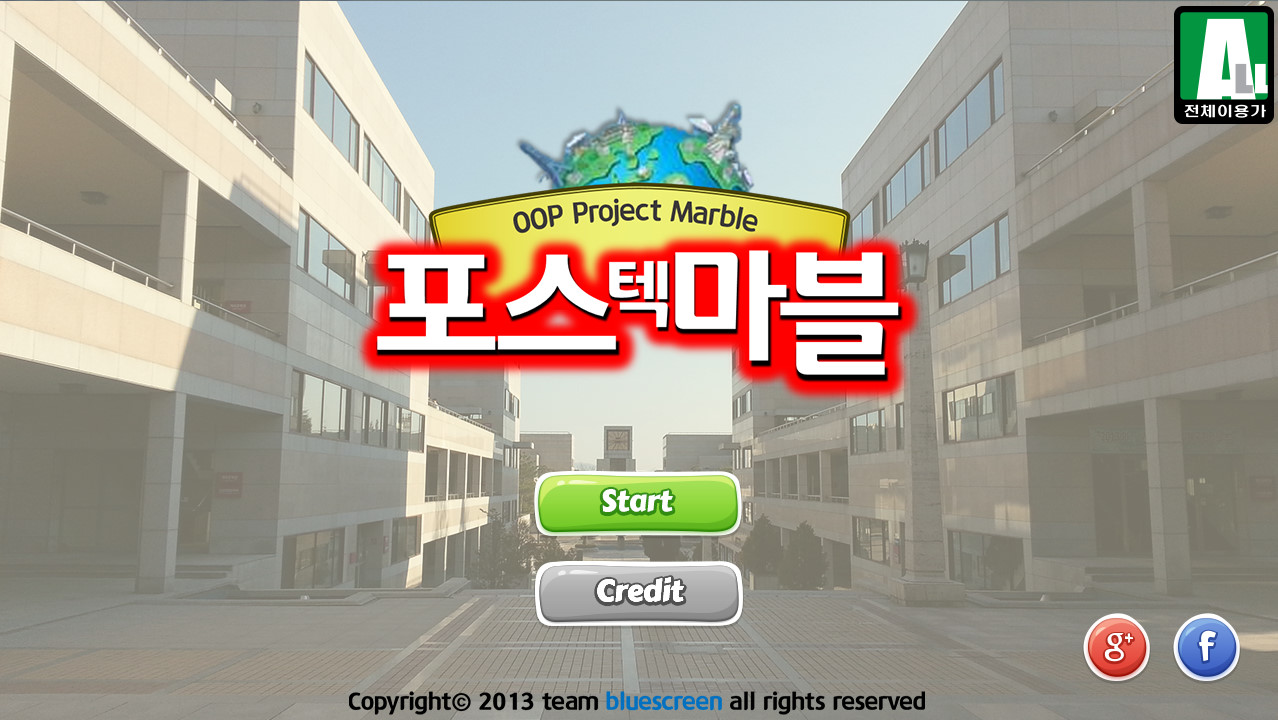
\includegraphics[scale=0.65]{images/1Main}}
\caption{메인화면}
\end{figure}

 게임을 실행하면 처음으로 블루스크린 팀의 로고가 나타난 뒤 메인 화면으로 진입한다. 메인화면에서 게임을 시작하거나 크레딧을 볼 수 있다. ‘모두의 마블’ 분위기가 나도록 이미지 리소스들을 사용하였고, $<$포스텍마블$>$이란 이름에 걸맞게 포스텍 캠퍼스를 배경으로 하고 있다.
 
 
\subsection{Credit}
\begin{figure}[H]
\centerline{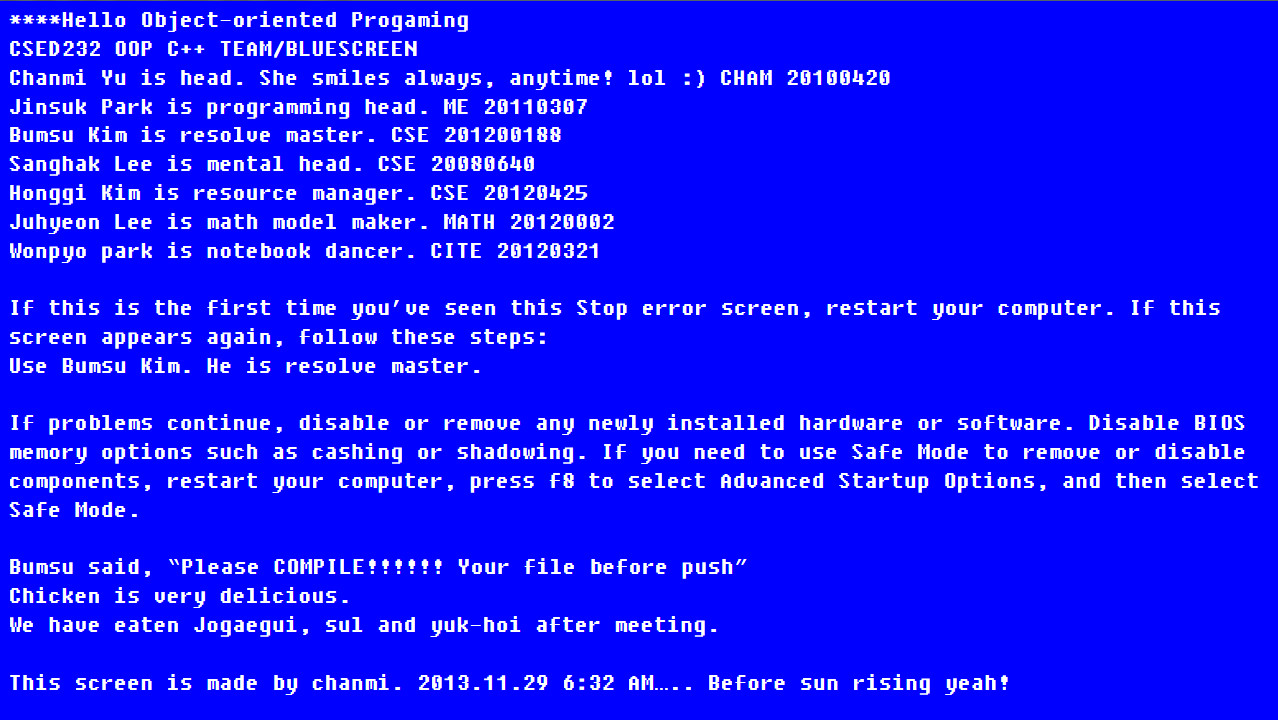
\includegraphics[scale=0.65]{images/2Credit}}
\caption{Credit}
\end{figure}

크레딧 화면은 게임의 메인 화면에서 들어가거나 게임의 승자가 결정된 후에 크레딧으로 진행되면서 접할 수 있는데, ‘Bluescreen’이라는 팀 명에 걸맞게 크레딧 화면의 컨셉을 블루스크린으로 잡았다. 크레딧 화면은 블루스크린 팀의 구성원과 각자의 역할을 설명하고 있다.

\subsection{캐릭터 선택}

\begin{figure}[H]
\centering
\centerline{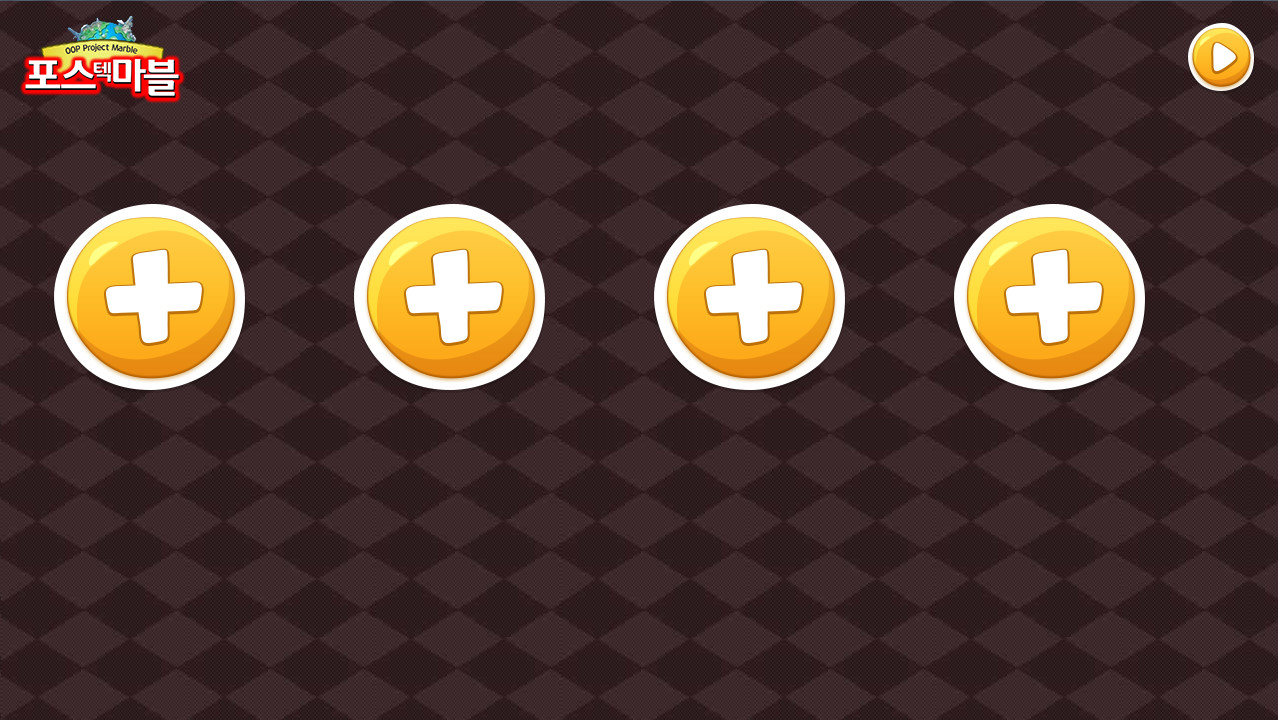
\includegraphics[scale=0.65]{images/3SelectCharacter}}
\caption{캐릭터 선택}
\end{figure}

\begin{figure}[H]
\centering
\centerline{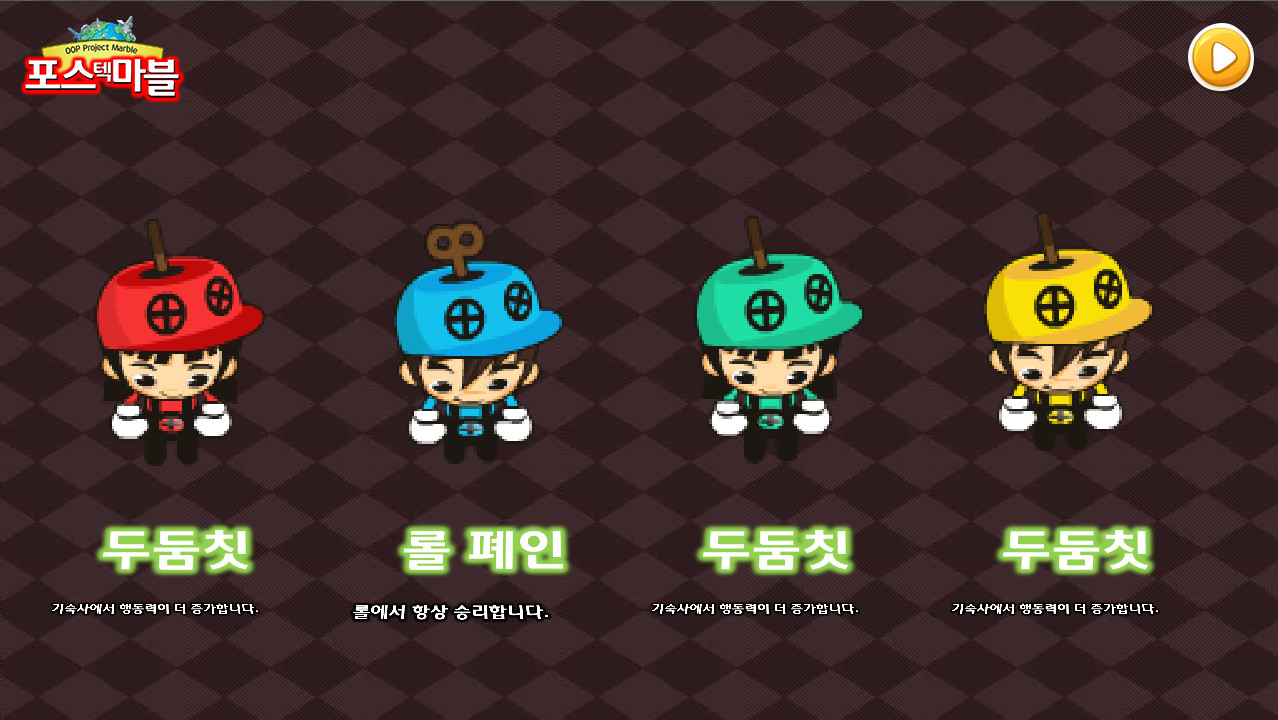
\includegraphics[scale=0.65]{images/3SelectCharacter2}}
\caption{캐릭터 선택}
\end{figure}
포스텍마블은 기본적으로 멀티플레이를 지원한다. 최소 2명부터 최대 4명까지 같이 게임을 플레이 할 수 있는데, +버튼을 누름으로서 플레이어의 수를 결정할 수 있다. +버튼을 누르는 순간 무작위로 캐릭터의 종류가 결정되며, 캐릭터 하단에 캐릭터 타입 이름과 그에 대한 설명이 있다. 캐릭터 타입으로는 똑똑이, 술꾼, 롤폐인, 아싸, 두둠칫 다섯 가지가 있으며, 다섯 캐릭터는 각각 다른 특성을 가진다. 같은 캐릭터 타입이 여러 번 나올 수 있으며, 한번 무작위로 지정된 캐릭터 타입은 바꿀 수 없다. 원하는 플레이어의 수를 결정한 뒤 재생 버튼을 누르면 보드 화면으로 넘어가면서 게임이 시작된다. 게임에서는 왼쪽에 있는 캐릭터부터 주사위를 굴리게 된다.


\subsection{게임 - 과목 수강}
\begin{figure}[H]
\centering
\centerline{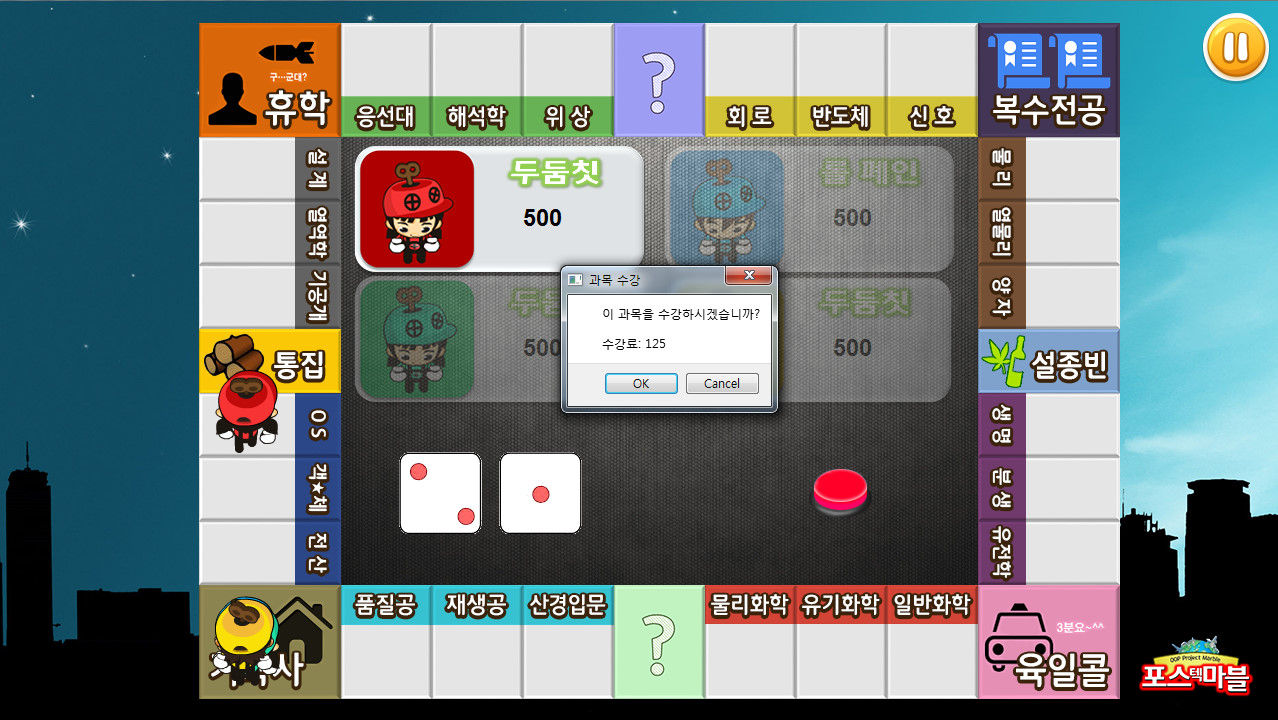
\includegraphics[scale=0.65]{images/4buySubject}}
\caption{과목 수강}
\end{figure}

 게임의 방식은 ‘모두의 마블’과 비슷한데, 주사위를 굴린 후 두 주사위의 눈의 합만큼 칸을 움직인 뒤, 칸의 종류에 따라 게임이 진행되는 방식이다. 칸의 종류로는 과목칸, 코너칸, 이벤트칸, 불금칸이 있는데, 가장 기본적이고 핵심적인 칸은 과목칸이라 할 수 있다. 과목칸은 8개의 과로 나눌 수 있으며, 한 플레이어가 과의 모든 과목들을 일정 학점 이상으로 (B학점) 수강하면 독점이 인정되는 구조로 게임이 진행된다. 일반적인 경우에는 한 과의 과목을 독점하면 게임에서 승리하게 된다. 다만 특수한 경우로는 코너 블록 ‘복수전공’에서 일정확률로 발동되는 복수전공에 해당되었을 경우 두 과의 모든 과목을 수강하는 경우에 승리할 수 있는데, 이 경우에는 각 과목들의 학점이 B이상이어야 한다는 제약이 해제된다. 각 블록마다 요구하는 행동력이 다르며, 번호가 늦은 (시계방향쪽으로 늦은) 블록의 필요 행동력이 더 높다. 과목 칸에 도달하면 팝업을 띄워 해당 과목을 수강할 지의 여부를 물어본다. 만약 수강을 원할 경우, 팝업에 표시된 수강료만큼의 행동력을 지불한 뒤, 해당 과목의 학점이 결정된다. 학점은 보드 위에 표시되며, 캐릭터와 겹치기 때문에 알아보기 어려운 면이 있지만, 학점을 표시하는 글자의 크기를 크게 하여 어느 정도 확인을 가능하게 하였다. 해당 과목을 어떤 플레이어가 소유하고 있는지 알아보기 위해서는 해당 칸에 표시된 학점의 색깔을 확인하면 된다.
 

\begin{figure}[H]
\centering
\centerline{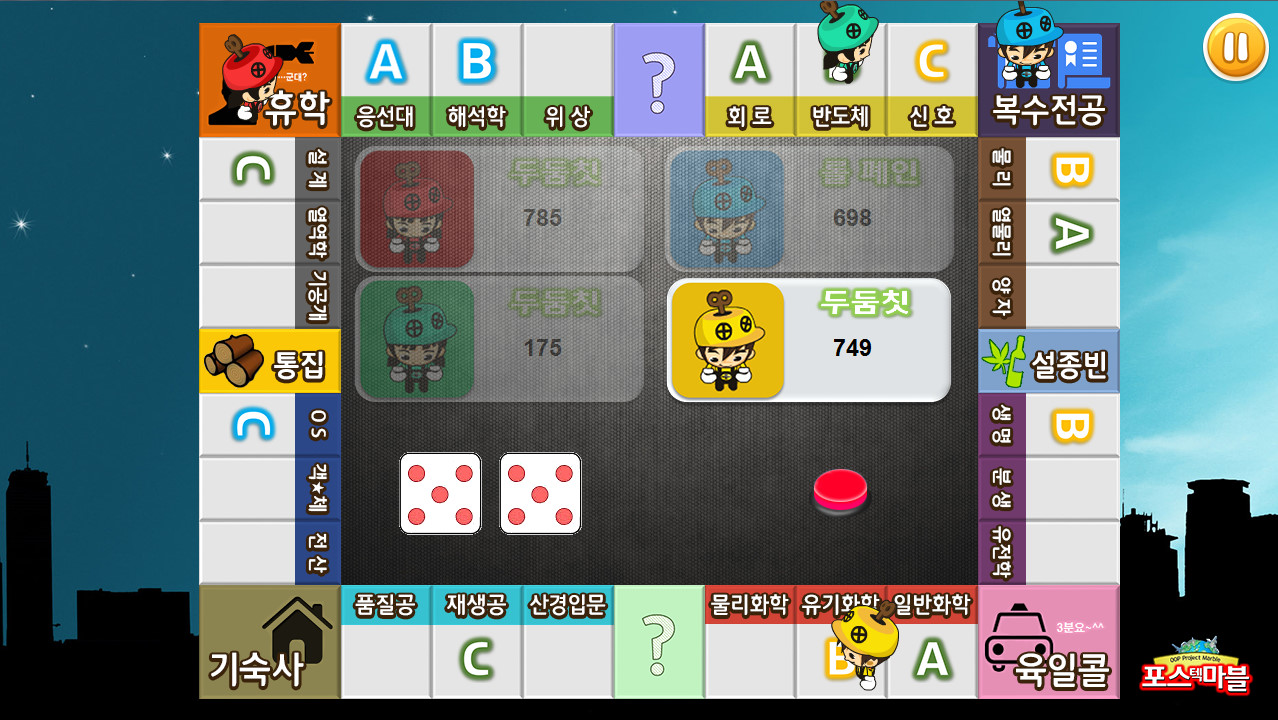
\includegraphics[scale=0.65]{images/4buySubject2}}
\caption{과목 수강}
\end{figure}
 
게임이 상당히 진행된 뒤의 보드. 여기서 ‘반도체’ 칸의 경우 캐릭터와 학점 글씨가 겹치기 때문에 알아보기 힘들 수 있지만, A, B, C 글자의 모양이 확연히 다르기 때문에 학점을 구분할 수 있다.
 
 
\subsection{게임 - 과목 인수}
\begin{figure}[H]
\centering
\centerline{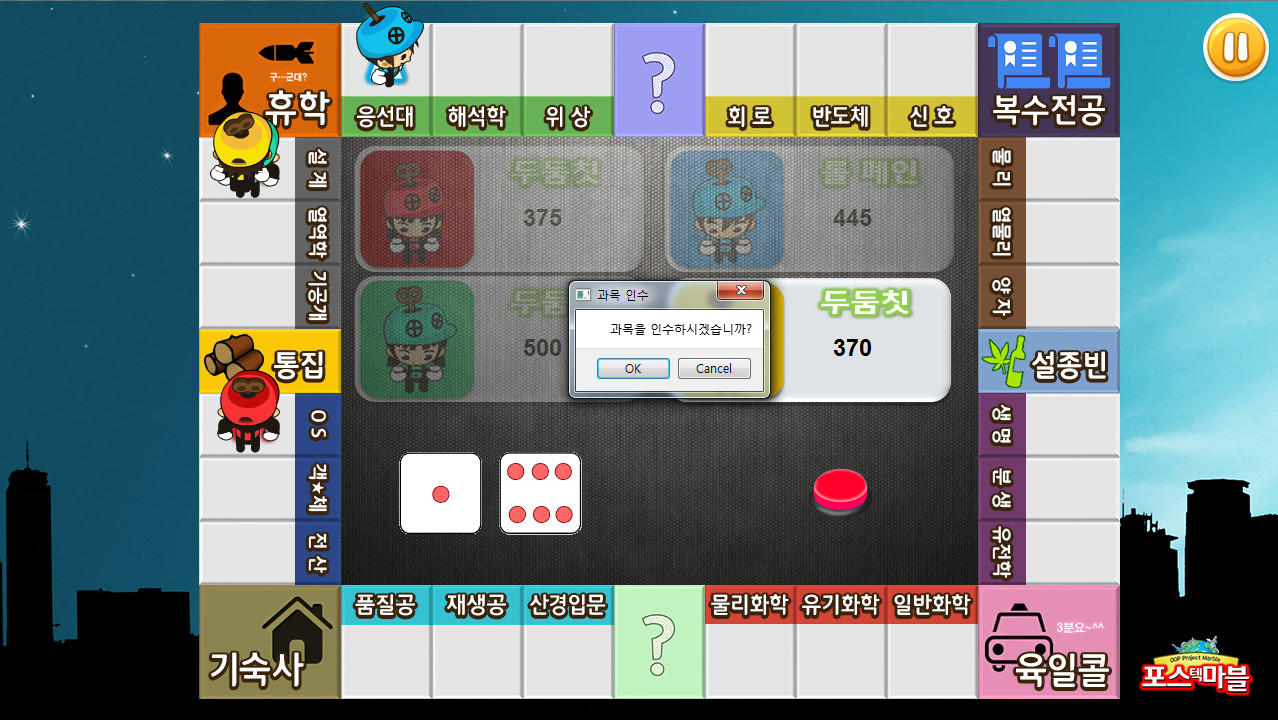
\includegraphics[scale=0.65]{images/5takeover}}
\caption{과목 인수}
\end{figure}

기본적으로 다른 사람이 소유하고 있는 과목의 칸에 도달하면 일정량의 행동력을 그 과목 칸을 소유하고 있는 플레이어에게 지불하여야 한다. 만약 다른 플레이어가 소유하고 잇는 칸에 도달한 플레이어가 행동력을 충분히 보유하고 있다면, 행동력을 지불한다. 행동력을 지불한 뒤에도 충분한 양의 행동력을 가지고 있으면, 그 과목 칸을 인수할 지의 여부를 팝업으로 띄워 물어본다. 플레이어가 인수 의사를 가지고 있다면, 행동력을 과목 칸을 소유한 플레이어에게 지급하고 그 칸을 자신의 소유로 한다. 인수 후에는 다시 무작위로 해당 과목의 학점이 결정되며, 오를 수도 있고 떨어질 수도 있다. 위의 스크린샷의 경우에는 status창이 밝게 되어있는 노란색 ‘두둠칫’ 캐릭터의 턴인데, 설계 과목 칸에 도달한 경우이다. 이 경우 충분한 양의 행동력을 가지고 있기 때문에 팝업을 띄워 인수 여부를 물어본다.	
 
\begin{figure}[H]
\centering
\centerline{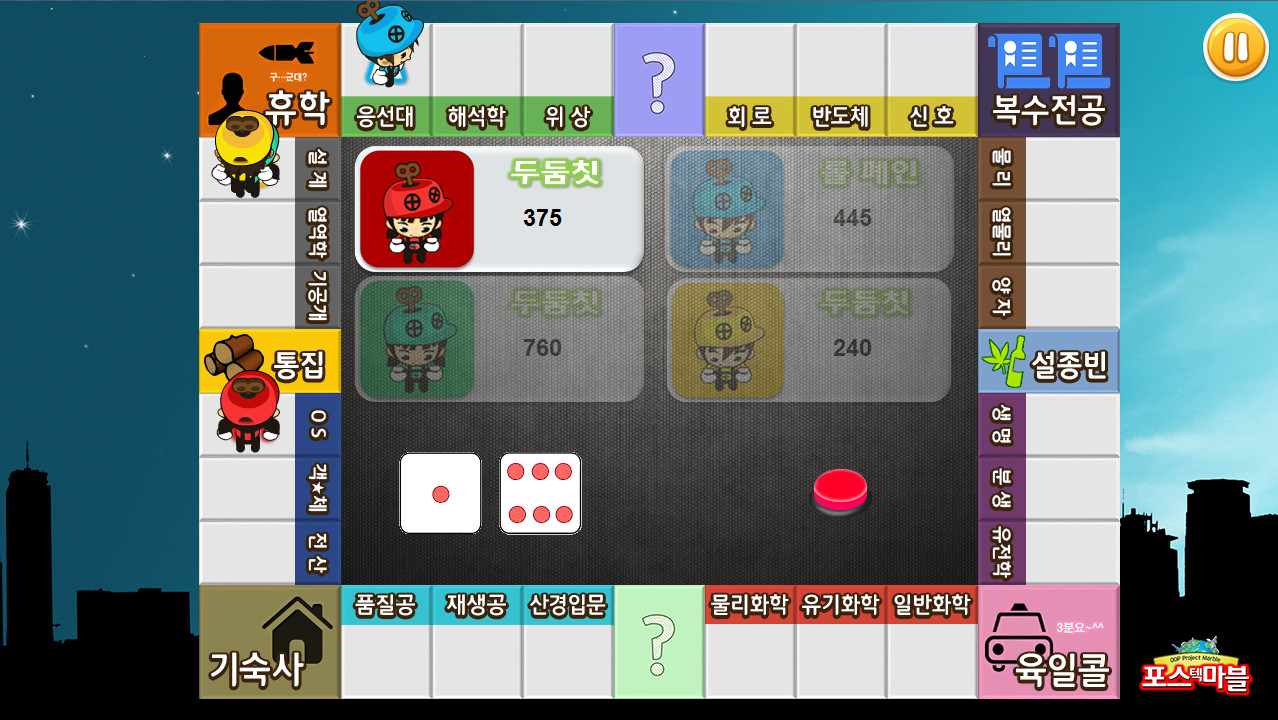
\includegraphics[scale=0.65]{images/5takeover2}}
\caption{과목 인수}
\end{figure}
 
 
여기서 노란색 ‘두둠칫’ 플레이어는 과목 칸을 인수하는 것을 선택했다. 이 경우 해당 칸의 학점이 재조정되며, 노란색 ‘두둠칫’ 플레이어의 행동력이 줄어들고 본래 과목 칸의 주인이었던 초록색 ‘두둠칫’ 플레이어의 행동력이 증가하였음을 확인할 수 있다.
 
\subsection{게임 - 수강 포기}

\begin{figure}[H]
\centering
\centerline{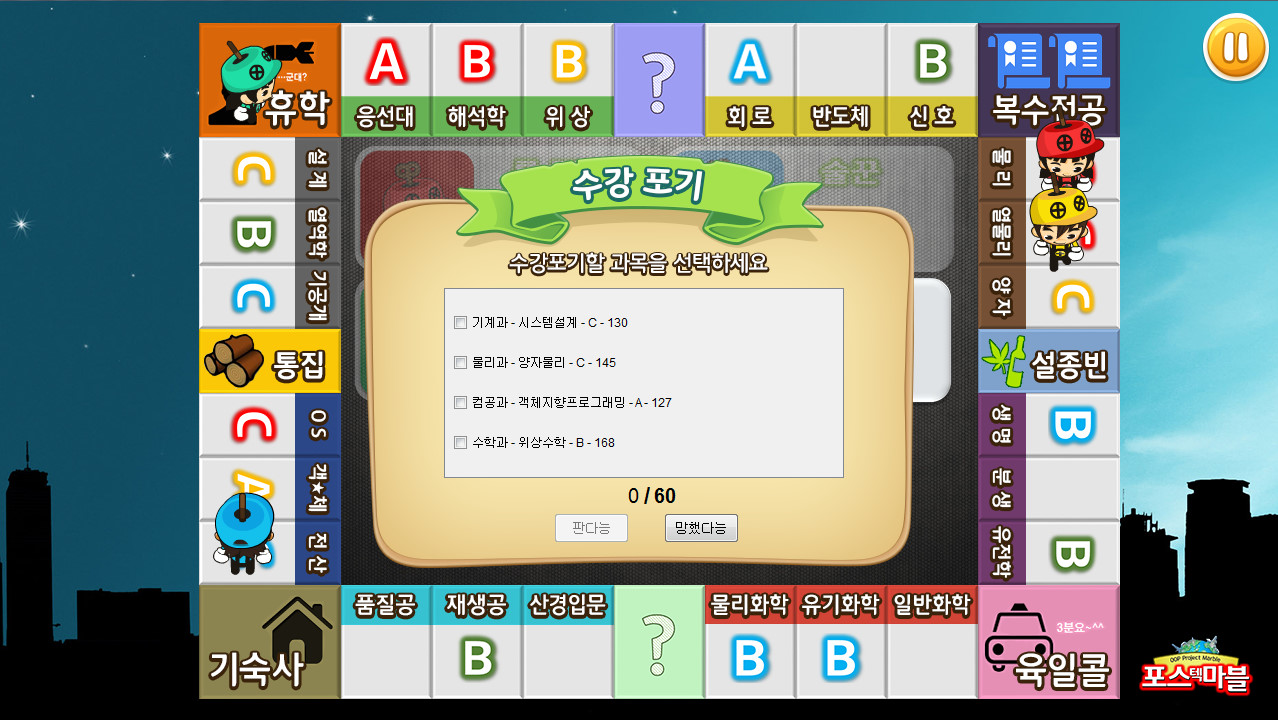
\includegraphics[scale=0.65]{images/6drop}}
\caption{과목 포기}
\end{figure}


 플레이어가 다른 플레이어가 소유한 과목 칸에 도달하였을 경우, 일정 행동력을 지불해야 한다. 하지만 해당 플레이어의 소유 행동력이 부족하면, 자신이 소유하고 있던 과목을 매각함으로서 지불해야 할 행동력을 마련해야 한다. 모든 과목을 매각해도 지불해야 할 행동력을 갖추지 못하면 플레이어는 자동으로 파산하게 된다. 포스텍마블에서는 이러한 매각 과정을 수강포기라고 부르는데, 수강포기를 해야 할 경우에는 팝업을 띄우면서 자신이 현재 소유하고 있는 과목과 해당 과목의 학점, 그리고 매각할 시 받을 수 있는 행동력, 마련해야 할 행동력을 표시하고 있다. 체크박스를 체크/해제 함으로서 해당 과목을 포기할 것인지의 여부를 판단할 수 있으며, 아래의 숫자를 통해 수강 포기로 행동력을 충분히 마련했는지 확인할 수 있다. 충분한 행동력을 마련한 경우 ‘판다능’ 버튼을 클릭하여 수강 포기를 완료할 수 있지만, 게임을 계속할 의지가 없는 경우에는 ‘망했다능’ 버튼을 눌러서 게임을 기권할 수 있다. 수강 포기한 과목은 주인이 사라지게 되며, 학점이 지워지게 된다.
 
\subsection{게임 - 재수강}

\begin{figure}[H]
\centering
\centerline{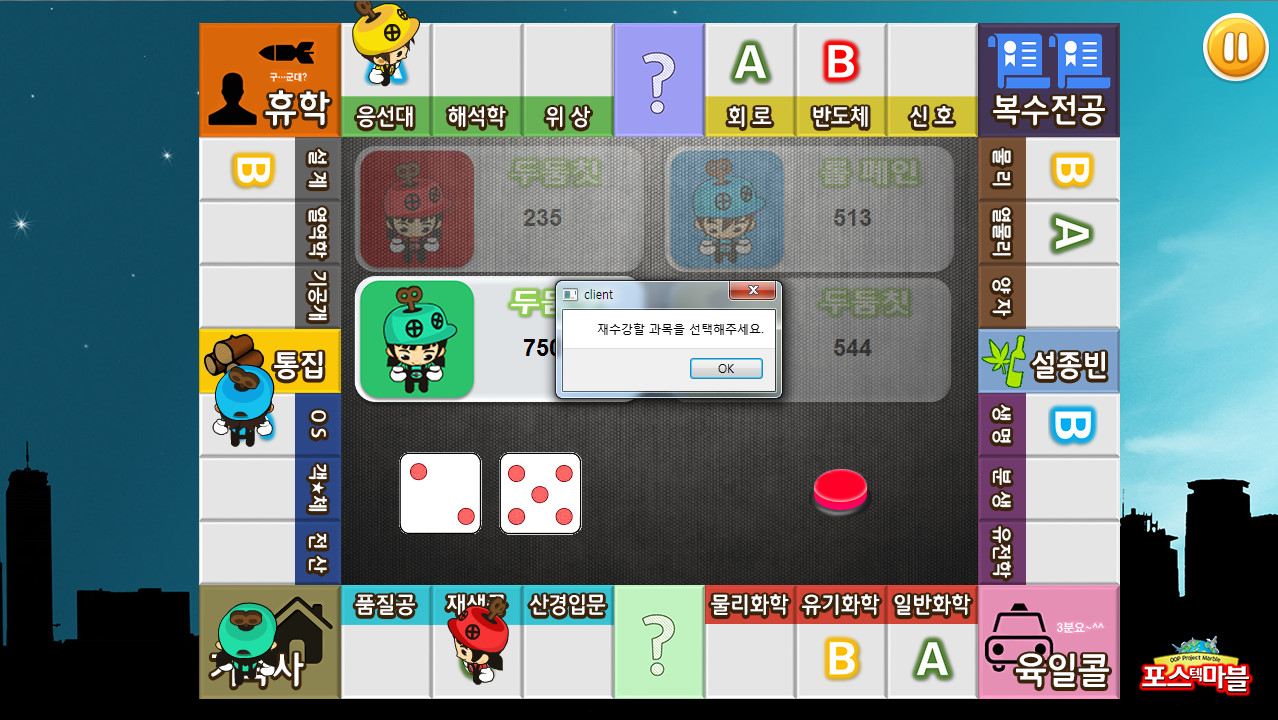
\includegraphics[scale=0.65]{images/7retake}}
\caption{과목 재수강}
\end{figure}

재수강은 크게 두 가지 방법으로 할 수 있는데, 첫 번째 방법은 자신이 소유하고 있는 과목 블록에 다시 도달하는 것이고, 다른 한 가지 방법은 코너 블록인 기숙사의 효과인 ‘원하는 과목 재수강’을 이용하여 재수강하는 경우이다. 자신이 소유하고 있는 과목 블록에 도달하는 경우는 팝업을 띄워 재수강 여부를 물어본다. 재수강의 경우는 학점이 무조건 올라가는 것이 아니며, 내려갈 수도 있기 때문에 전략적으로 재수강을 하지 않을 수도 있다. 기숙사 칸에 도달하는 경우는 재수강할 과목 하나를 선택하여 그 과목을 재수강할 수 있다. 재수강의 경우는 추가로 행동력을 지불하지 않고, 학점을 바꿀 수 있기 때문에 과목 독점, 통행료 상승을 목적으로 이용될 수 있다.
 
\subsection{게임 - 코너칸}
\begin{figure}[H]
\centering
\centerline{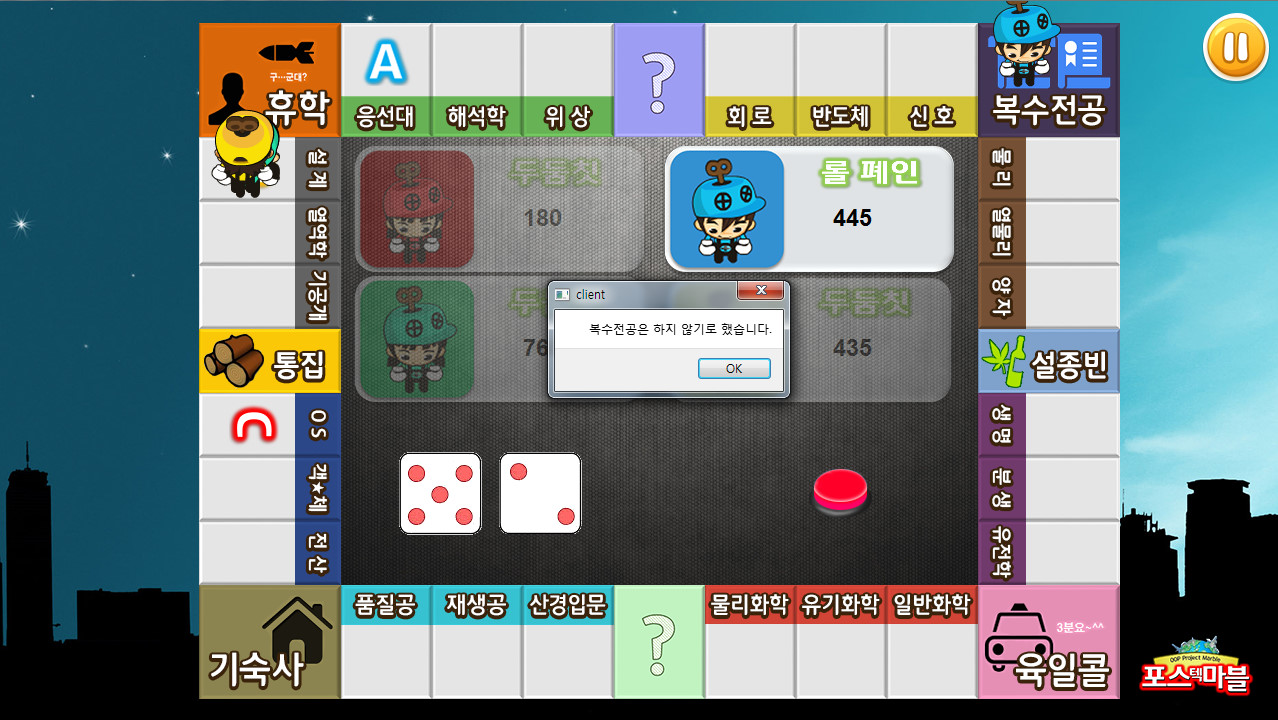
\includegraphics[scale=0.65]{images/8corner1}}
\caption{게임 코너칸}
\end{figure}
\begin{figure}[H]
\centering
\centerline{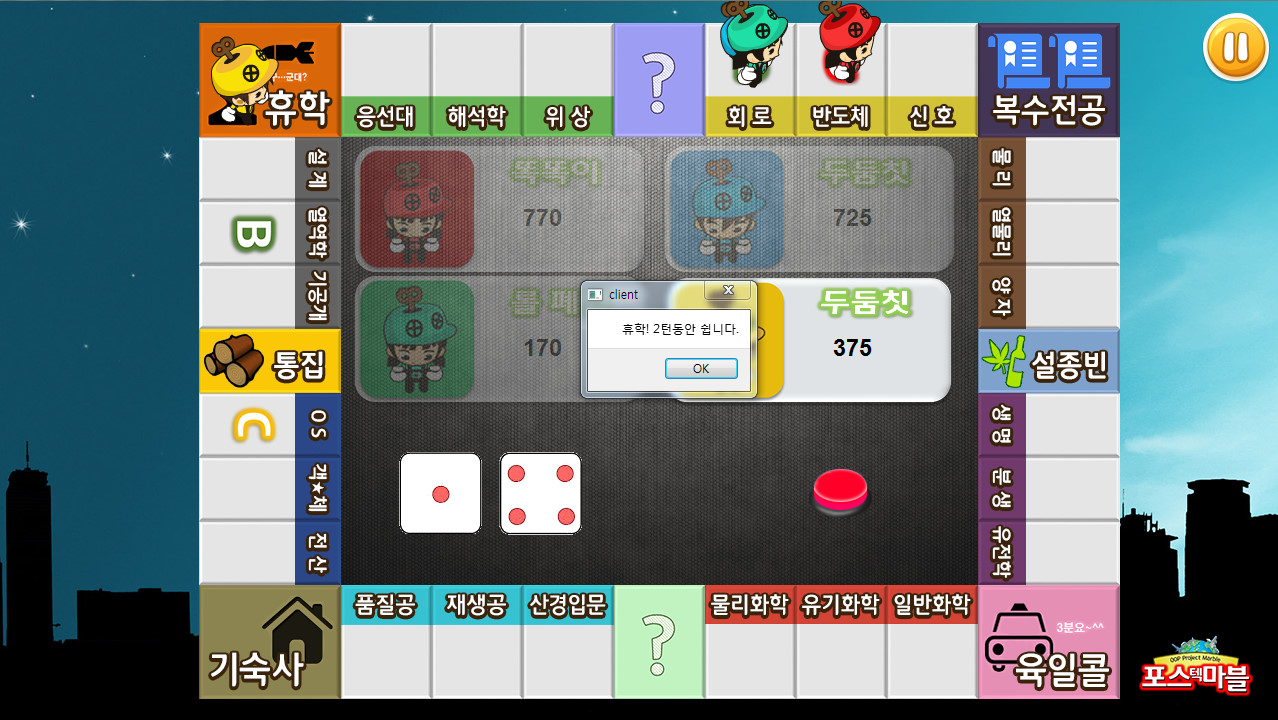
\includegraphics[scale=0.65]{images/8corner2}}
\caption{게임 코너칸}
\end{figure}
\begin{figure}[H]
\centering
\centerline{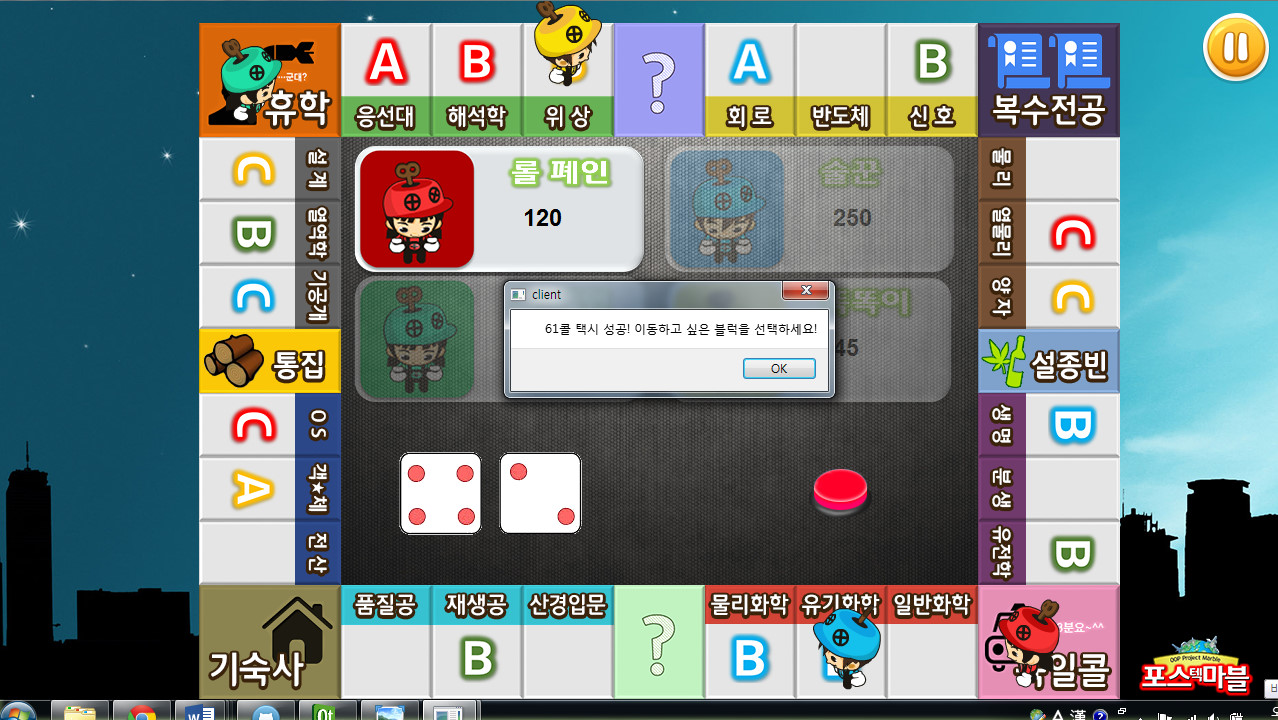
\includegraphics[scale=0.65]{images/8corner3}}
\caption{게임 코너칸}
\end{figure}



코너 블록은 대각선 방향 모퉁이에 있는 네 칸을 말하며, 기숙사, 휴학, 복수전공, 61콜 네 가지가 있다. 이 중 기숙사의 경우는 재수강에서 설명하였으므로 생략한다. 
휴학의 경우는 ‘모두의 마블’에서의 무인도와 같은 개념으로 휴학 칸에 도달할 경우 두 턴 동안 쉬어야 한다. 다만 탈출 방법이 있는데, 그 방법은 주사위가 더블이 나오는 것이다. ‘모두의 마블’과는 달리 포스텍마블에서는 행동력을 지불함으로써 휴학 칸을 탈출할 수 없다. ‘모두의 마블’과는 달리 이 게임에서는 턴 제한이 없기 때문에 피하는 것이 좋은 블록이라 할 수 있다.
복수전공 블록은 일정 확률로 복수전공 칸에 도달한 플레이어를 ‘복수전공’ 상태로 만들게 하는데, 복수전공 상태에서는 두 과의 과목을 모두 수강해야 승리 조건으로 인정된다. 다만 이 경우에는 패널티가 크기 때문에, 독점의 다른 조건인 ‘과의 모든 과목 학점 B이상’이라는 조건을 해제하여 준다.
61콜 블록은 ‘모두의 마블’에서의 세계일주와 비슷한 개념인데, 다른 점은 ‘모두의 마블’의 경우는 일정 금액을 지불하고 자신이 원하는 칸을 가는 방식인데 비하여, 포스텍마블에서는 일정 확률로 통행료를 내지 않고 자신이 원하는 칸으로 가는 방식이다. 모두의 마블과는 달리 자신이 원하는 칸으로 가는 경우 그 경로가 기숙사를 지난다 해도 기숙사에서 받는 행동력을 받을 수 없다는 단점이 있다. 복수전공이 아닌 경우에는 한 과의 세 과목을 들으면 승리 조건을 충족시키기 때문에 자신이 원하는 칸으로 간다는 것은 게임을 끝내거나 상당히 유리한 고지를 점할 수 있게 한다.

\subsection{게임 - 이벤트}

\begin{figure}[H]
\centering
\centerline{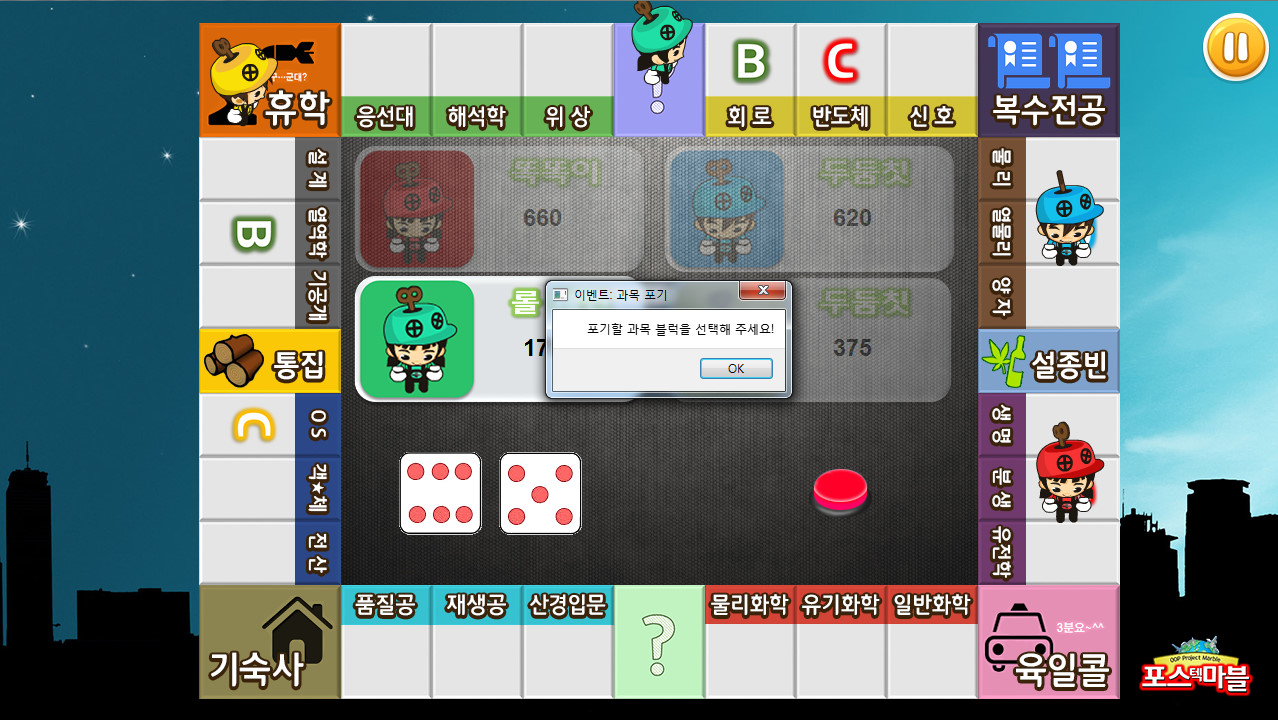
\includegraphics[scale=0.65]{images/9event1}}
\caption{게임 이벤트}
\end{figure}

\begin{figure}[H]
\centering
\centerline{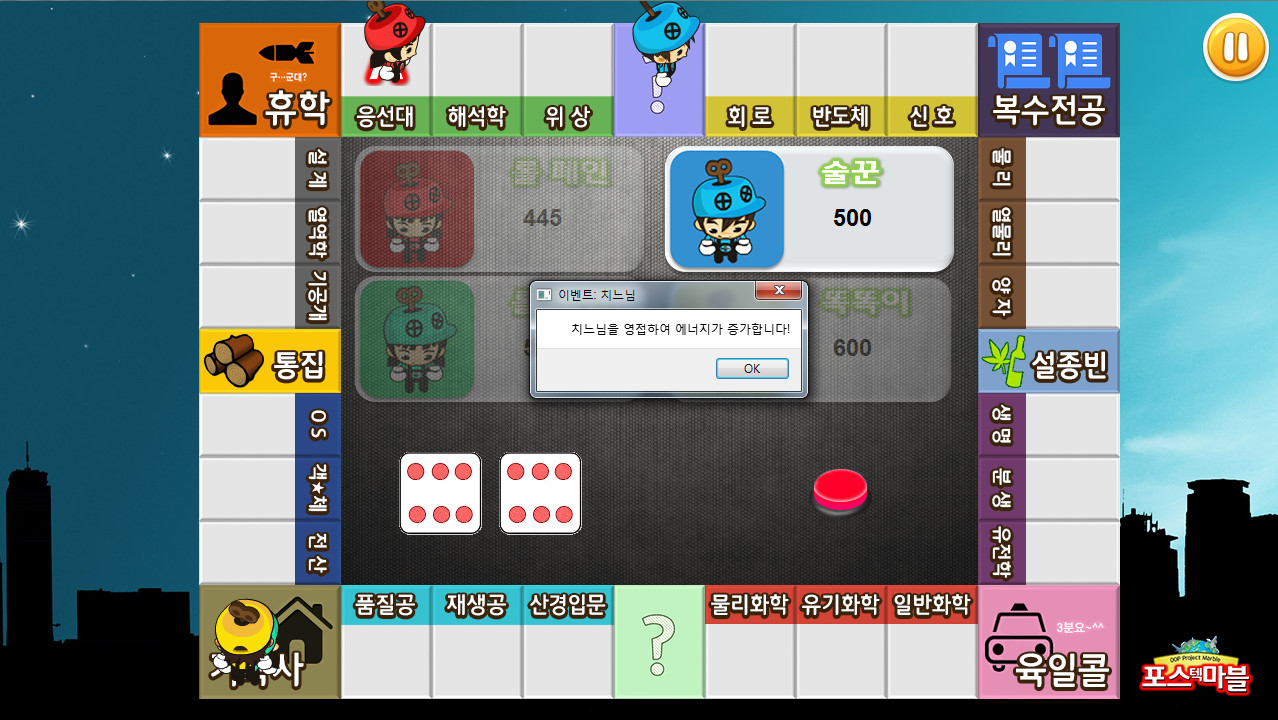
\includegraphics[scale=0.65]{images/9event2}}
\caption{게임 이벤트}
\end{figure}

\begin{figure}[H]
\centering
\centerline{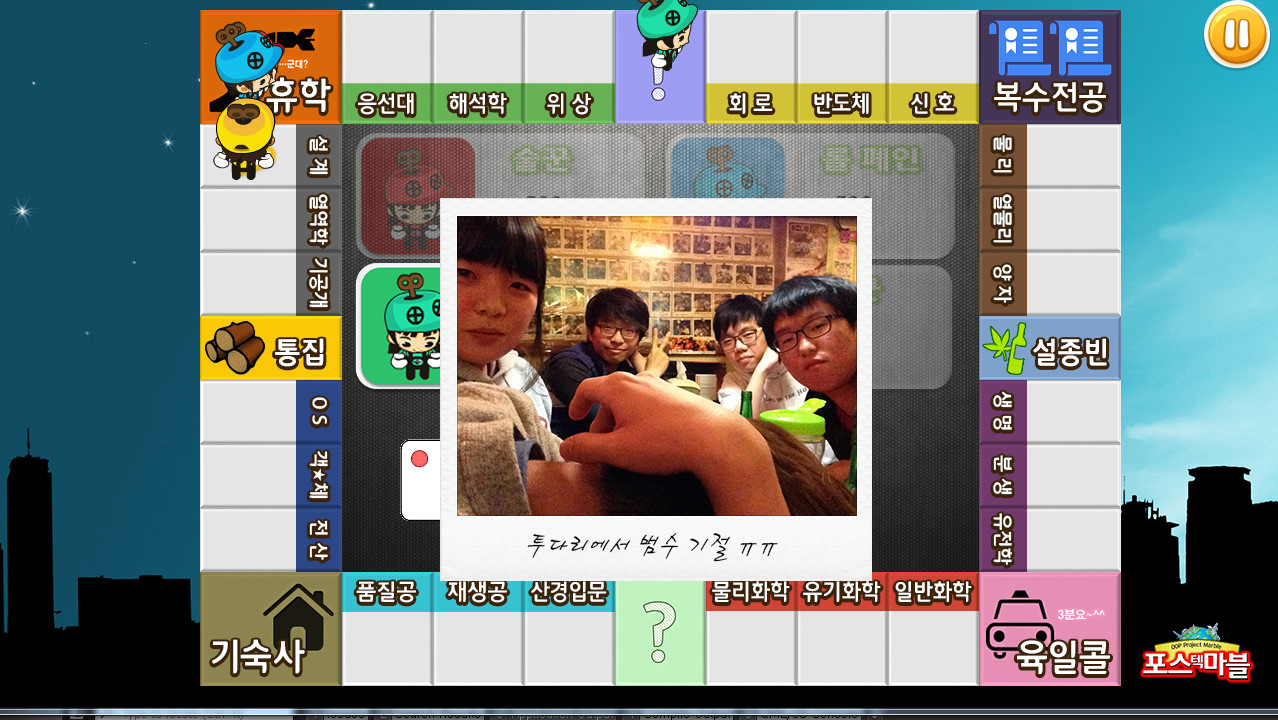
\includegraphics[scale=0.65]{images/9event3}}
\caption{게임 이벤트}
\end{figure}

\begin{figure}[H]
\centering
\centerline{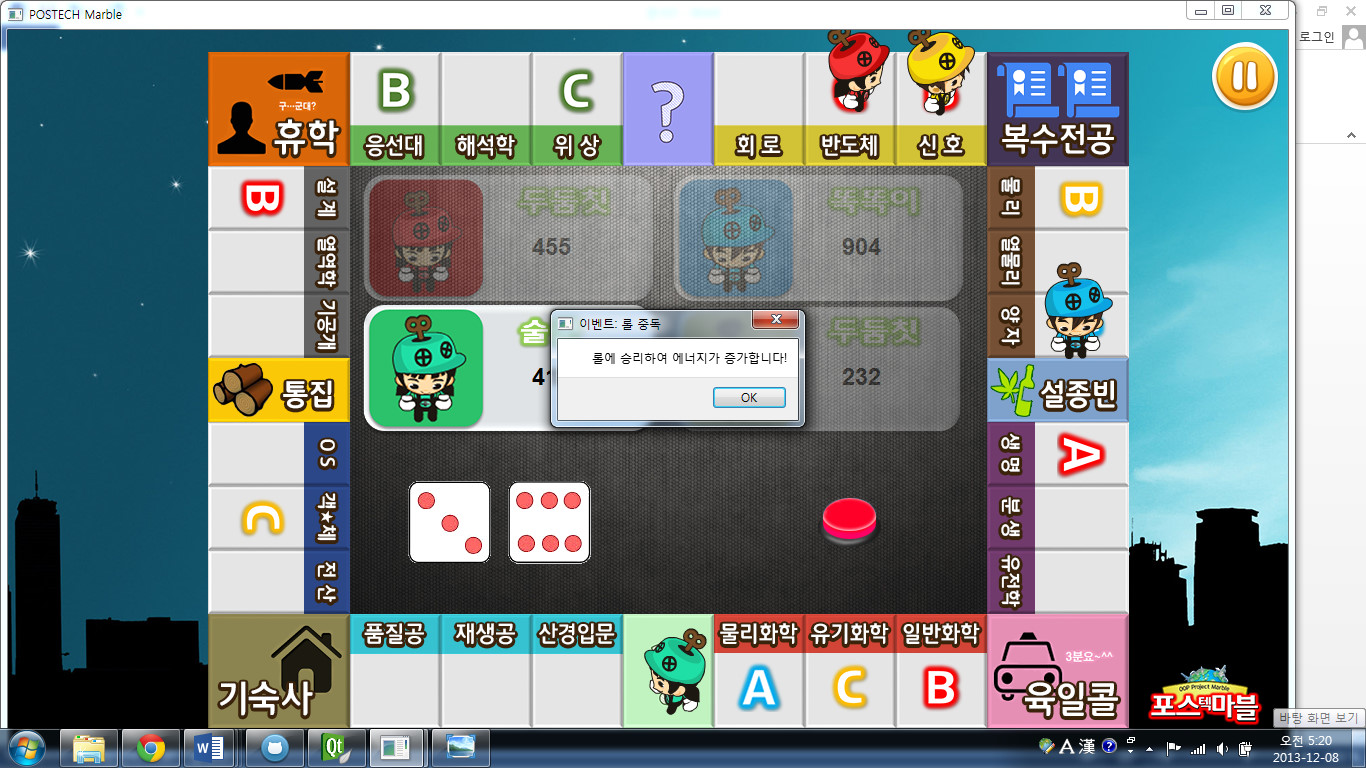
\includegraphics[scale=0.65]{images/9event4}}
\caption{게임 이벤트}
\end{figure}

이벤트 칸은 가로 줄의 ‘?’ 표시가 되어 있는 칸으로, 이벤트 간에 도착하면 무작위로 특정한 이벤트가 일어나게 된다. 첫 번째 스크린샷의 경우는 한 과목을 강제로 팔아야 하는 이벤트로, 자신이 가지고 있는 과목 중 하나를 포기해야 한다. 반대로 자신이 원하는 한 과목을 수강하는 이벤트도 있으며, 이 경우에는 아무도 수강하지 않은 과목을 선택해야 한다는 제한이 있다. 두 번째 스크린샷의 경우는 행동력이 증가하는 경우이며, 일정량의 행동력을 지급한다. 세 번째 스크린샷은 특별 이벤트인 ‘포토제닉’이며, 플레이어에게 영향을 미치지는 않지만 개발 중에 찍었던 사진 중 랜덤한 세 개를 보여주며 게임 플레이 도중 색다른 재미를 준다. 네 번째 스크린샷은 롤을 플레이 하는 경우인데, 확률적으로 롤에 승리하거나 패배한다. 롤에 승리한 경우는 소량의 행동력을 획득하며, 패배한 경우는 승리하였을 때 받는 행동력보다 더 많은 양의 행동력을 잃게 된다. 다만 롤 폐인 캐릭터의 경우는 롤에서 항상 승리하게 되어, 롤 이벤트가 발동하는 경우는 항상 행동력을 획득한다.
 
\subsection{게임 - 불금칸}
\begin{figure}[H]
\centering
\centerline{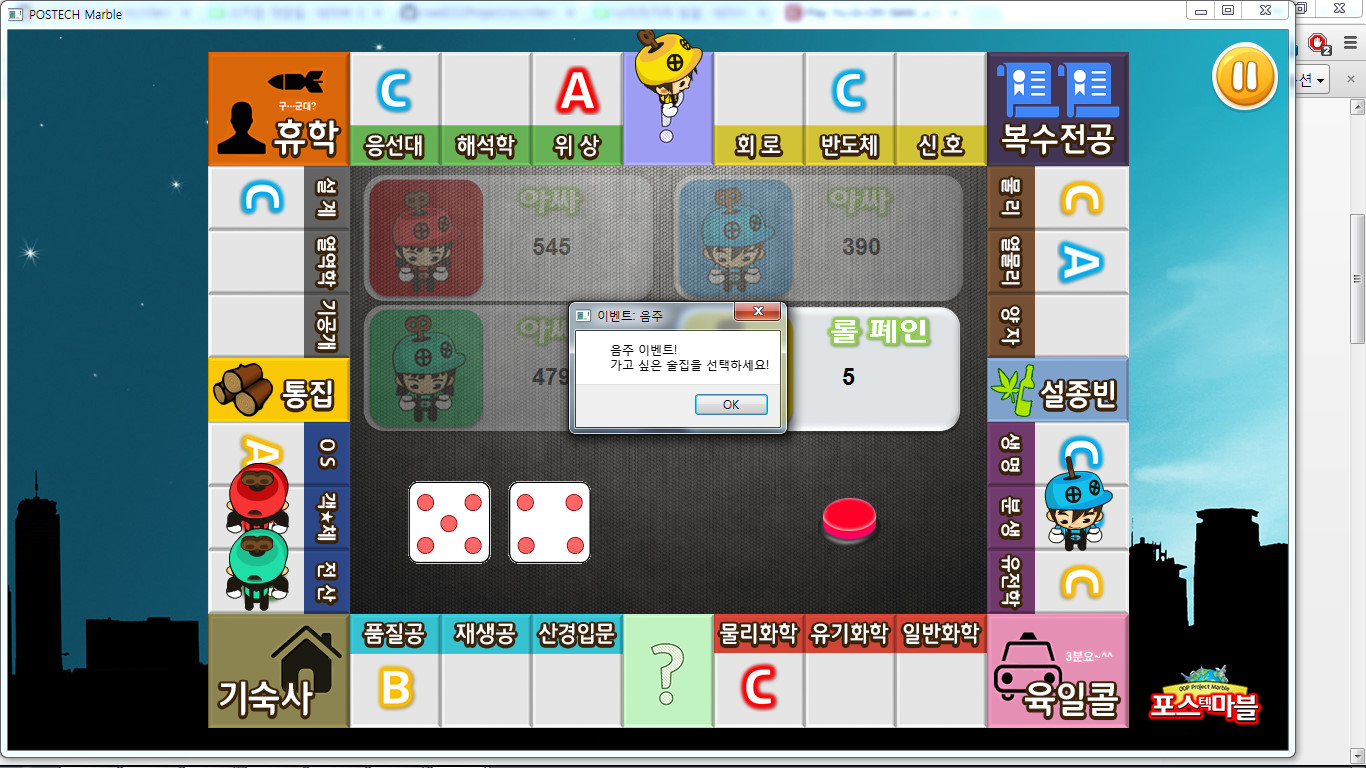
\includegraphics[scale=0.65]{images/10firefriday}}
\caption{게임 불금칸}
\end{figure}

\begin{figure}[H]
\centering
\centerline{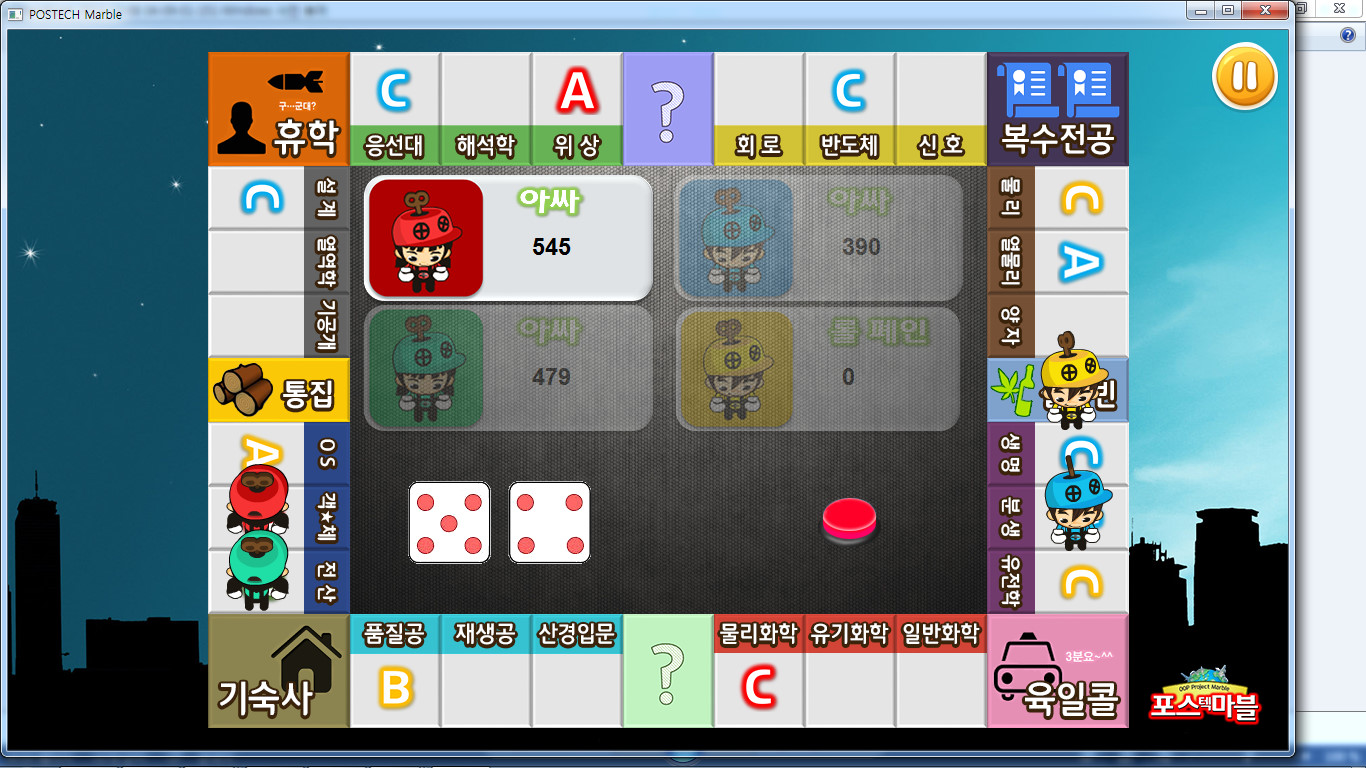
\includegraphics[scale=0.65]{images/10firefriday2}}
\caption{게임 불금칸}
\end{figure}


 불금 칸은 포스텍 주변의 술집을 모티브로 한 칸으로, ‘통집’과 ‘설종빈’ 두 개의 칸이 있다. 이 칸에 진입하는 경우는 행동력을 지불하는데, 술꾼 캐릭터일 경우는 다른 캐릭터와는 달리 불금 칸에 진입 한 경우 행동력을 획득한다는 차이가 있다. 두 칸의 기능은 동일하고, 이벤트 칸에서 ‘음주’ 이벤트가 발동하는 경우 자신이 원하는 불금 칸으로 이동할 수 있는 이벤트가 존재한다.
 
\subsection{게임 - 승리}


\begin{figure}[H]
\centering
\centerline{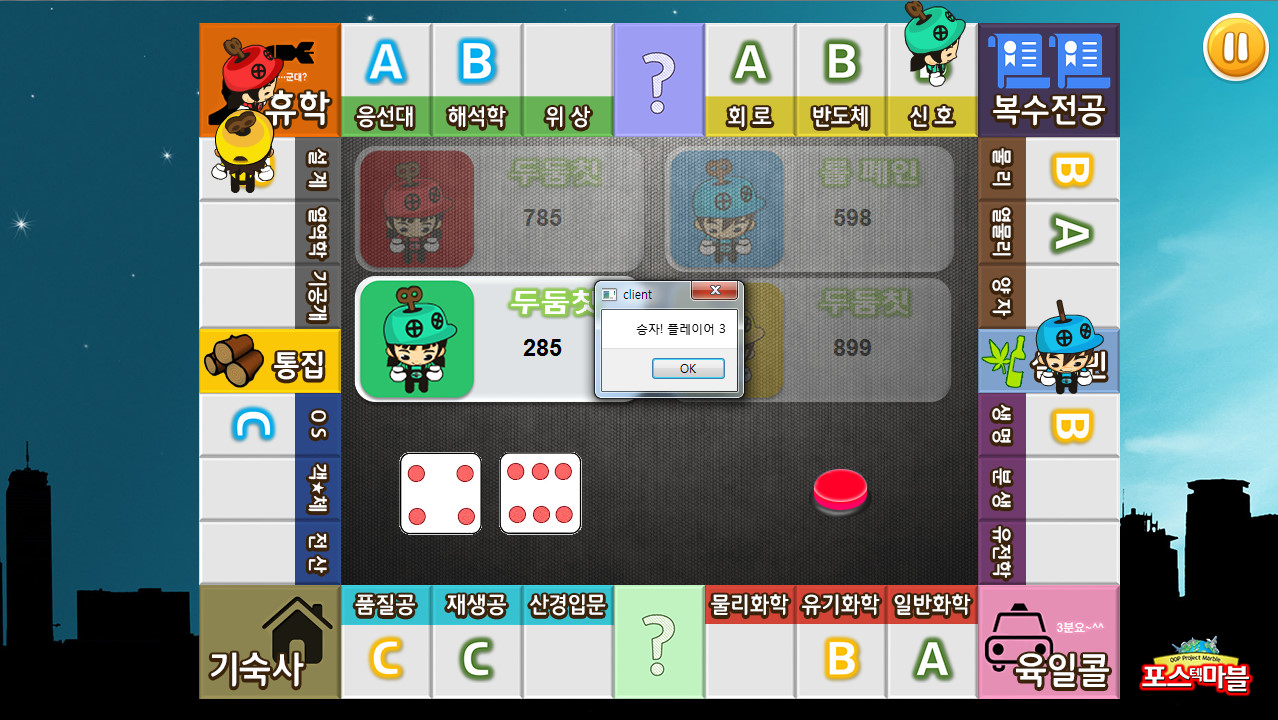
\includegraphics[scale=0.65]{images/11winner}}
\caption{게임 승리}
\end{figure}

\begin{figure}[H]
\centering
\centerline{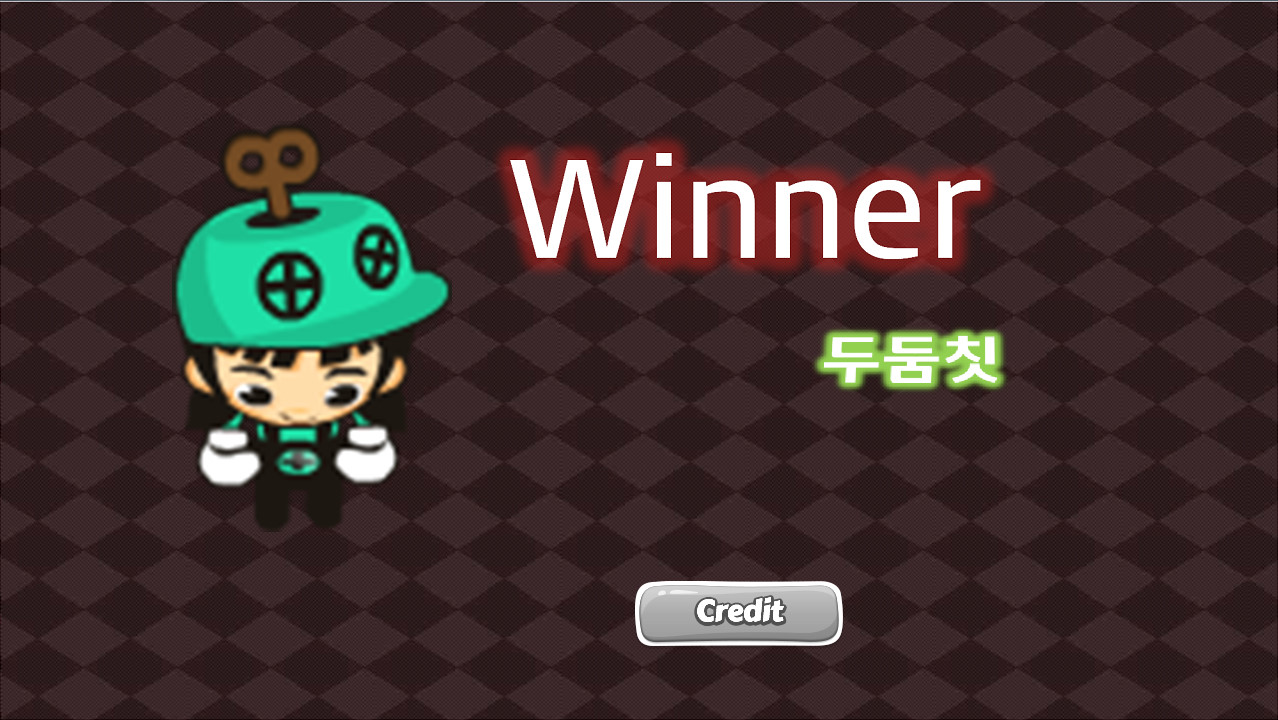
\includegraphics[scale=0.65]{images/11winner2}}
\caption{게임 승리}
\end{figure}

 일반적인 경우는 한 과의 과목을 B학점 이상으로 모두 수강, 복수전공의 경우는 두 과의 모든 과목을 수강, 또는 자신을 제외한 모든 플레이어가 파산하는 경우 승자가 된다. 승자가 결정된 경우는 팝업으로 어떤 플레이어가 승리하였는지 알리고, 승자를 표시하는 화면을 표시한다. 마지막으로, 크레딧 화면을 띄운 뒤, 다시 메인 화면으로 돌아가는 것으로 게임을 완전히 끝내게 된다.

 

\section{프로그램 소스 분석}

\subsection{Qt 프레임워크 활용}

\subsubsection{QGraphics Framework}
게임을 만들기 위해서 QGraphics Framework를 활용하였다. 이는 Qt에서 그래픽 출력을 담당하는 가장 기본적인 프레임워크이다. QGraphics 프레임워크는 QGraphicsView, QGraphicsScene, QGraphicsItem의 상호작용으로 이루어진다. 

\begin{description}
\item[QGraphicsView] \hfill \\
Qt 그래픽스를 말 그대로 보여주는(view) 클래스이다. Scene을 보여주는 창을 제공하며, 프로그램에서 실행 창을 담당하며, 실행 창의 내용은 그것의 scene이 담당하게 된다. 
\item[QGraphicsScene] \hfill \\
QGraphicsView가 보여줄 장면(Scene)의 내용을 구성하는 클래스이다. 활용 방법은 QGraphicsView::setScene() 메소드를 써서 현재 QGraphicsView가 보여주고 있는 Scene을 바꿀 수 있다. 이 Scene을 여러개 만들어서 setScene을 통해 장면을 변경할 수 있다.
\item[QGraphicsItem] \hfill \\
QGraphicsScene을 구성하는 개별적인 그래픽 요소에 대한 클래스이다. 이는 Abstract base class로서 QGraphicsPixmapItem, QGraphicsEllipseItem과 같은 하위 클래스에서 상속해서 쓴다. QGraphicsScene에 넣는 방법은 scene->addItem()을 사용하여 Scene을 구성하는 그래픽 요소를 구성할 수 있다. 
\end{description}

\subsubsection{QObject}

Qt 프레임워크의 일반적인 객체의 공통 클래스이다. 이 클래스의 가장 중요한 기능은 Signal \& Slot 을 지원하는 것이다. Qt는 event handling을 위해 독특한 방법을 제공하는데, 어떤 신호를 쏘는 signal 과 그것을 받는 slot을 만들어서 객체간의 커뮤니케이션이 가능하도록 한다. 

\noindent connect ( const QObject * sender, const char * signal, const char * method, Qt::ConnectionType type = Qt::AutoConnection ) 메소드를 사용하여, 어떤 객체의 시그널과 다른 객체의 슬롯을 바인딩(binding)해준다. 만약 코드에서 signal을 emit했을 경우 binding 된 slot이 불리면서 객체간에 통신이 가능해진다. 제한 조건은 signal과 slot의 함수 시그니쳐가 같아야 한다는 것이다. 그리고 signal은 함수를 선언하되 정의할 필요는 없다. 객체간의 정보 전달이 중요한 게임에서 많이 쓰이게 되었고, 또한 일정 시간마다 signal을 emit하는 QTimeline을 이용해서 animation을 구현하였다. 

\subsection{QGameItem}
\begin{lstlisting}[frame=single,caption=
{QGameItem header},label=code:FD,captionpos=b,framexleftmargin=10pt]
class QGameItem :public QObject, public QGraphicsPixmapItem
{
    Q_OBJECT
    Q_PROPERTY(QPointF pos READ pos WRITE setPos)
public slots:
    void animationFinished();
    void hideFinished();
public:
    QGameItem(QGraphicsScene* scene, MainWindow *window);
    QGameItem(QGameItem * parent=0);
    virtual ~QGameItem();
    QPixmap* image();
    void setImage(const char * filename);
    void rotateImage(qreal angle);
    //Game object animation
    void animateTo(qreal x,qreal y,int duration,
                 const QEasingCurve & curve=QEasingCurve::Linear);
    void animateBy(qreal x,qreal y,int duration,
                   const QEasingCurve & curve=QEasingCurve::Linear);
    void hide(bool fade,int duration=1000);
    void show(bool fade,int duration=1000);
    MainWindow* getWindow();
    void setParent(QGameItem * parent);
private:
    QGameItem(); //disabled to explicitly expcify the parent scene of the item
    QTimeLine *timer;
    QPixmap *item_image;
protected:
    MainWindow *window;
};
\end{lstlisting}

Qt는 게임을 만들기 위한 프레임워크가 아니기 때문에 게임을 위한 객체가 필요하였다. 이미지 리소스를 화면에 나타내기 위해 QGraphicsPixmapItem을 상속받았고, Signal Slot을 위해 QObject을 상속받아서 사용하였다. 게임에서 자주 쓰이는 물체를 이동하는 메소드나, 그림을 서서히 보여주거나 가리는 메소드를 정의하여 사용하였다. 


\subsubsection{constructor}

\begin{lstlisting}[frame=single,caption=
{QGameItem constructor},label=code:FD,captionpos=b,framexleftmargin=10pt]

QGameItem::QGameItem(QGraphicsScene *scene, MainWindow *window)
    : QObject(scene)
{
    scene->addItem(this);
    timer = NULL;
    animation = NULL;
    item_image = NULL;
    this->window = window;
}


QGameItem::QGameItem(QGameItem *parent)
    : QObject(parent) ,QGraphicsPixmapItem(parent)
{
    timer = NULL;
    animation = NULL;
    item_image = NULL;
    if(parent != NULL)
        setParent(parent);
}

\end{lstlisting}

생성자에서 상속받은 QObject와 QGraphicsPixmapItem을 초기화한다. 여기서 중요한 개념은 parent을 설정하는 것이다. parent를 설정할 경우 그 parent가 속한 scene에 자동으로 들어가게 되고, 위치가 parent의 기준으로 설정된다. 이를 활용하여 포스텍 마블 게임판내의 여러개의 item들을 한꺼번에 이동할 수 있게 하였다. 

\subsubsection{animation}
\begin{lstlisting}[frame=single,caption=
{QGameItem animation},label=code:FD,captionpos=b,framexleftmargin=10pt]
void QGameItem::animateTo(qreal dest_x,qreal dest_y,int duration,
                        const QEasingCurve & curve){

    QPropertyAnimation* anim = new QPropertyAnimation(this, "pos");
    anim->setDuration(duration);
    anim->setStartValue(this->pos());
    anim->setEndValue(QPointF(dest_x,dest_y));
    anim->setEasingCurve(curve);
    QObject::connect(anim, SIGNAL(finished()), this, SLOT(animationFinished()));
    anim->start(QAbstractAnimation::DeleteWhenStopped);
}

void QGameItem::animateBy(qreal delta_x,qreal delta_y,int duration,
                        const QEasingCurve & curve){
    QPropertyAnimation* anim = new QPropertyAnimation(this, "pos");
    anim->setDuration(duration);
    anim->setStartValue(this->pos());
    anim->setEndValue(this->pos() + QPointF(delta_x,delta_y));
    anim->setEasingCurve(curve);
    QObject::connect(anim, SIGNAL(finished()), this, SLOT(animationFinished()));
    anim->start(QAbstractAnimation::DeleteWhenStopped);
}
\end{lstlisting}

QPropertyAnimation을 이용하여 물체의 이동을 구현하였다. QPropertyAnimation은 QObject의 property를 animate하는 것을 도와주는 클래스이다. 생성자의 animate할 대상과 그것의 property를 넣으면 그 객체의 해당 property를 시간에 걸쳐서 animate해준다. StartValue와 EndValue 메소드를 활용하여 시작과 종료지점을 정하면 시작지점에서 시작하여 종료 지점에서 property의 변경이 완료된다. Easingcurve는 이 변화를 어떠한 속도로 줄 것인가를 결정한다. start메소드를 호출하여 애니메이션이 시작되게 한다.

\subsubsection{show/hide}

\begin{lstlisting}[frame=single,caption=
{QGameItem show/hide},label=code:FD,captionpos=b,framexleftmargin=10pt]
void QGameItem::hide(bool fade,int duration){
    if(!fade)
        QGraphicsPixmapItem::hide();
    else {
        QGraphicsOpacityEffect* opacityEffect = new QGraphicsOpacityEffect();
        opacityEffect->setOpacity(1.0);
        this->setGraphicsEffect(opacityEffect);

        QPropertyAnimation * animation = new QPropertyAnimation();
        animation->setTargetObject(opacityEffect);
        animation->setPropertyName("opacity");
        animation->setDuration(duration);
        animation->setStartValue(1.0);
        animation->setEndValue(0.0);
        animation->setEasingCurve(QEasingCurve::Linear);
        connect(animation,SIGNAL(finished()),this,SLOT(hideFinished()));
        animation->start(QAbstractAnimation::DeleteWhenStopped);
    }
}

void QGameItem::show(bool fade,int duration){
    if(!fade){
        QGraphicsPixmapItem::show();
    }
    else{
        QGraphicsPixmapItem::show();
        QGraphicsOpacityEffect* opacityEffect = new QGraphicsOpacityEffect();
        opacityEffect->setOpacity(0.0);
        this->setGraphicsEffect(opacityEffect);

        QPropertyAnimation * animation = new QPropertyAnimation();
        animation->setTargetObject(opacityEffect);
        animation->setPropertyName("opacity");
        animation->setDuration(duration);
        animation->setStartValue(0.0);
        animation->setEndValue(1.0);
        animation->setEasingCurve(QEasingCurve::Linear);
        animation->start(QAbstractAnimation::DeleteWhenStopped);
    }
}
\end{lstlisting}

QGameItem에 show와 hide가 있는데 이것을 오버로딩한 것이다. 게임의 물체가 갑자기 사라지면 유저의 경험에 좋지 않으므로 서서히 없어지게 하기 위해서 opacity라는 property에 animation을 하기로 하였다.
Qt에서 이것이 Property임을 알게 하기 위해서 헤더에 Q\_PROPERTY 매크로로 qmake moc 컴파일러가 알 수 있게 하였다. 위와 마찬가지로 QPropertyanimation을 활용하였고, fade값이 false일 경우 일반적인 QGraphicsPixmapItem의 show를 호출한다. duration은 QPropertyAnimation이 얼마동안 실행될 것인지 시간을 결정한다. 

\subsection{MainWindow}

\begin{lstlisting}[caption={Mainwindow header}]
class MainWindow : public QMainWindow
{
    Q_OBJECT
public:
    explicit MainWindow(QWidget *parent = 0);
    ~MainWindow();
    void setApplication(QApplication* app);
    void switchScene(int scenetype);
    void animateScene(int scenetype);
private:
    Ui::MainWindow *ui;
    QApplication *app;
    QGraphicsView *viewWindow;
    QGraphicsScene *scene;
    QGraphicsScene *old_scene;
    QTimeLine *delete_delay;
private slots:
    void deleteOldScene();
};
\end{lstlisting}

프로그램 전반에 걸쳐 생성되는 유일한 윈도우이다. 기본적인 UI는 ui파일에 정의되어 있으며, QGraphicsView 오브젝트만 존재한다. QMainWindow 클래스를 상속받아 구현하며, 크기는 1280x720 픽셀로 고정된다.

\subsubsection{scenes}

\begin{lstlisting}[caption={MainWindow switchScene}]
void MainWindow::switchScene(int scenetype)
{
    old_scene = scene;
    using namespace SceneType;
    switch(scenetype) {
        case LOGO:
            scene = new LogoScene(0, 0, 1280, 720, this);
            break;
        case MAIN:
            scene = new MainScene(0, 0, 1280, 720, this);
            break;
        case READY:
            scene = new ReadyScene(0, 0, 1280, 720, this);
            break;
        case INGAME:
            scene = new IngameScene(0, 0, 1280, 720, this);
            break;
        case GAMEOVER:
            scene = new GameoverScene(0, 0, 1280, 720, this);
            break;
        case CREDIT:
            scene = new CreditScene(0, 0, 1280, 720, this);
            break;
    }

    ui->graphicsView->setScene(scene);
    delete_delay->start();
    this->animateScene(scenetype);
}
\end{lstlisting}

Scene 타입을 인자로 받아 해당하는 Scene 인스턴스를 생성하고, QGraphicsView의 Scene을 생성된 해당 Scene으로 설정하는 메소드이다. 동작이 완료되면 animateScene 함수를 호출한다.\\ \\

\begin{lstlisting}[caption={MainWindow animateScene}]

void MainWindow::animateScene(int scenetype)
{
    using namespace SceneType;

    switch(scenetype) {
        case LOGO:
            dynamic_cast<LogoScene*>(scene)->animateLogo();
            break;
        case MAIN:
            dynamic_cast<MainScene*>(scene)->animateMain();
            break;
        case READY:
            dynamic_cast<ReadyScene*>(scene)->animateReady();
            break;
        case INGAME:
            dynamic_cast<IngameScene*>(scene)->animateIngame();
            break;
        case GAMEOVER:
           // dynamic_cast<GameoverScene*>(scene)->animateGameover();
            break;
        case CREDIT:
            dynamic_cast<CreditScene*>(scene)->animateCredit();
            break;
    }
}
\end{lstlisting}

Scene이 전환될 때 재생해야 하는 애니메이션을 보여 주는 함수이다. Scene을 전환하는 switchScene과 함께 쓰인다.\\

\begin{lstlisting}[caption={MainWindow deleteOldScene}]
void MainWindow::deleteOldScene()
{
    if(old_scene != NULL)
        delete old_scene;
}
\end{lstlisting}

Scene이 전환되는 시그널이 발생하면 호출되는 슬롯으로, 이전에 있던 Scene을 삭제한다.\\




\subsection{IngameScene}
\begin{lstlisting}[frame=single,caption=
{IngameScene header},label=code:FD,captionpos=b,framexleftmargin=10pt]
class IngameScene : public QGraphicsScene
{
    Q_OBJECT
private:
    MainWindow * const window; //cannot be changed
    QGraphicsPixmapItem *background;
    DiceGraphicItem *dice_graphic;
    DiceValuePanel *first_dice_panel;
    DiceValuePanel *second_dice_panel;
    QGameItem *double_graphic;
    Board *board;
    QTimeLine *double_timeline;
    PlayerStatusDisplay *status1;
    PlayerStatusDisplay *status2;
    PlayerStatusDisplay *status3;
    PlayerStatusDisplay *status4;
    QMediaPlayer *bgm_player;
    PausePanel *pause_panel;
    PauseButton *pause_button;
    QGameItem *winner_image;//image of winner character
public:
    IngameScene(qreal x=0,qreal y=0,qreal width=1280,qreal height=720,QObject * parent=0);
    QGraphicsPixmapItem* setBackgroundPixmap(const char * filename);
    QGraphicsPixmapItem* backgroundPixmap();
    void animateIngame();
    ~IngameScene();
private slots:
    void showDouble();
    void hideDouble();
};

\end{lstlisting}

게임이 진행되는 QGraphicsScene의 하위 클래스이다. PlayerStatusDisplay는 현재 플레이어의 상태창을 나타내고, PausePanel 은 일시정지 패널의 클래스이다. 그리고 주사위의 숫자와 주사위 버튼의 클래스는 DiceValuePanel과 DiceGraphicItem 클래스로 정의되어 있고 모두 이 scene안에 추가된다.

\subsubsection{PlayerStatusDisplay}

\begin{lstlisting}[frame=single,caption=
{PlayerStatusDisplay header},label=code:FD,captionpos=b,framexleftmargin=10pt]
class PlayerStatusDisplay : public QGameItem{
    Q_OBJECT
public:
    PlayerStatusDisplay(QGameItem * parent, Player * player);
    ~PlayerStatusDisplay();
public slots:
    void setEnergyText(int energy);
    void spinNumber(int frame);
    void endSpin();
    void activate();
    void disable();
private:
    QTimeLine * m_timeline;
    int m_last_energy;
    int m_display_energy;
    Player const * const m_player;
    QGraphicsTextItem * m_energy_label;
    QGameItem * m_type_label;
};
\end{lstlisting}

플레이어의 현재 상태를 알려주는 클래스이다. 현재 플레이어의 에너지를 표시해주고 턴이 지났을 경우 약간 투명하게 조정하여 현재의 턴을 알려준다. \\

\begin{lstlisting}[frame=single,caption=
{PlayerStatusDisplay text display},label=code:FD,captionpos=b,framexleftmargin=10pt,escapeinside=~~]

PlayerStatusDisplay::PlayerStatusDisplay(QGameItem *parent,Player * player)
    : QGameItem(parent),m_player(player)
{
    m_energy_label = new QGraphicsTextItem(this);
    m_energy_label->setPos(170,55);
    m_energy_label->setZValue(100);
    m_timeline = new QTimeLine(1000,this);
    m_timeline->setFrameRange(0,20); //20 changes
    m_last_energy = player->getEnergy();
    QString labelhtml("<h1><font face='~나눔고딕~'>" + QString::number(player->getEnergy()) + "</font></h1>");
    m_energy_label->setHtml(labelhtml);

    // show player type
    m_type_label = new QGameItem(this);
    m_type_label->setPos(130, 0);
    m_type_label->setZValue(3);
    m_type_label->setScale(0.3);
    // hide for default
    this->disable();

    //connect all signals and slots
    connect(m_timeline,SIGNAL(finished()),this,SLOT(endSpin()));
    connect(m_timeline,SIGNAL(frameChanged(int)),this,SLOT(spinNumber(int)));
    connect(player,SIGNAL(activate()),this,SLOT(activate()));
    connect(player,SIGNAL(disable()),this,SLOT(disable()));
    connect(player,SIGNAL(energyChanged(int)),this,SLOT(setEnergyText(int)));

}

void PlayerStatusDisplay::spinNumber(int frame){
    int spin_num = (((m_display_energy - m_last_energy) / 20) * frame) + m_last_energy;
    QString labelhtml("<h1><font face='~나눔고딕~'>" + QString::number(spin_num) + "</font></h1>");
    m_energy_label->setHtml(labelhtml);
}

void PlayerStatusDisplay::endSpin(){
    //finally determine energy display value
    QString labelhtml("<h1><font face='~나눔고딕~'>" + QString::number(this->m_display_energy) + "</font></h1>");
    m_energy_label->setHtml(labelhtml);
    m_last_energy = m_display_energy;
}

void PlayerStatusDisplay::setEnergyText(int energy){
    m_display_energy = energy;
    m_timeline->start();
}
\end{lstlisting}

플레이어의 에너지 텍스트를 동적 카지노처럼 조금씩 으로 변하게 만들기 위해서 여러가지 장치를 만들었다. setEnergyText 메소드로 에너지를 set하면 m\_display\_energy 를 set하고 m\_timeline을 frameChanged(int)와 spinNumber(int)와 연결하고 start하여 spinNumber를 일정시간마다 호출하게 만든다. 목표 숫자와 시작 숫자를 20으로 나누고 frame을 곱하여 중간 숫자를 생성하고 그것을 setText로 display한다. 그리고 timeline이 끝났을 경우 finished 시그널이 endSpin 슬롯을 호출하여 숫자의 회전이 멈추게 된다. \\

\begin{lstlisting}[frame=single,caption=
{PlayerStatusDisplay activate/hide},label=code:FD,captionpos=b,framexleftmargin=10pt,escapeinside=~~]


void PlayerStatusDisplay::disable(){
    QGraphicsOpacityEffect * effect = new QGraphicsOpacityEffect;
    effect->setOpacity(0.3);
    this->setGraphicsEffect(effect);
}

void PlayerStatusDisplay::activate(){
    QGraphicsOpacityEffect * effect = new QGraphicsOpacityEffect;
    effect->setOpacity(1.0);
    this->setGraphicsEffect(effect);
}
\end{lstlisting}

disable과 activate은 현재 턴인지 아닌지 알려주는 효과이다. 현재 턴일 경우 activate slot으로 시그널이 와서 현재 스테이터스 창이 activate된다. QGraphicsOpacityEffect로 현재 opacity를 바꾸는것으로 현재 캐릭터가 activate된 상태인지 아닌지 유저에게 알려준다. 


\subsubsection{DiceValuePanel}

\begin{lstlisting}[frame=single,caption=
{DiceValuePanel},label=code:FD,captionpos=b,framexleftmargin=10pt,escapeinside=~~]

DiceValuePanel::DiceValuePanel(QGraphicsScene *scene, MainWindow *window)
    : QGameItem(scene,window)
{
    setImage(":/images/ingame/dice/dice3.png"); //default image
    timeline = new QTimeLine(1500); //spin for 1.5 second
    timeline->setFrameRange(0,50); // 50 spins
    timeline->setEasingCurve(QEasingCurve::InOutCirc);
    connect(this->timeline,SIGNAL(frameChanged(int)),this,SLOT(spinValue(int)));
    connect(timeline,SIGNAL(finished()),this,SLOT(endSpin()));
}

void DiceValuePanel::endSpin(){
    //finally fix dice image to diceValue
    switch(diceValue){
    case 1:
        this->setImage(":/images/ingame/dice/dice1.png");
        break;
    case 2:
        this->setImage(":/images/ingame/dice/dice2.png");
        break;
    case 3:
        this->setImage(":/images/ingame/dice/dice3.png");
        break;
    case 4:
        this->setImage(":/images/ingame/dice/dice4.png");
        break;
    case 5:
        this->setImage(":/images/ingame/dice/dice5.png");
        break;
    case 6:
        this->setImage(":/images/ingame/dice/dice6.png");
        break;
    }
}

void DiceValuePanel::setValue(int value){
    diceValue = value;
    timeline->start();
}

void DiceValuePanel::spinValue(int frame){
    int value = rand() % 6 + 1;
    switch(value){
    case 1:
        this->setImage(":/images/ingame/dice/dice1.png");
        break;
    case 2:
        this->setImage(":/images/ingame/dice/dice2.png");
        break;
    case 3:
        this->setImage(":/images/ingame/dice/dice3.png");
        break;
    case 4:
        this->setImage(":/images/ingame/dice/dice4.png");
        break;
    case 5:
        this->setImage(":/images/ingame/dice/dice5.png");
        break;
    case 6:
        this->setImage(":/images/ingame/dice/dice6.png");
        break;
    }
}

\end{lstlisting}

주사위의 현재 값을 보여주는 패널을 위한 클래스이다. Dice에서 시그널을 받아서 현재 패널이 보여줘야 하는 주사위 숫자로 세팅한다. 이것도 역시 주사위가 굴러가는것을 구현하기 위해 timeline을 이용해서 frameChanged(int)와 spinValue(int)를 connect로 연결하였다. 주사위가 결정되기 전까지 랜덤한 숫자를 보여주다가 timeline이 끝나면 dice에서 결정된 숫자로 그림을 세팅한다. 

\subsubsection{DiceGraphicItem}

\begin{lstlisting}[frame=single,caption=
{DiceGraphicItem mouseReleaseEvent},label=code:FD,captionpos=b,framexleftmargin=10pt,escapeinside=~~]
void DiceGraphicItem::mouseReleaseEvent(QGraphicsSceneMouseEvent *event){
    this->setImage(":/images/ingame/button.png");
    //roll dice only when localgame state permits this
    if(LocalGame::getInst()->getGameState() == LocalGameState::ROLL_DICE){
        Dice * dice = Dice::getInst();
        dice->roll();
    }
}    
\end{lstlisting}

DiceGraphicItem은 주사위 굴리기 버튼을 제공하는 클래스이다. 마우스의 이벤트를 받으며 release되었을 경우 현재 Localgame의 state가 ROLL\_DICE일 경우 Dice 클래스에서 인스턴스를 받아서 굴리게 된다. 

\subsubsection{Scene setup}

\begin{lstlisting}[frame=single,caption=
{Ingamescene setup},label=code:FD,captionpos=b,framexleftmargin=10pt,escapeinside=~~]
IngameScene::IngameScene(qreal x, qreal y,
                         qreal width, qreal height,
                         QObject *parent)
    : QGraphicsScene(x,y,width,height,parent), window(dynamic_cast<MainWindow*>(parent))
{
    Q_CHECK_PTR(window);

    setBackgroundPixmap(":/images/ingame/board/background.png");
    LocalGame * game = LocalGame::getInst();
    Dice * dice = Dice::getInst();

    board = new Board(this,window);
    board->setPos(200,(720 - board->boundingRect().size().height())/2);
    board->setZValue(2);

    QVector<Player*> players = game->getPlayerQueue()->toVector();
    Player *player;

    foreach(player,players){
        addItem(player);
        player->setParent(board);
        player->setZValue(30);

        switch(player->getId()){
        case 1:
            status1 = new PlayerStatusDisplay(board,player);
            status1->setImage(":images/ingame/status/status1.png");
            status1->setPos(150, 120);
            break;
        case 2:
            status2 = new PlayerStatusDisplay(board,player);
            status2->setImage(":images/ingame/status/status2.png");
            status2->setPos(460, 120);
            break;
        case 3:
            status3 = new PlayerStatusDisplay(board,player);
            status3->setImage(":images/ingame/status/status3.png");
            status3->setPos(150, 250);
            break;
        case 4:
            status4 = new PlayerStatusDisplay(board,player);
            status4->setImage(":images/ingame/status/status4.png");
            status4->setPos(460, 250);
            break;
        }
    }

    // pause panel
    pause_panel = new PausePanel(this, window);
    pause_panel->setPos(440, 280);
    pause_panel->setZValue(20);
    pause_panel->hide(false);

    // pause button
    pause_button = new PauseButton(this, window, pause_panel);
    pause_button->setPos(1200, 10);
    pause_button->setZValue(2);

    // double graphic: hide
    double_graphic = new QGameItem(this, window);
    double_graphic->setImage(":images/ingame/double.png");
    double_graphic->setPos(440, 300);
    double_graphic->setZValue(4);
    double_graphic->hide(false, 0);

    // timeline for double graphic
    double_timeline = new QTimeLine(1500);
    connect(double_timeline, SIGNAL(finished()), this, SLOT(hideDouble()));

    //dice button graphic
    dice_graphic = new DiceGraphicItem(this,window);
    dice_graphic->setPos(800,450);
    dice_graphic->setZValue(2);

    //dice panel first
    first_dice_panel = new DiceValuePanel(this,window);
    first_dice_panel->setPos(400,450);
    first_dice_panel->setZValue(2);

    //dice panel second
    second_dice_panel = new DiceValuePanel(this,window);
    second_dice_panel->setPos(500,450);
    second_dice_panel->setZValue(2);

    // setup BGM
    bgm_player = new QMediaPlayer();
    bgm_player->setMedia(QUrl::fromLocalFile(QFileInfo("sound/GamePlay.mp3").absoluteFilePath()));
    bgm_player->setVolume(70);
    connect(bgm_player, SIGNAL(mediaStatusChanged(QMediaPlayer::MediaStatus)), bgm_player, SLOT(play()));

    game->init(board,Dice::getInst());

    //Signal / Slots connection
    connect(dice,SIGNAL(diceDouble()), this, SLOT(showDouble()));
    connect(dice,SIGNAL(firstDiceRolled(int)),first_dice_panel,SLOT(setValue(int)));
    connect(dice,SIGNAL(secondDiceRolled(int)),second_dice_panel,SLOT(setValue(int)));
}
\end{lstlisting}

Ingamescene의 생성자로서 안의 구성요소들을 초기화한다. 먼저 setBackgroundPixmap 메소드로 배경 이미지를 세팅한다. 그리고 Board의 인스턴스를 만들고 포지션을 높이의 중간에 오도록 바꾼다. DiceValuePanel 두 개와 DiceGraphic을 생성하고 나서 주사위의 시그널과 connect로 연결하여 주사위가 굴러갈때 원하는 행동이 실행되도록 한다. DoubleGraphic은 주사위가 더블일 때 잠시 보여지고 사라지게 만든 클래스이다. 이것도 역시 timeline을 활용하여 hide와 show를 스케줄하였다. 마지막으로 배경음악 플레이어를 세팅하고 필요한 signal과 slot을 connect한다.


\subsection{MainScene}



\begin{lstlisting}
class MainScene : public QGraphicsScene
{
    Q_OBJECT

private:
    MainWindow* window;
    QGameItem *background;
    StartButton *start_button;
    CreditButton *credit_button;
    QGameItem *gplus_button;
    QGameItem *fb_button;
    QGameItem *all;
    QGameItem *copy;
    QMediaPlayer *bgm_player;

    void setupMain();

public:
    MainScene(qreal x=0, qreal y=0, qreal width=1280,
              qreal height=720, QObject *parent=0);
    ~MainScene();
    void animateMain();
};
\end{lstlisting}

게임에서 게임 시작 화면을 담당하는 클래스이다. 

\subsubsection{setupmain}

\begin{lstlisting}
void MainScene::setupMain()
{
    // setup for main

    // set background
    background = new QGameItem(this, window);
    background->setImage(":images/main/main_background.png");
    background->setPos(0, 0);

    // set buttons
    start_button = new StartButton(this, window);
    start_button->setPos(535,470);

    credit_button = new CreditButton(this, window);
    credit_button->setPos(535,560);

    gplus_button = new QGameItem(this, window);
    gplus_button->setImage(":images/main/social_g+.png");
    gplus_button->setPos(1080, 610);

    fb_button = new QGameItem(this, window);
    fb_button->setImage(":images/main/social_fb.png");
    fb_button->setPos(1170, 610);

    all = new QGameItem(this, window);
    all->setImage(":images/main/all.png");
    all->setPos(1175, 5);

    copy = new QGameItem(this, window);
    copy->setImage(":images/main/copy.png");
    copy->setPos(350, 690);

    // setup BGM
    bgm_player = new QMediaPlayer();
    bgm_player->setMedia(QUrl::fromLocalFile(QFileInfo("sound/postech_marble_bgm.mp3").absoluteFilePath()));
}

\end{lstlisting}

배경이미지, 시작 버튼, 크레딧 버튼, 그리고 여러 메인 화면을 구성하는 여러 요소들의 이미지를 불러오고 위치를 설정한다. 그리고 bgm을 mediaplayer에 로드한다.

\subsection{LogoScene}

\begin{lstlisting}
class LogoScene : public QGraphicsScene
{
    Q_OBJECT

private:
    MainWindow* window;
    QGameItem *background;
    QGameItem *team_logo;
    QMediaPlayer *effect_sound;

    void setupLogo();

public:
    LogoScene(qreal x=0, qreal y=0, qreal width=1280,
              qreal height=720, QObject *parent=0);
    ~LogoScene();
    void animateLogo();

public slots:
    void switchtoMain();
};
\end{lstlisting}

\subsubsection{setuplogo}

\begin{lstlisting}
void LogoScene::setupLogo()
{
    // setup for logo

    // set background
    background = new QGameItem(this, window);
    background->setImage(":images/logo/logo_background.png");
    background->setPos(0, 0);

    // set team_logo
    team_logo = new QGameItem(this, window);
    team_logo->setImage(":images/logo/team_logo.png"); //900 170
    team_logo->setPos(190, 275);
}

\end{lstlisting}

배경이미지, 시작 버튼, 크레딧 버튼, 그리고 여러 메인 화면을 구성하는 여러 요소들의 이미지를 불러오
고 위치를 설정한다. 그리고 bgm을 mediaplayer에 로드한다.

\subsubsection{animatelogo}

\begin{lstlisting}
void LogoScene::animateLogo()
{
    QGraphicsOpacityEffect* opacityEffect = new QGraphicsOpacityEffect();
    opacityEffect->setOpacity(0.0);

    team_logo->setGraphicsEffect(opacityEffect);

    QPropertyAnimation * animation = new QPropertyAnimation();
    animation->setTargetObject(opacityEffect);
    animation->setPropertyName("opacity");
    animation->setDuration(2000);
    animation->setStartValue(0.0);
    animation->setEndValue(1.0);
    animation->setEasingCurve(QEasingCurve::OutQuad);

    // connect: switch to main when logo animation finished
    connect(animation,SIGNAL(finished()),this,SLOT(switchtoMain()));

    // set sound
    effect_sound = new QMediaPlayer();
    effect_sound->setMedia(QUrl::fromLocalFile(QFileInfo("sound/logo_dang.mp3").absoluteFilePath()));
    effect_sound->setVolume(100);
    
    // play sound & animate    
    animation->start();
    effect_sound->play();
}

\end{lstlisting}

팀 로고가 서서히 드러나게 되는 애니메이션을 지정하는 메소드이다. opacityEffect를 생성하여 처음에 opacity를 0으로 지정한다. 그리고 setupLogo에서 생성된 team\_logo에 opacityEffect를 적용시킨다. 그리고 animation을 생성하여 opacity를 2초간 0에서 1로 변경하도록 한다. 그리고 이 animation을 실행하여 끝나는 signal을 받으면 switchtoMain을 실행하도록 한다. 또한 effect\_sound를 설정하고 animation과 effect\_sound를 실행시킨다.

\subsection{CreditScene}
\begin{lstlisting}
class CreditScene : public QGraphicsScene
{
    Q_OBJECT
public slots:
    void switchToMain();

private:
    MainWindow* window;
    Credit* credit;
    QGameItem* splash_logo;

    void setupCredit();

public:
    CreditScene(qreal x=0, qreal y=0, qreal width=1280,
                qreal height=720,
                QObject* parent=0);
    ~CreditScene();
    void animateCredit();
};
\end{lstlisting}
CreditScene에서는 실제 시중에 공개된 프로그램처럼 개발자들의 소개와 이런저런 이야기를 담은 credit 화면처럼 이 프로그램에서도 이를 위트있게 재구성하여 작성하였다. mainscene이나 gameoverscene에서 credit button을 클릭하면 두 장의 credit이미지가 나타나며 이 화면을 다시 클릭하면 mainscene으로 돌아갈 수 있다. 두 장의 이미지는 팀 이름 로고가 들어간 이미지와 credit메시지가 들어간 이미지이고 로고 이미지에서 바로 credit 메시지 이미지로 넘어간다.
credit.h와 credit.cpp에는 CreditScene, Credit class가 선언, 정의되어있다. CreditScene class는 CreditScene, ~CreditScene, (constructor, destructor) animateCredit, switchToMain를 멤버 함수로 지니고 있으며 Credit은 Credit, ~Credit,(constructor, destructor), mouseReleaseEvent, mousePressEvent를 멤버 함수로 지니고 있다.

\subsubsection{setupcredit}
\begin{lstlisting}[escapeinside=~~]
void CreditScene::setupCredit()
{
    // load splash logo
    splash_logo = new QGameItem(this, window);
    splash_logo->setImage(":images/credit/credit_splash.png");
    splash_logo->setPos(0, 0);

    // load credit file
    credit = new Credit(this, window);
    credit->setPos(0, 0);
}
\end{lstlisting}

creditscene의 요소들을 초기화하는 메소드이다.

\subsubsection{animate credit}


\begin{lstlisting}
void CreditScene::animateCredit()
{
    QGraphicsOpacityEffect* opacityEffect = new QGraphicsOpacityEffect();
    opacityEffect->setOpacity(0.0);

    credit->setGraphicsEffect(opacityEffect);

    QPropertyAnimation* animation = new QPropertyAnimation();
    animation->setTargetObject(opacityEffect);
    animation->setPropertyName("opacity");
    animation->setDuration(3000);
    animation->setStartValue(0.0);
    animation->setEndValue(1.0);
    animation->setEasingCurve(QEasingCurve::OutQuad);

    // sound
    QMediaPlayer* player = new QMediaPlayer();
    player->setMedia(QUrl::fromLocalFile(QFileInfo("sound/error.mp3").absoluteFilePath()));
    player->setVolume(100);
    
    // play sound & animate
    animation->start();
    player->play();
}
\end{lstlisting}

logo 이미지에서 서서히 credit이미지로 변하는 동작, 소리내기 등 credit scene에서필요한 동작들을 실행하는 함수이다.\\

\subsection{ReadyScene}
\begin{lstlisting}
class ReadyScene : public QGraphicsScene
{
    Q_OBJECT

private:
    MainWindow* window;
    QGameItem *background;
    QGameItem *ready_button;
    Player * player1;
    Player * player2;
    Player * player3;
    Player * player4;
    ReadyPlayerImage * player_image1;
    ReadyPlayerImage * player_image2;
    ReadyPlayerImage * player_image3;
    ReadyPlayerImage * player_image4;
    void setupReady();
public:
    ReadyScene(qreal x=0, qreal y=0, qreal width=1280,
               qreal height=720, QObject *parent=0);
    ~ReadyScene();
    ReadyPlayerImage * getPlayerImage(int player_id);
    Player * getPlayer(int player_id);
    void animateReady();
};
\end{lstlisting}


플레이어의 참가를 받고 LocalGame 인스턴스에 addPlayer로 플레이어를 추가하는 역할을 한다.

\subsubsection{ready player image}

\begin{lstlisting}
void ReadyPlayerImage::mouseReleaseEvent(QGraphicsSceneMouseEvent *event)
{
    if(!play){
        switch(player->getType()){
        case CharacterType::LOL:
            name->setPixmap(QPixmap(":/images/ready/clol.png"));
            explain->setPixmap(QPixmap(":/images/ready/elol.png"));
            break;
        case CharacterType::GENIUS:
            name->setPixmap(QPixmap(":/images/ready/cgen.png"));
            explain->setPixmap(QPixmap(":/images/ready/egen.png"));
            break;
        case CharacterType::HARD_WORKER:
            name->setPixmap(QPixmap(":/images/ready/cdu.png"));
            explain->setPixmap(QPixmap(":/images/ready/edu.png"));
            break;
        case CharacterType::OUTSIDER:
            name->setPixmap(QPixmap(":/images/ready/cout.png"));
            explain->setPixmap(QPixmap(":/images/ready/eout.png"));
            break;
        case CharacterType::ALCOHOLIC:
            name->setPixmap(QPixmap(":/images/ready/calc.png"));
            explain->setPixmap(QPixmap(":/images/ready/ealc.png"));
        }
        play = true;
        LocalGame::getInst()->addPlayer(player);
    }
}
\end{lstlisting}

+로 되어있는 이미지를 플레이어로 바꾼다. 랜덤하게 결정된 캐릭터 타입을 밑에 글씨로 보여준다. 

\subsubsection{ready button}

\begin{lstlisting}[escapeinside=~~]
void ReadyButton::mouseReleaseEvent(QGraphicsSceneMouseEvent *event)
{
    setImage(":images/ingame/pause/resume.png");

    // move to ready scene

    //ReadyScene * rscene = scene();

    ReadyScene * rscene = dynamic_cast<ReadyScene*>(scene());

    qDebug() <<  LocalGame::getInst()->getPlayerCount();

    if(LocalGame::getInst()->getPlayerCount() < 2){
        QMessageBox warn_box;
        warn_box.setStandardButtons(QMessageBox::Ok);
        warn_box.setDefaultButton(QMessageBox::Ok);
        warn_box.setText("~2명 이상의 플레이어가 필요합니다.~");
        warn_box.exec();
        return;
    }
    else{
        LocalGame::getInst()->debugPrintAllPlayers();
        window->switchScene(SceneType::INGAME);
    }
}
\end{lstlisting}

레디 버튼이 눌렸을 경우 호출되는 이벤트 핸들러이다. LocalGame에 추가된 플레이어가 2명 이상인지 확인하고 2명 이상일 경우 switchScene으로 IngameScene으로 넘어간다.

\subsubsection{animate player image}
\begin{lstlisting}
void ReadyPlayerImage::animatePlayerImage(int frame){
    if(!play){//not playing. don't show player image
        return;
    }

    setScale(2.5);

    QString filename = QString(":/images/ingame/character/");

    filename += QString("top_down_");

    if(player->getId() == 1 || player->getId() == 3)
        filename += QString("io_");
    else if(player->getId() == 2 || player->getId() == 4)
        filename += QString("id_");

    filename += player->getColor() + QString("_");

    if(moving)
        filename += QString("walk_");
    else
        filename += QString("stand_");

    filename += QString::number(frame).rightJustified(3,'0') + QString(".png");

    setPixmap(QPixmap(filename));

    if(player->getId() == 4)
        setPos(QPointF(950,170));
}
\end{lstlisting}

만약 버튼이 눌러지지 않았을 경우에는 바로 리턴하여 끝낸다. 아닐 경우 캐릭터가 걷는 모션을 2.5배의 scale로 반복한다. 반복되는 애니메이션을 위한 이미지 이름의 규칙을 QString을 이용하여 불러온다.

\subsection{Gameover Scene}

\begin{lstlisting}
class GameoverScene : public QGraphicsScene
{
    Q_OBJECT
private:
    bool moving;
    static Player *winner;
    MainWindow* window;
    QGameItem *background;
    QGameItem *credit_button;
    QGameItem *player_pos;
    QGameItem *winner_statement;

    void setupGameover();

public:
    static void setWinner(Player* winner);
    GameoverScene(qreal x=0, qreal y=0, qreal width=1280,
                  qreal height=720,
                  QObject* parent = 0);
    ~GameoverScene();

};
\end{lstlisting}

Gameoverscene은 게임이 종료 된 후, 승리자를 띠어주는 클래스이다. Window변수는 기본 window에 대한 정보를 가지고 있고, QGameItem 변수인 background, credit\_button, player\_pos, winner\_statement 변수는 각각 배경, 크래딧버튼, 승리한 캐릭터 이미지, 승리자의 캐릭터 정보를 나타내는 역할을 한다.

\subsubsection{methods}
\begin{lstlisting}
void GameoverScene::setupGameover()
{
    //setup for gameover

    //set background
    background = new QGameItem(this, window);
    background->setImage(":/images/gameover/game_over_background.png");
    background->setPos(0,0);
    background->setZValue(0);

    //set winner image
    //background->setImage();

    //set credit button
    credit_button = new CreditButton(this, window);
    credit_button->setPos(635,580);

    switch(winner->getId())
   {
    case 1:
        player_pos = new QGameItem(this,window);
        player_pos->setImage(":/images/gameover/red_player.png");
        player_pos->setPos(100,100);
        player_pos->setZValue(100);
        qDebug()<<"what";
        break;
    case 2:
        player_pos = new QGameItem(this,window);
        player_pos->setImage(":/images/gameover/blue_player.png");
        player_pos->setPos(100,100);
        player_pos->setZValue(100);
        qDebug()<<"what";
        break;
    case 3:
        player_pos = new QGameItem(this,window);
        player_pos->setImage(":/images/gameover/green_player.png");
        player_pos->setPos(100,100);
        player_pos->setZValue(100);
        qDebug()<<"what";
        break;
    case 4:
        player_pos = new QGameItem(this,window);
        player_pos->setImage(":/images/gameover/yellow_player.png");
        player_pos->setPos(100,100);
        player_pos->setZValue(100);
        qDebug()<<"what";
        break;

    }



    switch(winner->getType())
    {
    case 1:
        winner_statement = new QGameItem(this,window);
        winner_statement->setImage(":/images/ready/clol.png");
        winner_statement->setPos(760,300);
        winner_statement->setScale(0.6);
        break;
    case 2:
        winner_statement = new QGameItem(this,window);
        winner_statement->setImage(":/images/ready/cgen.png");
        winner_statement->setPos(760,300);
        winner_statement->setScale(0.6);
        break;
    case 3:
        winner_statement = new QGameItem(this,window);
        winner_statement->setImage(":/images/ready/cdu.png");
        winner_statement->setPos(760,300);
        winner_statement->setScale(0.6);
        break;
    case 4:
        winner_statement = new QGameItem(this,window);
        winner_statement->setImage(":/images/ready/cout.png");
        winner_statement->setPos(760,300);
        winner_statement->setScale(0.6);
        break;
    case 5:
        winner_statement = new QGameItem(this,window);
        winner_statement->setImage(":/images/ready/calc.png");
        winner_statement->setPos(760,300);
        winner_statement->setScale(0.6);
        break;

    }

}
\end{lstlisting}
setupGameover함수는 컨스터럭터 내부에서 실행되는 함수로 게임오버 씬 이미지를 형성 해주는 역할을 한다. Switch-case문으로 winner의 정보에 따라 서로 다른 이미지를 호출 하게 한다. \\

\begin{lstlisting}
void GameoverScene::setWinner(Player* winner){
    GameoverScene::winner = winner;
}
\end{lstlisting}

위의 함수는 winner player의 주소를 받아서 static 변수인 winner에 저장하는 메소드이다. 이때 winner가 static인 이유는 constructor를 통해 이미지를 형성하기 전에 미리 따로 instance가 형성되어 있는 winner를 통해서 승리자 정보를 받기 위해서 이다.



\subsection{Sellpopup}


\begin{lstlisting}[frame=single,caption=
{Sellpopup header}]

class Sellpopup : public QWidget
{
    Q_OBJECT
public:
    explicit Sellpopup(QWidget *parent = 0,
                       Player *player = NULL,
                       int penalty = 0);
    ~Sellpopup();
private:
    Ui::Sellpopup *ui;
    QVBoxLayout *layout;
    QCheckBox** checks;
    SubjectBlock** blocks;
    Player *player;
    int block_num;
    int penalty;
    int needed_value;
    QString convertDept(SubjectType::Type type);
    QString convertGrade(int grade);
private slots:
    void sell();
    void bankrupt();
    void calculate();
};
\end{lstlisting}

행동력이 부족해서 자신이 가지고 있는 과목들을 수강 포기해야 하는 경우 나타나는 팝업이다.  별다른 속성이 없는 기본 위젯 형태인 QWidget을 상속받아 사용하며, 기본적인 UI는 ui파일에 정의되어 있다. 판매하고자 하는 과목을 선택하여 판매할 수 있고, 파산하고 싶은 경우 파산할 수 있다. 

\subsubsection{constructor}

\begin{lstlisting}[frame=single,caption={Sellpopup constructor}]

Sellpopup::Sellpopup(QWidget *parent, Player *player, int penalty) :
    QWidget(parent),
    ui(new Ui::Sellpopup),
    penalty(penalty)
{
    ui->setupUi(this);
    layout = new QVBoxLayout(ui->scrollAreaWidgetContents);

    // initialize
    this->move(365, 152.5);
    this->player = player;
    needed_value = penalty - player->getEnergy();

    // setup blocks list that player owns
    std::list<Block*> block_list = player->getBlocks();
    block_num = block_list.size();
    blocks = new SubjectBlock*[block_num];
    checks = new QCheckBox*[block_num];

    int index = 0;
    for(std::list<Block*>::iterator itor = block_list.begin(); itor != block_list.end(); itor++) {
        blocks[index] = dynamic_cast<SubjectBlock*>(*itor);
        index++;
    }

    // list up checkbox elements
    for(int i=0; i < block_num; i++) {
        QString string = "";

        // append department
        string +=  convertDept(blocks[i]->getDept());

        string += " - ";

        // append Subject name
        string += blocks[i]->getName();

        string += " - ";

        // append grade
        string += convertGrade(blocks[i]->getGrade());

        string += " - ";

        // append sellprice
        string += QString::number(blocks[i]->getSellCost());
        
        QCheckBox* newCheck = new QCheckBox();
        newCheck->setText(string);

        checks[i] = newCheck;
        layout->addWidget(newCheck);

        connect(newCheck, SIGNAL(toggled(bool)), this, SLOT(calculate()));
    }


    // set labels
    ui->neededValue->setText(QString::number(needed_value));
    ui->selectedValue->setText("0");

    // connect
    connect(ui->sellButton, SIGNAL(clicked()), this, SLOT(sell()));
    connect(ui->bankruptButton, SIGNAL(clicked()), this, SLOT(bankrupt()));
}
\end{lstlisting}

\subsubsection{converters}

\begin{lstlisting}[frame=single,caption={Sellpopup convert}]

QString Sellpopup::convertDept(SubjectType::Type type)
{
    QString dept = "";

    switch(type) {
        using namespace SubjectType;
        case CSED:
            dept = QString::fromUtf8("\ucef4\uacf5\uacfc");
            break;
        case ME:
            dept = QString::fromUtf8("\uae30\uacc4\uacfc");
            break;
        case MATH:
            dept = QString::fromUtf8("\uc218\ud559\uacfc");
            break;
        case EE:
            dept = QString::fromUtf8("\uc804\uc790\uacfc");
            break;
        case PHYS:
            dept = QString::fromUtf8("\ubb3c\ub9ac\uacfc");
            break;
        case BIO:
            dept = QString::fromUtf8("\uc0dd\uba85\uacfc");
            break;
        case CHEM:
            dept = QString::fromUtf8("\ud654\ud559\uacfc");
            break;
        case IME:
            dept = QString::fromUtf8("\ud654\ud559\uacfc");
            break;
    }

    return dept;
}


QString Sellpopup::convertGrade(int grade)
{
    QString str = "";

    switch(grade) {
        case 2:
            str += "C";
            break;
        case 3:
            str += "B";
            break;
        case 4:
            str += "A";
            break;
    }  

    return str;
}

\end{lstlisting}

convertGrade는 과목의 Type를 받아 각 학과에 해당하는 string을 리턴해 준다. 그리고 convertDept는
학점에 해당하는 enum을 받아 해당하는 string을 리턴해 준다.

\subsubsection{sell / bankrupt}

\begin{lstlisting}[frame=single,caption={Sellpopup calculate}]
void Sellpopup::calculate()
{
    qDebug() << "Select";

    int selected = 0;

    // calculate selected
    for(int i=0; i<block_num; i++)
        if(checks[i]->isChecked())
            selected += blocks[i]->getSellCost();

    // update label
    ui->selectedValue->setText(QString::number(selected));

    // is enough?
    if(selected >= needed_value)
        ui->sellButton->setEnabled(true);
}

\end{lstlisting}

체크박스를 체크할 때마다 호출되는 함수이다. 현재 체크된 과목들을 확인하여 그 총 가치를 계산해 그 값을 하단의 라벨에 업데이트한다.\\

\begin{lstlisting}[frame=single,caption={Sellpopup sell}]
void Sellpopup::sell()
{
    qDebug() << "Selling Block!";
    int sellsum=0;
    // calculated selected value
    for(int i=0; i<block_num; i++) {
        if(checks[i]->isChecked()){
            sellsum += blocks[i]->getSellCost();
            player->removeBlock(blocks[i]);
        }
    }

    player->giveEnergy(sellsum - needed_value);
    SubjectBlock * cur_block = dynamic_cast<SubjectBlock*>(LocalGame::getInst()->getBoard()->getBlock(player->getPosition()));
    cur_block->getOwner()->giveEnergy(penalty);
    LocalGame::getInst()->turnOver();
    this->close();
}

\end{lstlisting}

판매 버튼을 누르면 동작하는 함수이다. 체크박스의 리스트를 확인하여 체크되어 있는 블록들에 대한 가치를 계산해 플레이어가 현재 위치한 블록의 주인에게 벌칙금을 지불하고 남은 금액이 있는 경우 자신이 갖는다. 동작이 끝나면 턴을 넘기고 팝업을 닫는다.\\

\begin{lstlisting}[frame=single,caption={Sellpopup bankrupt}]

void Sellpopup::bankrupt()
{
    qDebug() << "Player " << player->getId() << "bankrupted!";

    player->setBankrupt();
    LocalGame::getInst()->turnOver();
    this->close();
}

\end{lstlisting}

파산 버튼을 누르면 동작하는 함수이다. 과목을 판매하지 않고 파산해 게임을 포기한다. (player$\rightarrow$ setBankrupt()). 동작이 끝나면 턴을 넘기고 팝업을 닫는다. \\


\subsection{Dice}


\begin{lstlisting}[frame=single,caption={Dice header}]
class Dice : public QObject
{
    Q_OBJECT
private:
	Dice();
	static Dice* m_inst;
	int value1;
    int value2;
    QTimeLine *timeline;
    QMediaPlayer *roll_sound;
    QMediaPlayer *effect_sound;

public:
	~Dice();
	void roll();
    int getFirstDice();
    int getSecondDice();
	bool isDouble();
    int getValue();

	// Static Methods
	static Dice* getInst();
	static void delInst();
signals:
    void firstDiceRolled(int value);
    void secondDiceRolled(int value);
    void diceRolled(int value,bool is_double);
    void diceRolled(int value);
    void diceRolled(Dice *dice);
    void diceDouble();
private slots:
    void afterRollSound();
};

\end{lstlisting}

게임의 가장 기본적인 이동을 담당하는 주사위 클래스이다. 주사위 굴리기, 주사위 관련 소리 재생 등 주사위의 전반적인 기능을 수행한다. QObject를 상속받아 구현하며, 프로그램 전반에 걸쳐 하나의 인스턴스만 생성하고 필요한 경우 생성된 인스턴스를 불러와 사용하는 싱글톤 패턴을 이용하여 작성하였다.

\subsubsection{constructor}

\begin{lstlisting}[caption={Dice constructor}]
Dice::Dice()    //dice constructor
{
    qDebug() << "Dice Created";
    srand((unsigned)time(NULL));
    value1 = 0;
    value2 = 0;
    roll_sound = new QMediaPlayer();            // dice roll sounde setting
    roll_sound->setVolume(100);
    effect_sound = new QMediaPlayer();
    effect_sound->setVolume(100);
    timeline = new QTimeLine(1300);

    connect(timeline, SIGNAL(finished()), this, SLOT(afterRollSound()));
}
\end{lstlisting}
외부에서 객체가 생성되는 것을 막기 위해 Constructor는 private로 선언한다. 기본적인 변수들을 동적생성하고 필요한 시그널/슬롯을 연결한다.

\subsubsection{roll}

\begin{lstlisting}[caption={Dice roll}]
void Dice::roll()           // dice roll 
{
    qDebug() << "Dice Rolled";

    value1 = rand() % 6 + 1;        // there are two dices
    value2 = rand() % 6 + 1;

    emit diceRolled(getValue(),isDouble());
    emit firstDiceRolled(value1);
    emit secondDiceRolled(value2);
    emit diceRolled(getValue());
    emit diceRolled(this);

    timeline->start();

    // play sound
    roll_sound->setMedia(QUrl::fromLocalFile(QFileInfo("sound/roll.mp3").absoluteFilePath()));
    roll_sound->play();
}
\end{lstlisting}

주사위를 실질적으로 굴리는 메소드이다. 1~6사이의 난수를 두 번 생성하여 저장하고, 주사위가 굴러갔음을 알리는 시그널을 발생시킨다. 주사위가 굴러가는 소리 역시 재생한다.

\subsubsection{value}

\begin{lstlisting}[caption={Dice values}]
bool Dice::isDouble() // both values of dices are same => true , else false
{
    return (value1 == value2);
}

int Dice::getValue()    // sum of two value
{
    return value1 + value2;
}
int Dice::getFirstDice()    // 1st dice value
{
    return value1;
}

int Dice::getSecondDice()       //2nd dice value
{
    return value2;
}
\end{lstlisting}

주사위의 값과 더블의 여부를 리턴하는 메소드이다. 


\subsubsection{singleton methods}

\begin{lstlisting}

Dice* Dice::m_inst = NULL;

Dice* Dice::getInst()
{
    // create new instance if null
    if (!m_inst) {
        m_inst = new Dice();
    }
    return m_inst;
}

void Dice::delInst()
{
    // delete an instance
    if (m_inst) {
        delete m_inst;
        m_inst = NULL;
    }
    return;
}

\end{lstlisting}

getinst는 주사위의 인스턴스를 리턴. 인스턴스가 없을 경우 생성하고, 그렇지 않은 경우 생성된 인스턴스를 리턴한다. delinst는 인스턴스를 삭제한다. 



\subsection{PausePanel}

\begin{lstlisting}[caption={PausePanel header}]
class PausePanel : public QGameItem
{
    Q_OBJECT
public:
    PausePanel(QGraphicsScene *scene, MainWindow *window);
    virtual ~PausePanel();

private:
    ResumeButton    *resume;
    MenuButton      *menu;
    ReloadButton    *reload;
};
\end{lstlisting}

인게임에서 일시중지를 클릭하는 경우 나타나는 패널을 구현하는 클래스로, QGameItem을 상속받아 구현한다. 게임 재개, 메인 메뉴로 돌아가기, 재시작 버튼을 멤버로 가진다.

\begin{itemize}
\item    게임재개 버튼 클래스: class ResumeButton
\item	메뉴 버튼 클래스: class MenuButton
\item	재시작 버튼 클래스: class ReloadButton
\end{itemize}
위 3개의 버튼은 모두 QGameItem을 상속받아 구현하며, 일시중지 팝업 클래스인 PausePanel를 부모로 가진다. Mouse event와 관련된 메소드를 오버라이딩하여 누르는 경우 특정 동작을 수행하는 버튼으로 구현한다.

\subsection{PlayerQueue}
\begin{lstlisting}[frame=single,caption=
{PlayerQueue header},label=code:FD,captionpos=b,framexleftmargin=10pt]

class PlayerQueue {
private:
    QQueue<Player*> * queue;
public:
    PlayerQueue();
    ~PlayerQueue();
    void push(Player * p);
    Player* next(void);
    int getSize();
    QVector<Player*> toVector() const;
};
\end{lstlisting}

게임은 여러명의 플레이어가 돌아가면서 하므로 Player의 Circularqueue를 구현하였다. 기본 골자는 기본적인 queue를 내부에 두고 next메소드를 콜할 경우 front를 팝하고 다시 뒤에 넣은 이후에 리턴한다. 멀티플랫폼을 지원하기 위해 Qt 내부의 QQueue를 이용하였다. 플레어는 push메소드로 넣는다. 


\subsubsection{push}
\begin{lstlisting}[frame=single,caption=
{PlayerQueue push},label=code:FD,captionpos=b,framexleftmargin=10pt]
void PlayerQueue::push(Player * p){
    queue->enqueue(p);
}
\end{lstlisting}

queue에 단순하게 멤버를 넣는다. circularqueue를 구현하기 위한 인터페이스 메소드이다.

\subsubsection{next}
\begin{lstlisting}[frame=single,caption=
{PlayerQueue next},label=code:FD,captionpos=b,framexleftmargin=10pt]
Player * PlayerQueue::next(){
    if(queue->empty())
        return NULL;
    Player * ret = queue->front();
    queue->pop_front();
    queue->enqueue(ret);
    return ret;
}
\end{lstlisting}

next를 콜할 경우 다음 플레이어가 리턴된다. 이 리턴된 플레이어는 다시 큐로 enqueue되어 다음 턴까지 기다리게 된다. 

\subsection{LocalGame}

\begin{lstlisting}[frame=single,caption=
{LocalGame header},label=code:FD,captionpos=b,framexleftmargin=10pt]

class LocalGame : public QObject
{
    Q_OBJECT
public slots:
    void diceEvent(Dice * m_dice);
    void blockEvent(Block * block);
    void playerEvent(Player * player);
    void boardEvent(Board * m_board);
    void generalEvent();
signals:
    void signalAll();
private:
    //MainWindow *const window;
    QTimeLine * animation_timeline;
    LocalGameState::State m_state;
    PlayerQueue *m_player_queue;
    Player *m_current_player;
    Player *winner;
    int nPlayers;
    Board *m_board;
    Dice *m_dice;
    static LocalGame * m_inst;
public:
    LocalGame();
    virtual ~LocalGame();
    static LocalGame * getInst();
    static void delInst();
    void init(Board * board,Dice * dice);
    void addPlayer(Player * player);
    int getPlayerCount();
    void turnOver();
    Dice* getDice();
    Board* getBoard();
    Player* getCurrentPlayer();
    Player* getWinner();
    PlayerQueue * getPlayerQueue();
    LocalGameState::State getGameState();
    void setDice(Dice * dice);
    void setBoard(Board * board);
    void setGameState(LocalGameState::State new_state);
    void debugPrintAllPlayers();
};
\end{lstlisting}

게임 전체를 괸리하는 클래스이다. 현재 게임이 어떤 스테이트에 있는지, 그리고 플레이어의 어떤 행동이 허용되는지를 관리한다. 하나의 인스턴스밖에 필요하지 않으므로 Singleton클래스로 정의하였다. LocalGame의 포인터를 static으로 선언하고 이를 getInst()로 접근하게 하여 항상 하나의 객체만 생성되게 하였다. 포스텍 마블의 모든 클래스가 공통적으로 접근하고 서로 통신하는 클래스로 게임의 가장 중요한 역할을 담당한다. 

\subsubsection{turnover}

\begin{lstlisting}[frame=single,caption=
{LocalGame turnover},label=code:FD,captionpos=b,framexleftmargin=10pt,escapeinside=~~]

void LocalGame::turnOver(){
    //switch current player to next player and change state
    qDebug() <<"number of players:"<< nPlayers;
    if(m_current_player->checkWinStatus()){
        //TODO: need to emit signal to notify gameover
        winner = m_current_player;
        qDebug() << "winner! player:" << winner->getId();
        QMessageBox warn_box;
        warn_box.setStandardButtons(QMessageBox::Ok);
        warn_box.setDefaultButton(QMessageBox::Ok);
        warn_box.setText("~승자! 플레이어~" + QString::number(winner->getId()));
        QMediaPlayer* win_sound = new QMediaPlayer();
        win_sound->setMedia(QUrl::fromLocalFile(QFileInfo("sound/Win.mp3").absoluteFilePath()));
        win_sound->setVolume(100);
        win_sound->play();
        GameoverScene::setWinner(winner);
        warn_box.exec();
        m_state = GAME_OVER;\
        m_board->getWindow()->switchScene(SceneType::GAMEOVER);
        return;
    }
    if(m_current_player->isBankrupt()){
        nPlayers--;
        if(nPlayers == 1) {
            winner = m_player_queue->next();
            qDebug() << "winner! player:" << winner->getId();
            QMessageBox warn_box;
            warn_box.setStandardButtons(QMessageBox::Ok);
            warn_box.setDefaultButton(QMessageBox::Ok);
            warn_box.setText("~승자! 플레이어~" + QString::number(winner->getId()));
            QMediaPlayer* win_sound = new QMediaPlayer();
            win_sound->setMedia(QUrl::fromLocalFile(QFileInfo("sound/Win.mp3").absoluteFilePath()));
            win_sound->setVolume(100);
            win_sound->play();
            GameoverScene::setWinner(winner);
            warn_box.exec();
            m_state = GAME_OVER;
            m_board->getWindow()->switchScene(SceneType::GAMEOVER);
            return;
        }
    }
    //should never happen
    Q_ASSERT(nPlayers != 1);
    //update current Player if dice is not double
    emit m_current_player->disable();
    if(!Dice::getInst()->isDouble()){
        do {
            m_current_player = m_player_queue->next();
        } while(m_current_player->isBankrupt());
    }
    emit m_current_player->activate();
    m_state = ROLL_DICE;
}
\end{lstlisting}

현재 플레이어의 턴을 넘기고 다음 플레이어로 턴을 넘길 때 사용하는 함수이다. 현재 진행중인 플레이어인 m\_current\_player가 승리했는지 checkwinstatus로 확인하고 또 만약 이 플레이어가 파산했을 경우 현재 플레이어 숫자가 1인지 확인하여 만약 1일 경우 마지막 남은 플레이어이므로 다음 플레이어를 winner로 만들고 gameoverscene으로 넘어간다. 그렇지 않을 경우 m\_current\_player를 m\_player\_queue$\rightarrow$next()로 업데이트하고 현재 게임 스테이트를 주사위를 굴려야 하는 state인 ROLL\_DICE로 만든다. 만약 dice가 더블이라면 업데이트하지 않는다. 

\subsubsection{Event Handlers} 

\begin{lstlisting}[frame=single,caption=
{LocalGame diceEvent},label=code:FD,captionpos=b,framexleftmargin=10pt,escapeinside=~~]
void LocalGame::diceEvent(Dice * dice){
    qDebug() << "dice event caught by localgame";
    if(m_state == ROLL_DICE){
        if(m_current_player->isMobile()){
            m_current_player->walkBy(dice->getValue());
        }
        else{
            if(dice->isDouble()){
                m_current_player->setMobile(true);
                m_current_player->walkBy(dice->getValue());
            }
            else{
                m_current_player->escapeAttempt(); //decreases one immobile penalty
                turnOver();
            }
        }
    }
}
\end{lstlisting}

Dice가 굴러갔을때의 이벤트를 받는다. ROLL\_DICE상태일때만 현재 주사위가 굴러갔다는 메시지를 받으며 Player의 walkBy메소드를 콜하여 얼마나 이동할지 넘겨준다. 만약에 현재 플레이어가 휴학칸에 있을 경우 주사위를 굴려서 더블일 경우 바로 탈출하게 하고 더블이 아닐 경우 휴학년수를 하나 줄이고 턴을 turnOver()메소드를 콜하여 끝낸다. \\


\begin{lstlisting}[frame=single,caption=
{LocalGame blockEvent},label=code:FD,captionpos=b,framexleftmargin=10pt,escapeinside=~~]
void LocalGame::blockEvent(Block *block){
    qDebug() << "block event caught:" << block->getPosition();
    QMessageBox warn_box;
    warn_box.setStandardButtons(QMessageBox::Ok);
    warn_box.setDefaultButton(QMessageBox::Ok);
    //61 call
    if(m_state == JUMP_PLAYER){
        m_current_player->jumpTo(block->getPosition());
    }
    //drink event
    if(m_state == EVENT_DRINK){
        warn_box.setWindowTitle(QString("~이벤트: 음주~"));
        if (block->getPosition() != 20 && block->getPosition() != 4){
            //not a valid location to jump.
            warn_box.setText(QString("~술집으로만 갈 수 있어요!~"));
            warn_box.exec();
        }
        else
            m_current_player->jumpTo(block->getPosition());
    }

    //take subject event
    if(m_state == EVENT_TAKE_SUBJECT){
        warn_box.setWindowTitle(QString("~이벤트: 과목 수강~"));
        if(block->getType() == BlockType::SUBJECT){
            SubjectBlock * subject_block = dynamic_cast<SubjectBlock*>(block);
            if(subject_block->getOwner() != NULL){
                warn_box.setText(QString("~아무도 수강하지 않은 블록을 선택해 주세요!~"));
                warn_box.exec();
            }
            else {
                m_current_player->addBlock(block);
                subject_block->decideGrade();
                LocalGame::getInst()->turnOver();
            }
        }
        else{
            warn_box.setText("~과목 블럭을 선택해 주세요!~");
            warn_box.exec();
        }
    }

    if(m_state == EVENT_LOSE_SUBJECT){
        warn_box.setWindowTitle(QString("~이벤트: 과목 포기~"));
        if(block->getType() == BlockType::SUBJECT){
            SubjectBlock * subject_block = dynamic_cast<SubjectBlock*>(block);
            if(subject_block->getOwner() != m_current_player){
                warn_box.setText(QString("~자신이 수강한 과목을 선택해 주세요!~"));
                warn_box.exec();
            }
            else {
                m_current_player->removeBlock(block);
                LocalGame::getInst()->turnOver();
            }
        }
        else {
            warn_box.setText("~과목 블럭을 선택해 주세요!~");
            warn_box.exec();
        }
    }

    if(m_state == CORNER_RETAKE_SUBJECT){
        warn_box.setWindowTitle(QString("~기숙사: 과목 재수강~"));
        if(block->getType() == BlockType::SUBJECT){
            SubjectBlock * subject_block = dynamic_cast<SubjectBlock*>(block);
            if(subject_block->getOwner() != m_current_player){
                warn_box.setText(QString("~자신이 수강한 과목을 선택해 주세요!~"));
                warn_box.exec();
            }
            else {
                subject_block->decideGrade();
                LocalGame::getInst()->turnOver();
            }
        }
        else {
            warn_box.setText("~과목 블럭을 선택해 주세요!~");
            warn_box.exec();
        }
    }
}
\end{lstlisting}

block을 클릭했을 때 발생하는 signal을 처리하는 slot이다. 포스텍 마블에서 블럭을 클릭해야하는 상황이 존재하는데 그 상황에 맞게 플레이어를 이동하거나 과목을 수강하거나 포기하는 등의 게임 상의 상황을 처리한다. \\

\begin{lstlisting}[frame=single,caption=
{LocalGame playerEvent},label=code:FD,captionpos=b,framexleftmargin=10pt,escapeinside=~~]
void LocalGame::playerEvent(Player *player){
    if(m_state == PLAYER_MOVING){
        int position = player->getPosition();
        Block * cur_block = m_board->getBlock(position);
        cur_block->enter(player);
    }
}
\end{lstlisting}

플레이어의 시그널을 처리하는 slot이다. 쓰이는 부분은 player에서 walkBy나 jumpTo메소드를 콜하면 LocalGame의 스테이트가 PLAYER\_MOVING으로 변하는데 만약 플레이어가 목표 지점에 지점에 도착했을 경우 player\_arrived(Player*) 시그널이 발생하여 이 슬롯이 콜된다. 현재 위치한 블럭에 enter하여 블럭에서의 행동은 모두 블럭에서 정의된다. 

\subsubsection{init}

\begin{lstlisting}[frame=single,caption=
{LocalGame init},label=code:FD,captionpos=b,framexleftmargin=10pt,escapeinside=~~]
void LocalGame::init(Board * board, Dice * dice){
    m_current_player = m_player_queue->next();
    Q_CHECK_PTR(m_current_player);
    emit m_current_player->activate();
    m_board = board;
    m_dice = dice;
    connect(m_dice,SIGNAL(diceRolled(Dice*)),this,SLOT(diceEvent(Dice*)));
}
\end{lstlisting}

게임을 시작하기 위해 LocalGame 을 초기화하는 메소드이다. board와 dice를 받아서 필요한 설정을 하고 현재 플레이어가 존재하는지 확인하고 게임을 시작한다. 

\subsubsection{addPlayer}

\begin{lstlisting}[frame=single,caption=
{LocalGame addPlayer},label=code:FD,captionpos=b,framexleftmargin=10pt,escapeinside=~~]
void LocalGame::addPlayer(Player *new_player){
    m_player_queue->push(new_player);
    nPlayers++;
    emit new_player->disable();
    connect(animation_timeline,SIGNAL(frameChanged(int)),new_player,SLOT(animatePlayerImage(int)));
    connect(new_player,SIGNAL(playerArrived(Player*)),this,SLOT(playerEvent(Player*)));
}
\end{lstlisting}

플레이어를 게임에 추가시키는 메소드이다. m\_player\_queue에 플레이어를 넣고 nPlayers를 하나 늘린다. 그리고 현재 플레이어가 아니므로 disable 시그널을 보낸다. 그리고 player의 signal / slot을 connect한다. 

\subsection{Player}

\begin{lstlisting}[caption={Player header}]

class Player : public QGameItem
{
    Q_OBJECT
private:
    int         id;
    QString     name;
    int         position;
    int         energy;
    bool        bankrupt;
    bool        mobile;                    // is player movable? (Mouindo, Drink...)
    int         immobile_penalty;          // how long to be punished
    bool        plural;                    // plural major status
    std::map<SubjectType::Type, int> registered;     // registered class for each subject
    std::list<Block*> own_blocks;
    CharacterType::Type character_type;
    QString color;
    QPointF player_coord[32];
    QMediaPlayer* mediaplayer;
    QMediaPlayer* coinspr;
    friend QDebug operator <<(QDebug d,const Player * p);
public:
    Player(QGameItem * parent,int id);
    ~Player();

    int  getPosition() const;
    int  getId() const;

    bool isBankrupt() const;
    bool isMobile() const;
    int  getEnergy() const;
    int  getPenalty() const;
    bool isPlural() const;
    CharacterType::Type getType() const;
    std::list<Block*> getBlocks() const;
    int getAssetValue();

    void setType(CharacterType::Type new_type);
    void setEnergy(int getenergy);
    void setPlural(bool plural);
    void setMouindo(int immobile_penalty);
    void setMobile(bool mobile);
    void escapeAttempt();
    bool escapeMouindo();

    void setBankrupt();
    bool hasBlock(Block* block);
    void addBlock(Block* block);
    void removeBlock(Block* block);
    void giveSalary();
    void payEnergy(int payenergy);
    void giveEnergy(int paidenergy);
    bool checkWinStatus();
    QPointF adjustCoord(QPointF & coord);
    void setColor(QString color_str);
    QString getColor();
signals:
    void playerArrived(Player * player);
    void energyChanged(int energy);
    void activate();
    void disable();
public slots:
    void animatePlayerImage(int frame);
    void arrived();
    void walkBy(int dice);
    void jumpTo(int block_num);
    void stepForward();
};
\end{lstlisting}

게임 캐릭터의 모든 움직임과 동작을 담당하는 클래스로 QGameItem을 상속받아 구현한다. 플레이어ID, 위치, 행동력 등의 기본적인 정보와 현재 수강하고 있는 과목, 캐릭터 타입 등을 멤버 변수로 가지며 플레이어가 움직이는 애니메이션, 과목 수강과 포기, 행동력 증가/감소 등의 동작을 담당하는 메소드를 멤버로 가진다.

\subsubsection{methods}

\begin{lstlisting}
int Player::getAssetValue() {

    int asset = 0;

    if(own_blocks.empty()) {
        qDebug() << "Player has nothing!";
        asset = 0;
    }
    else {
        for(list<Block*>::iterator itor = own_blocks.begin(); itor != own_blocks.end(); itor++) {
           asset += dynamic_cast<SubjectBlock*>(*itor)->getSellCost();
        }
    }
    return asset;
}
\end{lstlisting}

플레이어의 수강 리스트를 모두 확인하여 SubjectBlock의 getSellCost() 메소드를 이용해 플레이어의 자산을 계산하는 메소드이다.

\begin{lstlisting}
void Player::setMouindo(int penalty)
{
    this->immobile_penalty = penalty;
    mobile = false;
}
\end{lstlisting}

휴학 칸을 밟을 경우 호출되는 메소드이다. \\

\begin{lstlisting}

bool Player::escapeMouindo()
{
    if(mobile)
        return true;

    else {

        if(immobile_penalty == 0) {
            mobile = true;
            return true;
        }

        else {
            // roll a dice
            immobile_penalty--;
            return false;
        }
    }
}

\end{lstlisting}

휴학 칸 탈출을 시도하는 메소드이다. \\


\begin{lstlisting}
void Player::escapeAttempt(){
    immobile_penalty--;
    if(immobile_penalty==0)
        mobile = true;
}
\end{lstlisting}

이동 가능 여부와 쉬어야 하는 턴의 남은 숫자를 확인하여 휴학 칸을 탈출했는지 여부를 참/거짓으로 리턴한다.\\


\begin{lstlisting}
void Player::setBankrupt()
{
    setEnergy(0);
    bankrupt = true;

    hide(true);

    mediaplayer->setMedia(QUrl::fromLocalFile(QFileInfo("sound/no.wav").absoluteFilePath()));
    mediaplayer->play();

    for(list<Block*>::iterator itor = own_blocks.begin(); itor != own_blocks.end(); itor++)
       removeBlock(dynamic_cast<SubjectBlock*>(*itor));


}
\end{lstlisting}

플레이어를 부도 상태로 바꾸고, 수강하고 있던 과목 블록들을 모두 초기화한다.\\

\begin{lstlisting}
bool Player::hasBlock(Block* block)
{
    // subject block check
    if(block->getType() != BlockType::SUBJECT) {
        qDebug() << "This is not a Subject Block!";
        return false;
    }

    list<Block*>::iterator finder = own_blocks.end();
    finder = find(own_blocks.begin(), own_blocks.end(), block);

    // no matching
    if(finder == own_blocks.end())
        return false;
    else
        return true;
}
\end{lstlisting}

플레이어가 해당 블록을 가지고 있는지 확인하여 참/거짓을 리턴한다.\\


\begin{lstlisting}
void Player::addBlock(Block *block)
{
    SubjectBlock * subj_block = dynamic_cast<SubjectBlock*>(block);
    subj_block->setOwner(this);
    registered.find(((SubjectBlock*)block)->getDept())->second++;
    own_blocks.push_back(block);
}
\end{lstlisting}

플레이어의 수강 리스트에 해당 블록을 추가하고 블록의 소유주를 현재 플레이어로 설정한다. 동시에 학과별 수강 과목 수를 저장하고 있는 맵을 업데이트 한다.\\

\begin{lstlisting}
void Player::removeBlock(Block *block)
{
    if(!hasBlock(block)) {
        qDebug() << "You don't have that block. Check Again!";
        return;
    }
    SubjectBlock * sblock = dynamic_cast<SubjectBlock*>(block);
    sblock->setGrade(SubjectBlock::NONE);
    sblock->setOwner(NULL);
    registered.find(((SubjectBlock*)block)->getDept())->second--;
    own_blocks.remove(block);
}
\end{lstlisting}

플레이어의 수강 리스트에서 해당 블록을 제거하고, 소유주, 학점 등 블록의 정보를 초기화한다. 동시에 학과별 수강 과목 수를 저장하고 있는 맵을 업데이트 한다.\\

\begin{lstlisting}
void Player::giveSalary()
{
    qDebug() << "Player " << id << " received salary";
    //maybe add animation for gaining energy
    QMediaPlayer* salarysound = new QMediaPlayer();
    salarysound->setMedia(QUrl::fromLocalFile(QFileInfo("sound/coinsprinkle.mp3").absoluteFilePath()));
    salarysound->play();

    if(character_type == CharacterType::HARD_WORKER)
        energy += 150;
    else
        energy += 100;

    emit energyChanged(this->energy);
}
\end{lstlisting}

기숙사를 지나갈 때 플레이어의 타입에 따라 일정 행동력을 지급하는 매소드이다. 행동력이 변경되었음을 알리는 시그널을 발생시킨다.\\


\begin{lstlisting}
void Player::payEnergy(int payenergy)
{
    if(energy >= payenergy)
    {
        coinspr->play();
        energy-=payenergy;
    }
    else{
        if(getAssetValue() >= payenergy){
            Sellpopup * popup = new Sellpopup(QGameItem::getWindow(), this, payenergy);
            popup->show();
        }
        else
            setBankrupt();
    }
    emit energyChanged(this->energy);
}
\end{lstlisting}

상대방이 소유하고 있는 과목을 밟았거나, 불금 블록을 밟아 행동력을 지불해야 할 경우 호출되는 함수이다. 행동력이 부족한 경우 수강포기를 해 부족한 금액을 매꿀 수 있으면 블록을 판매하는 팝업을 띄우고, 그렇지 않은 경우 파산한다. 행동력이 변경되었음을 알리는 시그널을 발생시킨다. \\


\begin{lstlisting}
void Player::giveEnergy(int paidenergy){
    energy+=paidenergy;
    coinspr->play();
    emit energyChanged(this->energy);
}
\end{lstlisting}

플레이어에게 행동력을 지급하는 메소드이다. 플레이어의 행동력을 증가시킴과 동시에 동전 소리를 재생한다. 행동력이 변경되었음을 알리는 시그널을 발생시킨다. \\


\begin{lstlisting}
bool Player::checkWinStatus()
{
    int majored = 0;
    int majored_b = 0;

    QMap<SubjectType::Type, int> B_grades;

    using namespace SubjectType;
    B_grades[BIO] = 0;
    B_grades[CHEM] = 0;
    B_grades[CSED] = 0;
    B_grades[EE] = 0;
    B_grades[MATH] = 0;
    B_grades[ME] = 0;
    B_grades[IME] = 0;
    B_grades[PHYS] = 0;

    Block* block;
    foreach(block,own_blocks){
        SubjectBlock* sblock = dynamic_cast<SubjectBlock*>(block);
        if(sblock->getGrade() == SubjectBlock::B ||
                sblock->getGrade() == SubjectBlock::A)
            B_grades[sblock->getDept()]++;
    }

    for(map<SubjectType::Type, int>::iterator i=registered.begin(); i != registered.end(); i++) {
        if(i->second == 3)
            majored ++;
    }

    for(QMap<SubjectType::Type, int>::iterator i=B_grades.begin(); i != B_grades.end(); i++) {
        if(i.value() == 3)
            majored_b ++;
    }

    if(plural && majored ==2)
        return true;
    else if(!plural && majored_b == 1)
        return true;
    else
        return false;

}
\end{lstlisting}

해당 플레이어가 승리조건을 충족시켰는지 여부를 확인하는 메소드이다. 학과별 수강 과목 수를 저장하는 맵과 학과별 B학점 이상인 과목 수를 저장하고 있는 맵을 확인하여 조건을 충족시키면 참, 그렇지 않으면 거짓을 리턴한다.\\

\subsubsection{signals}

\begin{description}

\item[void playerArrived(Player * player)] \hfill \\
플레이어가 블록에 도착했을 때 발생하는 시그널이다. arrived() 시그널과 연결되어 사용된다.
\item[void energyChanged(int energy)] \hfill \\
행동력이 변경되었음을 알리는 시그널이다. 예컨데 IngameScene에서 플레이어의 상태바를 업데이트하는데 쓰인다.
\item[void activate()]\hfill \\
플레이어가 활성화 상태, 즉 플레이 할 차례일 때 발생하는 시그널이다.
\item[void disable()]\hfill \\
플레어가 비활성 상태, 즉 플레이를 마치고 턴이 넘어갈 때 발생하는 시그널이다.
\end{description}

\subsubsection{slots}

\begin{lstlisting}
void Player::animatePlayerImage(int frame){
    QString filename = QString(":/images/ingame/character/");

    int zone = position /8 ;

    if(zone == 0){
        filename += QString("top_up_");
    }
    else if(zone ==1){
        filename += QString("top_right_");
    }
    else if(zone ==2){
        filename += QString("top_down_");
    }
    else {
        filename += QString("top_right_");
    }

    if(id == 1 || id ==3)
        filename += QString("io_");
    else if(id == 2 || id ==4)
        filename += QString("id_");

    filename += color + QString("_");

    LocalGame * game_inst = LocalGame::getInst();

    if(game_inst->getGameState() == LocalGameState::PLAYER_MOVING
            && game_inst->getCurrentPlayer() == this)
        filename += QString("walk_");
    else
        filename += QString("stand_");

    filename += QString::number(frame).rightJustified(3,'0') + QString(".png");

    //qDebug() << filename;

    QImage image(filename);

    QTransform rotate;
    rotate.rotate(180);

    if(zone == 3)
        image = image.mirrored(true,false);

    setPixmap(QPixmap::fromImage(image));
}

\end{lstlisting}

매 프레임마다 이미지를 변경하여 캐릭터 애니메이션을 구현하는 메소드이다. QTimeline의 frameChanged() 시그널과 연결되어 사용된다.\\

\begin{lstlisting}
void Player::arrived(){
    qDebug() << "arrived at:"<<position;
    emit playerArrived(this);
}
\end{lstlisting}
플레이어가 움직이는 애니메이션이 끝나고 목적지 블록에 도착하면 호출되는 슬롯이다. playerArrived() 시그널을 발생시킨다.\\

\begin{lstlisting}
void Player::walkBy(int steps)
{
    using namespace BlockCoords;
    LocalGame::getInst()->setGameState(LocalGameState::PLAYER_MOVING);
    const int step_interval = 300; //0.1 seconds
    int current_pos = position;
    int next_pos;

    QSequentialAnimationGroup * seq_animation_group
            = new QSequentialAnimationGroup;

    //add sleep animation
    QPropertyAnimation * sleep
            = new QPropertyAnimation(this,"pos");
    sleep->setDuration(1800);
    //don't move
    sleep->setStartValue(player_coord[current_pos]);
    sleep->setEndValue(player_coord[current_pos]);
    seq_animation_group->addAnimation(sleep);

    while(steps){
        next_pos = NEXT_POS(current_pos);
        QPropertyAnimation * step_animation
                = new QPropertyAnimation(this,"pos");        
        step_animation->setDuration(step_interval);
        step_animation->setStartValue(player_coord[current_pos]);
        step_animation->setEndValue(player_coord[next_pos]);
        step_animation->setEasingCurve(QEasingCurve::InOutQuint);
        connect(step_animation,SIGNAL(finished()),this,SLOT(stepForward()));
        seq_animation_group->addAnimation(step_animation);
        steps--; //decrease one step
        current_pos = next_pos;

    }
    seq_animation_group->start(QAbstractAnimation::DeleteWhenStopped);

    connect(seq_animation_group,SIGNAL(finished()),this,SLOT(arrived()));
    //position = current_pos;
}
\end{lstlisting}

플레이어가 주사위를 던져 블록을 한 칸씩 이동할 때 호출되는 메소드이다. LocalGame의 State를 PLAYER\_MOVING으로 변경하여 플레이어가 움직이는 동안 다른 동작을 하지 않도록 하고, 목적지고 한 칸씩 움직이는 애니메이션을 수행한다. 플레이어가 움직이는 애니메이션은 QPropertyAnimation의 Position 애니메이션을 이용해서 구현하며, 한 칸씩 움직이는 애니메이션을 생성하고 QSequentialAnimationGroup에 추가함으로써 연속적인 애니메이션을 한번에 플레이할 수 있도록 구현하였다. 또한, 한 칸씩 움직일 때마다 발생하는 시그널과 stepForward() 슬롯을 연결하여 한 칸씩 움직일 때마다 발자국 소리가 나도록 한다. 애니메이션이 끝나면 애니메이션 객체는 자동으로 삭제되고, arrived() 슬롯이 호출된다.\\

\begin{lstlisting}
void Player::jumpTo(int block_num){
    using namespace BlockCoords;
    LocalGame::getInst()->setGameState(LocalGameState::PLAYER_MOVING);
    QPointF target = player_coord[block_num];
    QPropertyAnimation * step_animation
            = new QPropertyAnimation(this,"pos");
    step_animation->setDuration(2000);
    step_animation->setStartValue(player_coord[getPosition()]);
    step_animation->setEndValue(target);
    step_animation->setEasingCurve(QEasingCurve::InOutQuint);
    step_animation->start(QAbstractAnimation::DeleteWhenStopped);

    connect(step_animation,SIGNAL(finished()),this,SLOT(arrived()));
    position = block_num;
}
\end{lstlisting}

플레이어가 한 칸씩 이동하는 것이 아닌 육일콜과 같은 이벤트로 인해서 한번에 목적지로 이동할 때 호출되는 메소드이다. LocalGame의 State를 PLAYER\_MOVING으로 변경하여 플레이어가 움직이는 동안 다른 동작을 하지 않도록 하고 QPropertyAnimation을 이용해 목적지로 플레이어를 움직인다. 애니메이션이 끝나면 애니메이션 객체는 자동으로 삭제되고, arrived() 슬롯이 호출된다.\\

\begin{lstlisting}
void Player::stepForward(){
    position = NEXT_POS(position);
    mediaplayer->setMedia(QUrl::fromLocalFile(QFileInfo("sound/piece_move.wav").absoluteFilePath()));
    mediaplayer->play();
    if(position == 0){
        giveSalary();
    }
}
\end{lstlisting}
플레이어가 한 칸씩 움직이는 애니메이션이 끝날 때마다 호출되는 메소드이다. 발자국 소리를 재생하며, 기숙사 블록을 지나가는 경우 행동력을 지급하는 giveSalary() 메소드를 호출한다.\\


\subsection{Board}


\begin{lstlisting}
class Board : public QGameItem
{
    Q_OBJECT
private:
    Block** blocks;
    int length;
public:
    Board(QGraphicsScene * scene,MainWindow * window);
    virtual ~Board();
    void enter(Player* player);
    int getLength() const;
    Block* getBlock(int position) const;
public slots:
    void diceRolled(int dice,bool is_double);
};

namespace BlockCoords {
    extern const int corner_w;
    extern const int corner_h;
    extern const int hblock_w;
//extern const int hblock_h = 114; //not used
//extern const int vblock_w = 142; //not used
    extern const int vblock_h;
    extern QPointF block_coord[32];
    extern QPointF corner_coord[4];
}
\end{lstlisting}

Board.cpp는 포스텍 마블의 게임판을 세팅하여 그리는 코드이다. 몇 번째 블록이 무슨 블록의 역할을 하는지, 그리고 그 블록에 해당하는 이미지의 좌표를 설정하고 붙이게 된다.


\subsubsection{constructor}

\begin{lstlisting}[escapeinside=~~]
Board::Board(QGraphicsScene * scene,MainWindow * window) : QGameItem(scene,window) //Board Constructor
{
    using namespace SubjectType;
    using namespace BlockCoords;
    //set background
    setImage(":/images/ingame/board/back_inv.png");
    blocks = new Block*[32];

    QTransform flip;
    flip.rotate(180);

    /*
     * Corner block size : 142 x 114
     * Vertical block size : 91 x 114
     * Horizontial block size : 142 x 64
     * Board size : 921 x 676
     * Horizontial Grade size: 90 x 56
     * Horizontial Grade Relative Coord: 48 x 4
     * Vertical Grade size: 84 x 69
     * Vertical Grade Relative Coord: 3 x 4
     */

    //corner block
    blocks[0] = new CornerBlock(this,CornerType::DORM); // dorm
    blocks[0]->setImage(":/images/ingame/block/corner/Dormitory.png");
    blocks[0]->setPos(block_coord[0]);
    //CSED subject block
    blocks[1] = new SubjectBlock(this,CSED,"~프로그래밍과 문제해결~",45); // cse ~전산~ 45
    blocks[1]->setImage(":/images/ingame/block/horizontial/scse1.png");
    blocks[1]->setPos(block_coord[1]);
    blocks[2] = new SubjectBlock(this,CSED,"~객체지향프로그래밍~",85); // cse ~객체~ 85
    blocks[2]->setImage(":/images/ingame/block/horizontial/scse2.png");
    blocks[2]->setPos(block_coord[2]);
    blocks[3] = new SubjectBlock(this,CSED,"~운영체제~",125); // cse OS 125
    blocks[3]->setImage(":/images/ingame/block/horizontial/scse3.png");
    blocks[3]->setPos(block_coord[3]);

    //Fire block
    blocks[4] = new FireFridayBlock(this,FireFridayType::TONGZIP); //~통집~
    blocks[4]->setImage(":/images/ingame/block/fire/tongzip.png");
    blocks[4]->setPos(block_coord[4]);

    //ME subject block
    blocks[5] = new SubjectBlock(this,ME,"~기계공학개론~",50); // me ~기공개론~ 50
    blocks[5]->setImage(":/images/ingame/block/horizontial/sme1.png");
    blocks[5]->setPos(block_coord[5]);
    blocks[6] = new SubjectBlock(this,ME,"~열역학~",90); //me ~열역학~ 90
    blocks[6]->setImage(":/images/ingame/block/horizontial/sme2.png");
    blocks[6]->setPos(block_coord[6]);
    blocks[7] = new SubjectBlock(this,ME,"~시스템설계~",130); //me ~시스템설계~ 130
    blocks[7]->setImage(":/images/ingame/block/horizontial/sme3.png");
    blocks[7]->setPos(block_coord[7]);

    //corner block
    blocks[8] = new CornerBlock(this,CornerType::BREAKSEM); // ~휴학~
    blocks[8]->setImage(":/images/ingame/block/corner/gap_year.png");
    blocks[8]->setPos(block_coord[8]);


    //MATH subject block
    blocks[9] = new SubjectBlock(this,MATH,"~응용선형대수~",55); //math ~응선대~ 55
    blocks[9]->setImage(":/images/ingame/block/normal/smath1.png");
    blocks[9]->setPos(block_coord[9]);
    blocks[10] = new SubjectBlock(this,MATH,"~해석학~",95); //math ~해석학~ 95
    blocks[10]->setImage(":/images/ingame/block/normal/smath2.png");
    blocks[10]->setPos(block_coord[10]);
    blocks[11] = new SubjectBlock(this,MATH,"~위상수학~",135); //math ~위상수학~ 135
    blocks[11]->setImage(":/images/ingame/block/normal/smath3.png");
    blocks[11]->setPos(block_coord[11]);

    //Event block
    blocks[12] = new EventBlock(this,scene, window); //Event
    blocks[12]->setImage(":/images/ingame/block/Event_block.png");
    blocks[12]->setPos(block_coord[12]);


    //EE subject block
    blocks[13] = new SubjectBlock(this,EE,"~회로이론~",60); //ee ~회로이론~ 60
    blocks[13]->setImage(":/images/ingame/block/normal/see1.png");
    blocks[13]->setPos(block_coord[13]);
    blocks[14] = new SubjectBlock(this,EE,"~반도체~",100); //ee ~반도체~ 100
    blocks[14]->setImage(":/images/ingame/block/normal/see2.png");
    blocks[14]->setPos(block_coord[14]);
    blocks[15] = new SubjectBlock(this,EE,"~신호 및 시스템~",140); //ee ~신호및시스템~ 140
    blocks[15]->setImage(":/images/ingame/block/normal/see3.png");
    blocks[15]->setPos(block_coord[15]);

    //Corner block
    blocks[16] = new CornerBlock(this,CornerType::PLURAL); //~복수전공~
    blocks[16]->setImage(":/images/ingame/block/corner/plurar_major.png");
    blocks[16]->setPos(block_coord[16]);

    //PHYS subject block
    blocks[17] = new SubjectBlock(this,PHYS,"~일반물리~",65); //phys ~일반물리~ 65
    blocks[17]->setImage(":/images/ingame/block/horizontial/sphy1.png");
    blocks[17]->setPos(block_coord[17]);

    blocks[18] = new SubjectBlock(this,PHYS,"~열물리~",105); //phys ~열물리~ 105
    blocks[18]->setImage(":/images/ingame/block/horizontial/sphy2.png");
    blocks[18]->setPos(block_coord[18]);

    blocks[19] = new SubjectBlock(this,PHYS,"~양자물리~",145); //phys ~양자물리~ 145
    blocks[19]->setImage(":/images/ingame/block/horizontial/sphy3.png");
    blocks[19]->setPos(block_coord[19]);


    //Fire block
    blocks[20] = new FireFridayBlock(this,FireFridayType::SEOULJONGBIN); // ~설종빈~
    blocks[20]->setImage(":/images/ingame/block/fire/seouljongbin.png");
    blocks[20]->setPos(block_coord[20]);

    //BIO subject block
    blocks[21] = new SubjectBlock(this,BIO,"~일반생명~",70); //bio ~일반생명~ 70
    blocks[21]->setImage(":/images/ingame/block/horizontial/sbio1.png");
    blocks[21]->setPos(block_coord[21]);

    blocks[22] = new SubjectBlock(this,BIO,"~분자생물학~",110); //bio ~분자생물학~ 110
    blocks[22]->setImage(":/images/ingame/block/horizontial/sbio2.png");
    blocks[22]->setPos(block_coord[22]);

    blocks[23] = new SubjectBlock(this,BIO,"~유전학~",150); //bio ~유전학~ 150
    blocks[23]->setImage(":/images/ingame/block/horizontial/sbio3.png");
    blocks[23]->setPos(block_coord[23]);

    //Corner block
    blocks[24] = new CornerBlock(this,CornerType::CALLTAXI); //~61콜~
    blocks[24]->setImage(":/images/ingame/block/corner/taxi.png");
    blocks[24]->setPos(block_coord[24]);

    //CHEM block
    blocks[25] = new SubjectBlock(this,CHEM,"~일반화학~",75); //chem ~일반화학~ 75
    blocks[25]->setImage(":/images/ingame/block/normal/schem1.png");
    blocks[25]->setPos(block_coord[25]);

    blocks[26] = new SubjectBlock(this,CHEM,"~유기화학~",115); //chem ~유기화학~ 115
    blocks[26]->setImage(":/images/ingame/block/normal/schem2.png");
    blocks[26]->setPos(block_coord[26]);

    blocks[27] = new SubjectBlock(this,CHEM,"~물리화학~",155); //chem ~물리화학~ 155
    blocks[27]->setImage(":/images/ingame/block/normal/schem3.png");
    blocks[27]->setPos(block_coord[27]);

    
    //Event block
    blocks[28] = new EventBlock(this,scene, window); // Event
    blocks[28]->setImage(":/images/ingame/block/Event_block2.png");
    blocks[28]->setPos(block_coord[28]);

    //IME block
    blocks[29] = new SubjectBlock(this,IME,"~산경입문~",80); //mse ~산경입문~ 80
    blocks[29]->setImage(":/images/ingame/block/normal/sime1.png");
    blocks[29]->setPos(block_coord[29]);

    blocks[30] = new SubjectBlock(this,IME,"~제품생산공정~",120); //mse ~제품생산공정~ 120
    blocks[30]->setImage(":/images/ingame/block/normal/sime2.png");
    blocks[30]->setPos(block_coord[30]);

    blocks[31] = new SubjectBlock(this,IME,"~품질공학~",160); //mse ~품질공학~ 160
    blocks[31]->setImage(":/images/ingame/block/normal/sime3.png");
    blocks[31]->setPos(block_coord[31]);


    for(int i=0; i<32; i++)     //all block set
    {
        blocks[i]->setPosition(i);
        connect(blocks[i],SIGNAL(blockClicked(Block*)),LocalGame::getInst(),SLOT(blockEvent(Block*)));
    }
}

\end{lstlisting}

Board.cpp는 scene과 window를 받아서 생성된다. setImage를 통해서 back\_inv.png를 배경으로 지정하여 모든 블록을 붙이게 되는 틀이 된다. Blocks를 리스트로 32까지 배열로 선언하여 0부터 31까지 blocks에 subject block, corner block, event block, firefriday block을 지정한다. 그리고 각 block에 해당하는 이미지 파일을 붙이고 block\_coord에 저장한 좌표 값으로 설정해준다.

\subsubsection{block coords}


\begin{lstlisting}
namespace BlockCoords {
    const int corner_w = 142;
    const int corner_h = 114;
    const int hblock_w = 91;
//const int hblock_h = 114; //not used
//const int vblock_w = 142; //not used
    const int vblock_h = 64;

    QPointF block_coord[32] = {
    QPointF(0,corner_h + vblock_h * 7),
    QPointF(0,corner_h + vblock_h * 6),
    QPointF(0,corner_h + vblock_h * 5),
    QPointF(0,corner_h + vblock_h * 4),
    QPointF(0,corner_h + vblock_h * 3),
    QPointF(0,corner_h + vblock_h * 2),
    QPointF(0,corner_h + vblock_h * 1),
    QPointF(0,corner_h + vblock_h * 0),
    QPointF(0,0),
    QPointF(corner_w + hblock_w * 0,0),
    QPointF(corner_w + hblock_w * 1,0),
    QPointF(corner_w + hblock_w * 2,0),
    QPointF(corner_w + hblock_w * 3,0),
    QPointF(corner_w + hblock_w * 4,0),
    QPointF(corner_w + hblock_w * 5,0),
    QPointF(corner_w + hblock_w * 6,0),
    QPointF(corner_w + hblock_w * 7,0),
    QPointF(corner_w + hblock_w * 7, corner_h),
    QPointF(corner_w + hblock_w * 7, corner_h + vblock_h * 1),
    QPointF(corner_w + hblock_w * 7, corner_h + vblock_h * 2),
    QPointF(corner_w + hblock_w * 7, corner_h + vblock_h * 3),
    QPointF(corner_w + hblock_w * 7, corner_h + vblock_h * 4),
    QPointF(corner_w + hblock_w * 7, corner_h + vblock_h * 5),
    QPointF(corner_w + hblock_w * 7, corner_h + vblock_h * 6),
    QPointF(corner_w + hblock_w * 7, corner_h + vblock_h * 7),
    QPointF(corner_w + hblock_w * 6, corner_h + vblock_h * 7),
    QPointF(corner_w + hblock_w * 5, corner_h + vblock_h * 7),
    QPointF(corner_w + hblock_w * 4, corner_h + vblock_h * 7),
    QPointF(corner_w + hblock_w * 3, corner_h + vblock_h * 7),
    QPointF(corner_w + hblock_w * 2, corner_h + vblock_h * 7),
    QPointF(corner_w + hblock_w * 1, corner_h + vblock_h * 7),
    QPointF(corner_w + hblock_w * 0, corner_h + vblock_h * 7)
    };

    QPointF corner_coord[4] = {
        block_coord[0],
        block_coord[8],
        block_coord[16],
        block_coord[24],
    };
}
\end{lstlisting}

BlockCoords에는 게임판의 32개 블록의 위치를 저장하는 역할이다. 가로블럭과 세로 블럭의 크기를 구해서 동적으로 계산하여 구한다. 구하는 점은 블럭의 왼쪽 위 모서리가 기준이 된다. 

\subsubsection{method}

\begin{lstlisting}
void Board::diceRolled(int dice, bool is_double){
    //do something if is_double
    if(is_double){
        QGameItem * double_img = new QGameItem(this);
        double_img->setImage(":/images/ingame/double.png"); // image pop
    }
}
\end{lstlisting}

double일 경우 signal을 받아서 double.png 이미지를 화면에 나타낸다.\\


\begin{lstlisting}
Block* Board::getBlock(int position) const          //get block
{
    return blocks[position];
}

\end{lstlisting}

Position의 값을 받아서 그에 해당하는 block을 return한다.




\subsection{Block}

\begin{lstlisting}
class Block : public QGameItem
{
    Q_OBJECT
protected:
    int position;
    BlockType::Type block_type;
    virtual void mousePressEvent(QGraphicsSceneMouseEvent *event);
public:
    Block(QGameItem * parent);
    virtual ~Block();
    BlockType::Type getType() const;
    void setPosition(int position);
    int getPosition();
    virtual void enter(Player* player) = 0;
signals:
    void blockClicked(Block * block);
};
\end{lstlisting}
블록 클래스는 보드를 이루고 있는, Subject block, event block, firefriday block,Corner block 같은 각종 block의 기본이 되는 베이스 클래스 블록이다. 모든 블록들은 보드내에서 자신의 위치를 지니고 있기에 position 변수가 있다. 또한, 블록의 타입을 정의 하기 위해서 BlockType 변수가 있다. 그리고 아래의 각종 메소드들과 Signal로써 블록은 블록으로써 기본적 기능을 실행한다.

enter는 각 블록에서의 이벤트 진행으로 들어가는 메소드이다. 이 메소드는 각 블록의 종류마다 다르기 때문에, virtual이고, 베이스 클래스에서는 pure function이다. 

\subsection{Eventblock}

class EventBlock : public Block
{
public:
    EventBlock(QGameItem * parent, QGraphicsScene * scene, MainWindow * window);
    virtual ~EventBlock();

    virtual void enter(Player* player);

    void checkEvent(Player* player,QGraphicsScene * scene, MainWindow * window);

    void drink(Player* player);
    void cc(Player* player);
    void takeSubject(Player* player);
    void loseSubject(Player* player);
    void lol(Player* player);
    void eatChicken(Player* player);
    void photoGenic(QGraphicsScene * scene, MainWindow * window);
};

기본적으로 Block 클래스를 상속받는 EventBlock 클래스이다. 이벤트 블럭에서의 행동을 정의한다.


\subsubsection{enter}

\begin{lstlisting}


// Methods
void EventBlock::enter(Player* player)          // player enter into event block
{
    checkEvent(player,this->scene(),this->getWindow());
    return;
}

void EventBlock::checkEvent(Player* player,QGraphicsScene * scene, MainWindow * window) // there are 7 different events.
{
    // generate random event
    int value = rand() % 7;
    switch(value) {
    case 0:                                 // drink. go to firefriday block which you want
        drink(player);
        break;
    case 1:                                 // Campus couple. go to 61 call or brake semester
        cc(player);
        break;
    case 2:                                 // take one subject
        takeSubject(player);
        break;
    case 3:                                 // lose one of your subject
        loseSubject(player);
        break;
    case 4:                                 // gain or lose your energy
        lol(player);
        break;
    case 5:                                 //gain energy    
        eatChicken(player);
        break;
    case 6:                                 // surprise! our team photo
        qDebug() << "photogenic";
        photoGenic(scene, window);
        break;
    }
}
\end{lstlisting}

player가 enter하는 것이 확인되면 checkEvent를 발생시켜 임의의 이벤트가 발생한다.
void EventBlock::checkEvent(Player* player,QGraphicsScene * scene, MainWindow * window);
7가지 이벤트 중 한 가지를 rand와 switch를 이용하여 발생시킨다.

\subsubsection{events}

\begin{lstlisting}[escapeinside=~~]
void EventBlock::drink(Player* player)      // drink
{
    qDebug() << "Drink event!";
    QMessageBox warn_box;
    warn_box.setStandardButtons(QMessageBox::Ok);
    warn_box.setDefaultButton(QMessageBox::Ok);
    warn_box.setWindowTitle("~이벤트: 음주~");
    warn_box.setText("~음주 이벤트!가고 싶은 술집을 선택하세요!~"); // click where you want to go
    warn_box.exec();
    LocalGame::getInst()->setGameState(LocalGameState::EVENT_DRINK);
}

void EventBlock::cc(Player* player)  //Campus couple
{
    qDebug() << "CC event!";
    QMessageBox warn_box;
    warn_box.setStandardButtons(QMessageBox::Ok);
    warn_box.setDefaultButton(QMessageBox::Ok);
    warn_box.setWindowTitle("~이벤트: Campus Couple~");

    
    if(player->getType() != CharacterType::OUTSIDER)
    {
        warn_box.setText("~랜덤한 장소로 이동합니다.~");
        warn_box.exec();
        // jump to gapyear
        if((rand() % 2) == 0)
            player->jumpTo(8);
        // jump to 61call
        else
            player->jumpTo(24); // 61call
    }
    else {
        warn_box.setText("~당신은 아웃사이더라서 캠퍼스 커플에 면역입니다.~"); // if you are Outsider. you don't think about CC.
        warn_box.exec();
        LocalGame::getInst()->turnOver();
    }
}

void EventBlock::takeSubject(Player* player)   // You can get one of subject block.
{
    QMessageBox warn_box;
    warn_box.setStandardButtons(QMessageBox::Ok);
    warn_box.setDefaultButton(QMessageBox::Ok);
    warn_box.setWindowTitle("~이벤트: 과목 수강~");
    warn_box.setText("~수강할 과목 블럭을 선택해 주세요!~");
    warn_box.exec();

    LocalGame::getInst()->setGameState(LocalGameState::EVENT_TAKE_SUBJECT);
}

void EventBlock::loseSubject(Player* player)  // lose one of your subject
{
    QMessageBox warn_box;
    warn_box.setStandardButtons(QMessageBox::Ok);
    warn_box.setDefaultButton(QMessageBox::Ok);
    std::list<Block*> block_list = player->getBlocks();
    if(block_list.size() >0){
        warn_box.setWindowTitle("~이벤트: 과목 포기~");
        warn_box.setText("~포기할 과목 블럭을 선택해 주세요!~");
        warn_box.exec();
        LocalGame::getInst()->setGameState(LocalGameState::EVENT_LOSE_SUBJECT);
    }
    else {
        warn_box.setWindowTitle("~이벤트: 과목 포기~");
        warn_box.setText("~포기할 과목이 없네요.~");              // if you don't  have any subjects
        warn_box.exec();
        LocalGame::getInst()->turnOver();
    }
}

void EventBlock::lol(Player* player)   // playing lol
{
    QMessageBox warn_box;
    warn_box.setStandardButtons(QMessageBox::Ok);
    warn_box.setDefaultButton(QMessageBox::Ok);
    warn_box.setWindowTitle("~이벤트: 롤 중독~");


    if(player->getType() == CharacterType::LOL){
        warn_box.setText("~롤 폐인이므로 에너지가 증가합니다!~");
        player->giveEnergy(50);
    }
    else
    {
        if((rand() % 2) == 0){
            warn_box.setText("~롤에 승리하여 에너지가 증가합니다!~");  // win the lol. gain 50 energy.
            player->giveEnergy(50);
        }
        else{
            warn_box.setText("~롤에 패배하여 에너지가 감소합니다!~");    // you lose the lol. lose 100 energy
            if(player->getEnergy() >= 100)
                player->payEnergy(100);
            else
                player->setEnergy(0);
        }
    }
    warn_box.exec();
    LocalGame::getInst()->turnOver();
}

void EventBlock::eatChicken(Player* player)     //ear chicken
{
    QMessageBox warn_box;
    warn_box.setStandardButtons(QMessageBox::Ok);
    warn_box.setDefaultButton(QMessageBox::Ok);
    warn_box.setWindowTitle("~이벤트: 치느님~");
    warn_box.setText("~치느님을 영접하여 에너지가 증가합니다!~");     // get energy 100
    warn_box.exec();
    player->giveEnergy(100);
    LocalGame::getInst()->turnOver();
}

void EventBlock::photoGenic(QGraphicsScene * scene, MainWindow * window)        //photogenic
{
    PhotoGenicItem* photogenicitem = new PhotoGenicItem(scene, window);
    photogenicitem->showPhotos();
    LocalGame::getInst()->setGameState(LocalGameState::EVENT\_PHOTOGENIC);
}
\end{lstlisting}

\begin{description}
\item[drink] \hfill \\
메시지 박스로 음주 이벤트의 발생을 알린 뒤 설종빈과 통집 중에 하나를 결정하게 되는 LocalGameState을 EVENT\_DRINK로 변경한다.
\item[cc] \hfill \\
메시지 박스로 CC 이벤트의 발생을 알린 뒤 캐릭터 타입이 OUTSIDER일 경우 이벤트가 무효가 되고 그 외의 경우에는 휴학 또는 61콜 중에 한 곳으로 자동으로 이동된다.
\item[takeSubject] \hfill \\
메시지 박스로 과목 수강 이벤트의 발생을 알린 뒤 LocalGameState를 EVENT\_TAKE\_SUBJECT로 변경하고 수강할 과목을 하나 정하게 된다
\item[loseSubject] \hfill \\
메시지 박스로 과목 포기 이벤트의 발생을 알린 뒤 LocalGameState를 EVENT\_LOSE\_SUBJECT로 변경하고 수강 포기할 과목을 하나 정한다. 만약 수강한 과목이 없다면 예외 처리로 포기할 과목이 없다는 메시지 박스를 띄운다.
\item[lol] \hfill \\
메시지 박스로 롤 이벤트의 발생을 알린 뒤 일정한 확률로 승리한다. 승리하면 에너지가 증가하고 패배하면 에너지가 감소하게 된다. 만약 캐릭터 타입이 LOL일 경우 무조건 에너지가 증가한다.
\item[eatChicken] \hfill \\
메시지 박스로 치킨 이벤트의 발생을 알린 뒤 에너지가 100 증가한다.
\item[photogenic] \hfill \\
포토제닉 이벤트가 발생하여 LocalGameState를 EVENT\_PHOTOGENIC으로 변경하여 랜덤한 사진 3장을 화면에 차례대로 띄어주게 된다.
\end{description}


\subsection{FireFriday block}
\begin{lstlisting}
class FireFridayBlock : public Block
{
private:
    FireFridayType::Type firefriday_type;
public:
    FireFridayBlock(QGameItem * parent,FireFridayType::Type type);
    virtual ~FireFridayBlock();
    virtual void enter(Player* player);//in Cornerblock, execute this function
                        //This function : type check and call correct function
    void inSEOULJONGBIN(Player* player);
    void inTONGZIP(Player* player);
};
\end{lstlisting}

Firefridayblock은 불금 칸으로써 설종빈과 통집을 블록을 가르키는 블록의 의미한다. 위 객체를 밟으면 밟은 캐릭터의 상태에 따라, 효과가 달리 나타난다. 그 객체의 블록의 firefirday type(설종빈 or 통집)을 정해주는 type변수가 잇다. 또한 각 type에 맞게 호출 되는 함수가 다르기 위해서 inSEOULJONGBIN함수와 InTONGZIP함수가 있다.

\subsubsection{enter}

\begin{lstlisting}
void FireFridayBlock::enter(Player *player) // player enter firefriday block
{
    using namespace FireFridayType;

    switch(firefriday_type)
    {
        case SEOULJONGBIN: inSEOULJONGBIN(player); // seouljongro
            break;
        case TONGZIP: inTONGZIP(player);            //Tong zip
            break;
    }
    LocalGame::getInst()->turnOver();
}

void FireFridayBlock::inSEOULJONGBIN(Player *player) 
{
    if(player->getType()!=CharacterType::ALCOHOLIC) // if you are not alchoholic 
    {
        if(player->getEnergy() >= 100)
            player->payEnergy(100);
        else
            player->setEnergy(0);
    }
    else
    {
        player->giveEnergy(100);
    }
}

void FireFridayBlock::inTONGZIP(Player *player)         // Tongzip same with seouljongro
{
    if(player->getType()!=CharacterType::ALCOHOLIC)
    {
        if(player->getEnergy() >= 100)
            player->payEnergy(100);
        else
            player->setEnergy(0);
    }
    else
    {
        player->giveEnergy(100);
    }
}
\end{lstlisting}
설종빈 함수는 enter 함수 내부에서 실행 되며, firefriday block의 type이 설종빈일 경우 실행되고, 캐릭터에 따라 효과가 달리 적용된다. \\
통집 함수 enter 함수 내부에서 실행 되며, firefriday block의 type이 통집일 경우 실행되고, 캐릭터에 따라 효과가 달리 적용된다.\\



\subsection{CornerBlock}

\begin{lstlisting}
class CornerBlock : public Block
{
private:
    CornerType::Type corner_type;
    QMediaPlayer *effect_player;

public:
    CornerBlock(QGameItem * parent,CornerType::Type type);
    virtual ~CornerBlock();

    virtual void enter(Player* player);
    void inDormitory(Player* player);
    void in61Call(Player* player);
    void inBreakSemester(Player* player);
    void inPluralMajor(Player* player);
};
\end{lstlisting}

subject block class에 포함된 method는 enter, inDormitory, in61Call, inBreakSemester, inPluralMajor로 다섯 가지이고 CornerBlock와 ~CornerBlock의 생성자와 소멸자가 있다. corner block은 포스텍 마블 게임판의 4개의 모서리에 해당하는 block으로 '모두의 마블' 게임에서 특별한 기능을 하는 모서리 블럭과 비슷한 역할을 한다. 

\subsubsection{enter}

\begin{lstlisting}
void CornerBlock::enter(Player* player)
{
    qDebug() << "In corner block " << corner_type;
    using namespace CornerType;
    switch(corner_type) {
        case DORM : inDormitory(player);
            break;
        case CALLTAXI : in61Call(player);
            break;
        case BREAKSEM : inBreakSemester(player);
            break;
        case PLURAL : inPluralMajor(player);
            break;
        default : qDebug() << "CornerBlock error!" << endl;
            break;
    }
}
\end{lstlisting}

각 block에 입장하였을 때 실행되는 virtual 함수로 cornerblock에서 정의된 이 함수는 각 cornerblock에 캐릭터가 입장하게 되었을 때 실행되는 함수이다. 이 함수는 현재 캐릭터가 들어온 블럭의 CornerType을 switch문으로 체크한다. CornerType은 기숙사 block에 해당하는 DORM, 육일콜(포항의 콜택시)에 해당하는 CALLTAXI, 휴학에 해당하는 BREAKSEM, 복수전공에 해당하는 PLURAL type이 있다. enter에서는 block의 type이 DORM일 경우 inDormitory(player)을, CALLTAXI일 경우 in61call(player), BREAKSEM일 경우 inBreakSemester(player), PLURAL일 경우 inPluralMajor(player)함수를 각각 출력한다.

\subsubsection{methods}

\begin{lstlisting}[escapeinside=~~]
void CornerBlock::inDormitory(Player* player) 
{
    using namespace CharacterType;
    QMessageBox warn_box;
    warn_box.setStandardButtons(QMessageBox::Ok);
    warn_box.setDefaultButton(QMessageBox::Ok);

    player->giveSalary();

    std::list<Block*> block_list = player->getBlocks();
    if(block_list.size() > 0) {

        warn_box.setText("~재수강할 과목을 선택해주세요.~");
        warn_box.exec();
        LocalGame::getInst()->setGameState(LocalGameState::CORNER_RETAKE_SUBJECT);
    }
    else {
        warn_box.setText("~재수강할 과목이 없네요. 공부좀 하세요.~");
        warn_box.exec();
        LocalGame::getInst()->turnOver();
    }
}

\end{lstlisting}
기숙사 블럭에서 일어나는 일에 대한 code이다. 기숙사 블럭에서 일어나는 사건은 크게 두 가지이다. 캐릭터의 형태에 따라 다른 액수만큼 캐릭터에게 행동력을 지급하는 것과 이미 수강한 과목들에 대해서 사용자의 선택을 받아서 재수강을 할 수 있도록 하는 것이다. 
각 캐릭터에게 행동력을 지급하는 것은 player 클래스의 멤버 함수 giveSalary()에서 구현되어있다. '두둠칫'캐릭터의 type HARD\_WORKER에게는 150의 행동력이 주어지고 나머지 캐릭터에게는 100의의 행동력이 지급된다. dormitory block에 입장할 때 뿐 아니라 이 block을 지날 때에도 각 캐릭터에게 알맞은 금액의 행동력이 지급된다.
재수강 기능에 대해서는 사용자가 이미 수강한 과목에 한해서 사용자에게 재수강할 과목을 선택 받는다. 사용자는 재수강을 원하는 과목의 block의 클릭하게 되고 프로그램에서는 이 클릭을 받아서 그 과목의 학점을 다시 결정한다. 이는 랜덤으로 결정된다. 수강한 과목이 없는 사용자의 경우 "재수강할 과목이 없네요. 공부 좀 하세요."라는 메시지와 함께 turn을 다음 사용자에게 넘기도록 구현되었다. \\

\begin{lstlisting}[escapeinside=~~]
void CornerBlock::in61Call(Player* player)
{
    QMessageBox warn_box;
    warn_box.setStandardButtons(QMessageBox::Ok);
    warn_box.setDefaultButton(QMessageBox::Ok);
    if((rand() % 1)==0)
    {
        // play 61call sound
        effect_player->setMedia(QUrl::fromLocalFile(QFileInfo("sound/61call.wav").absoluteFilePath()));
        effect_player->play();

        warn_box.setText("~61콜 택시 성공! 이동하고 싶은 블럭을 선택하세요!~");
        warn_box.exec();
        LocalGame::getInst()->setGameState(LocalGameState::JUMP_PLAYER);
    }

    else
    {
        warn_box.setText("~61콜 택시 실패! 다음 기회에...~");
        warn_box.exec();
        LocalGame::getInst()->turnOver();
    }

}
\end{lstlisting}

1/2의 확률로 61콜 택시를 부를 수 있다. 성공할 경우 사용자로부터 가고 싶은 block을 마우스 클릭으로 입력 받고 캐릭터를 그 block으로 이동시킨다. 이동 후에 그 block에 입장했을 때 발생하는 사건도 모두 실행된다. 실패할 경우 턴은 그냥 다음 사람에게 넘어간다.\\

\begin{lstlisting}[escapeinside=~~]
void CornerBlock::inBreakSemester(Player* player)
{
    QMessageBox warn_box;
    warn_box.setStandardButtons(QMessageBox::Ok);
    warn_box.setDefaultButton(QMessageBox::Ok);

    warn_box.setText("~휴학! 2턴동안 쉽니다.~");
    warn_box.exec();
    // play 61call sound
    effect_player->setMedia(QUrl::fromLocalFile(QFileInfo("sound/no.wav").absoluteFilePath()));
    effect_player->play();


    player->setMouindo(2);
    LocalGame::getInst()->turnOver();

}
\end{lstlisting}
"모두의 마블" 혹은 "부루마블" 게임의 "무인도"에 해당하는 block이다. 사용자가 이 block에 처음 입장하였을 경우 "휴학! 2턴 동안 쉽니다."라는 메시지박스를 읽게 되고 두 턴 동안 갇히게 된다. 다른 사람의 턴이 다 돌고 자신의 턴이 돌아왔을 경우에 주사위를 굴리게 되고 그 주사위가 double이 나왔을 때 탈출할 수 있고 그렇지 않은 경우에는 움직이지 못한다. 최대 2 턴 동안 갇히게 되고 두 턴이 끝났을 경우 주사위가 더블이 나오지 않아도 자동적으로 탈출할 수 있다.\\



\begin{lstlisting}[escapeinside=~~]
void CornerBlock::inPluralMajor(Player* player)
{
    if(player->isPlural())
        return;

    QMessageBox warn_box;
    if(player->isPlural())
    {
        warn_box.setStandardButtons(QMessageBox::Ok);
        warn_box.setDefaultButton(QMessageBox::Ok);
        warn_box.setText(QString("~주변의 만류로 인해 복수전공을 안하기로 결정했습니다.~"));
        warn_box.exec();
    }
    else{
        switch((rand() % 6)==1) {
            case 1:
                qDebug() <<"You have to take plural major.";

                warn_box.setStandardButtons(QMessageBox::Ok);
                warn_box.setDefaultButton(QMessageBox::Ok);
                warn_box.setText(QString("~복수전공 결심! 승리하려면 두 가지 전공을 이수해야 합니다.~"));
                warn_box.exec();

                // play no! sound
                effect_player->setMedia(QUrl::fromLocalFile(QFileInfo("sound/no.wav").absoluteFilePath()));
                effect_player->play();

                player->setPlural(true);
                break;

            default:
                warn_box.setStandardButtons(QMessageBox::Ok);
                warn_box.setDefaultButton(QMessageBox::Ok);
                warn_box.setText(QString("~복수전공은 하지 않기로 했습니다.~"));
                warn_box.exec();
                qDebug()<<"You don't have to take plural major.";
        }
    }
    LocalGame::getInst()->turnOver();
}

\end{lstlisting}

게임에서 사용자에게 일종의 패널티로 작용할 수 있는 block이다. 복수 전공 block에 처음 입장하였을 경우 1/6의 확률로 복수 전공을 이수하게 된다. 이 경우 승리 조건에서 두 개의 학과를 독점해야만 승리할 수 있다. 메시지박스를 띄우고, player의 멤버 변수 plural을 기존 false에서 true로 전환한다. 복수전공을 이수해야 승리할 수 있게 된 사용자가 이 block을 밟았을 경우 복수전공 해야 한다는 조건이 취소된다. 즉 player의 plural이 true에서 false로 전환되는 것이다.


\subsection{SubjectBlock}

\begin{lstlisting}
class SubjectBlock : public Block
{
public:
    enum Grade{
        A = 4,
        B = 3,
        C = 2,
        NONE =1
    };
private:
    SubjectType::Type       department;
    QString                 subject_name;
    Player*                 owner;
    int                     cost;
    Grade                   grade; //4->A 3->B 2->C
    QGraphicsPixmapItem *   grade_image;
    QMediaPlayer*           effect_sound;

public:
    SubjectBlock(QGameItem* parent,
                 SubjectType::Type type, QString subject_name, int cost);
    virtual ~SubjectBlock();
    SubjectType::Type getDept() const;
    QString getName() const;
    Grade getGrade() const;
    void setGrade(Grade grade);
    int getCost() const;
    virtual void enter(Player* player);
    void decideGrade();
    int getBuyOutPrice(); 
    int getPenaltyCost(); 
    int getSellCost(); 
    void setOwner(Player * player);
    Player * getOwner();
    void setGradeImage(Grade grade);

protected:
    virtual void mousePressEvent(QGraphicsSceneMouseEvent *event);
};
\end{lstlisting}

Subjectblock은 과목 블럭의 클래스이다. 과목의 가격과 다른 사람이 들어왔을 때의 통행료를 처리한다.

\subsubsection{enter}
\begin{lstlisting}[escapeinside=~~]
void SubjectBlock::enter(Player* player)        // player enter subject block
{
    qDebug() << "subjectblock enter" << getPosition();
    qDebug() << "cost:" << cost;
    qDebug() << "player" << player->getId();

    if(subject_name == ~"객체지향프로그래밍"~) {
        effect_sound->setMedia(QUrl::fromLocalFile(QFileInfo("sound/prof_voice.wav").absoluteFilePath()));
        effect_sound->play();            // special sounds for OOP
    }

    QMessageBox mbox;
    mbox.setStandardButtons(QMessageBox::Ok | QMessageBox::Cancel);
    mbox.setDefaultButton(QMessageBox::Ok);
    if(owner == NULL)  
    {
        if(player->getEnergy() >= cost)
        {
            mbox.setWindowTitle("~과목 수강~");
            mbox.setText("~이 과목을 수강하시겠습니까?~");
            mbox.setInformativeText("~수강료: ~" + QString::number(cost));
            int userselect = mbox.exec();

            if(userselect==QMessageBox::Ok)    //if buy
            {
                player->payEnergy(cost);
                player->addBlock(this);
                decideGrade();
            }
        }
        LocalGame::getInst()->turnOver();
    }
    else if(owner==player) 
    {
        mbox.setWindowTitle("~과목 재수강~");
        mbox.setText("~이 과목을 재수강하시겠습니까?~");
        int userselect = mbox.exec();
        if(userselect== QMessageBox::Ok){   //if yes
            decideGrade();
        }
        LocalGame::getInst()->turnOver();
    }
    else  
    {
        qDebug() << "penalty!";
        if(getPenaltyCost() < player->getEnergy())  
        {
            qDebug() <<"pay!";
            player->payEnergy(getPenaltyCost());
            this->owner->giveEnergy(getPenaltyCost());
            if(player->getEnergy() > getBuyOutPrice()) {
                mbox.setWindowTitle("~과목 인수~");
                mbox.setText("~과목을 인수하시겠습니까?~");
                int userselect = mbox.exec();
                if(userselect == QMessageBox::Ok)//buy the block;
                {
                    // play sound
                    QString sound_path="sound/subject_";
                    if((rand() % 2) == 0)
                        sound_path += "boy.wav";
                    else
                        sound_path += "girl.wav";

                    effect_sound->setMedia(QUrl::fromLocalFile(QFileInfo(sound_path).absoluteFilePath()));
                    effect_sound->play();

                    this->owner->giveEnergy(getBuyOutPrice());
                    this->owner->removeBlock(this);
                    player->payEnergy(getBuyOutPrice());
                    player->addBlock(this);
                    decideGrade();
                }
            }
            LocalGame::getInst()->turnOver();
        }
        else{
            if(player->getAssetValue() > getPenaltyCost()){
                    qDebug() << "sell asset!";
                    Sellpopup *popup = new Sellpopup(QGameItem::getWindow(), player, this->getPenaltyCost());
                    popup->show(); 
            }
            else {
                player->setBankrupt();
                LocalGame::getInst()->turnOver();
            }
        }
    }
    return;
}
\end{lstlisting}

플레이어가 과목 블록에 도착했을 때, 실행되는 함수이다.
만약 해당 과목의 주인이 아무도 없다면, 해당 과목을 수강할지 묻는 창이 뜨고, 수강을 선택하게 되면 학점이 랜덤하게 결정된다.
 
해당 과목의 주인이 있고, 그 주인이 자신이라면, 해당 과목을 재수강할 수 있다. 
재수강이라 함은 해당 과목의 학점을 별도의 행동력 지출 없이 다시 받을 수 있음을 말한다.

해당 과목의 주인이 자신이 아니라면, 통행료를 지불한다. 통행료는 학점에 따라 달라진다.
자세한 행동력 지불은 이미 위 getpenaltycost에서 정해준다.
통행료를 지불한 후, 플레이어가 충분한 행동력을 가지고 있다면 해당 과목을 빼앗는 것이 가능하다. 빼앗는데 필요한 행동력은 getBuyOutPrice에서 정해준다.
만약 지불해야하는 행동력보다 소유한 행동력이 작다면, 자신이 가지고 있는 과목을 매각해야한다. 매각 시 얻을 수 있는 행동력은 getSellCost에서 정해준다.
그럼에도 행동력을 지불할 수 없는 경우, 파산을 하며 게임에서 빠지게 된다. 

\subsubsection{costs}
\begin{lstlisting}
int SubjectBlock::getPenaltyCost(){         // pay penalty. penalty changes up to grade.
    if(grade == A)
        return int(cost * 2.0);             // if grade A , penalty = 2.0 *cost
    else if(grade == B)
        return int(cost * 1.5);             // if B, 1.5 cost
    else if(grade == C)
        return int(cost * 1.0);             //if C, 1.0 cost
    else
        return 0;
}
\end{lstlisting}

남이 가진 과목 블록 위에 멈춰 섰을 때, 지불해야 하는 통행료를 반환. 
과목 수강자의 학점이 A 라면 구입비의 2배를 지불
B라면 구입비의 1.5배를 지불
C라면 구입비의 1배를 지불한다.\\

\begin{lstlisting}
int SubjectBlock::getSellCost(){            
    return getBuyOutPrice() /2;
}
\end{lstlisting}
과목을 팔아야 할 때 받을 수 있는 행동력을 반환. 인수 비용의 반, 즉 수강료+통행료의 반.\\

\begin{lstlisting}
int SubjectBlock::getBuyOutPrice(){                
    return cost + getPenaltyCost();
}
\end{lstlisting}

플레이어가 이미 주인이 있는 과목을 인수하려 할 때 필요한 행동력을 반환.

\section{컴파일 과정}

\subsection{컴파일 환경}
MinGW 4.8 32Bit, Qt 5.1.1 MinGW 32Bit

\subsection{컴파일 방법}

qmake를 이용하여 project파일에 대한 makefile를 생성한다. 운영체제에 따라 –spec flag는 변할 수 있음에 유의한다. 다음은 win32에 대한 qmake 명령 예시이다.

qmake.exe "D:\textbackslash Development\textbackslash C\&C++\textbackslash CSED232 Project\textbackslash src\textbackslash client\textbackslash client.pro" -r -spec win32-g++


\begin{figure}[htbp]
\centering

\includegraphics[scale=0.8]{images/compile1}
\caption{qmake 과정}
\end{figure}

MinGW Shell(MSYS) 혹은 기타 쉘에서 MinGW를 이용하여 Make를 수행한다.

\begin{figure}[htbp]
\centering
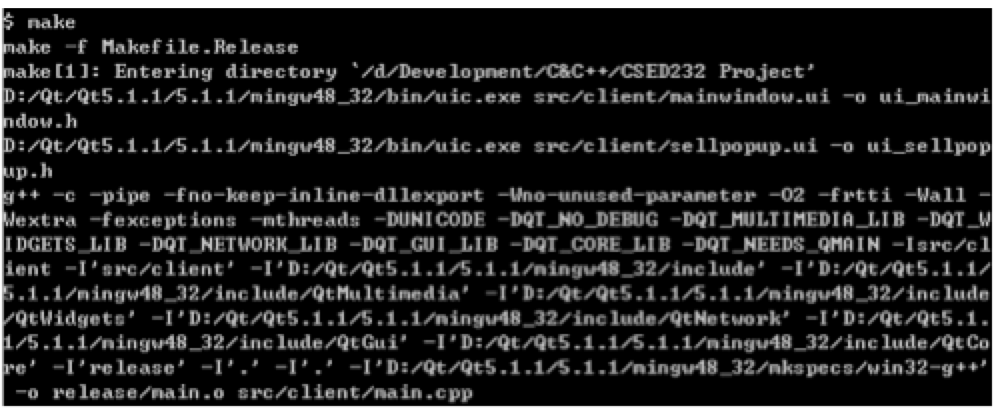
\includegraphics[scale=0.8]{images/compile2}
\caption{컴파일 과정}
\end{figure}

\section{Bluescreen 팀 구성}

\subsection{팀원 담당 업무 및 작성한 코드}

여러명이서 작업하기 위해 Git 소스버전관리 시스템을 활용하였고 github에서 hosting을 하였다. 소스코드를 여러명이서 함께 상호보완적으로 작업했기 때문에 오로지 혼자서 작성한 소스코드는 없고 팀원들이 한줄씩 추가하거나 삭제하면서 완성해나아갔다. 다음은 Github로 뽑은 소스코드 통계이다.

\begin{figure}[H]
\centering
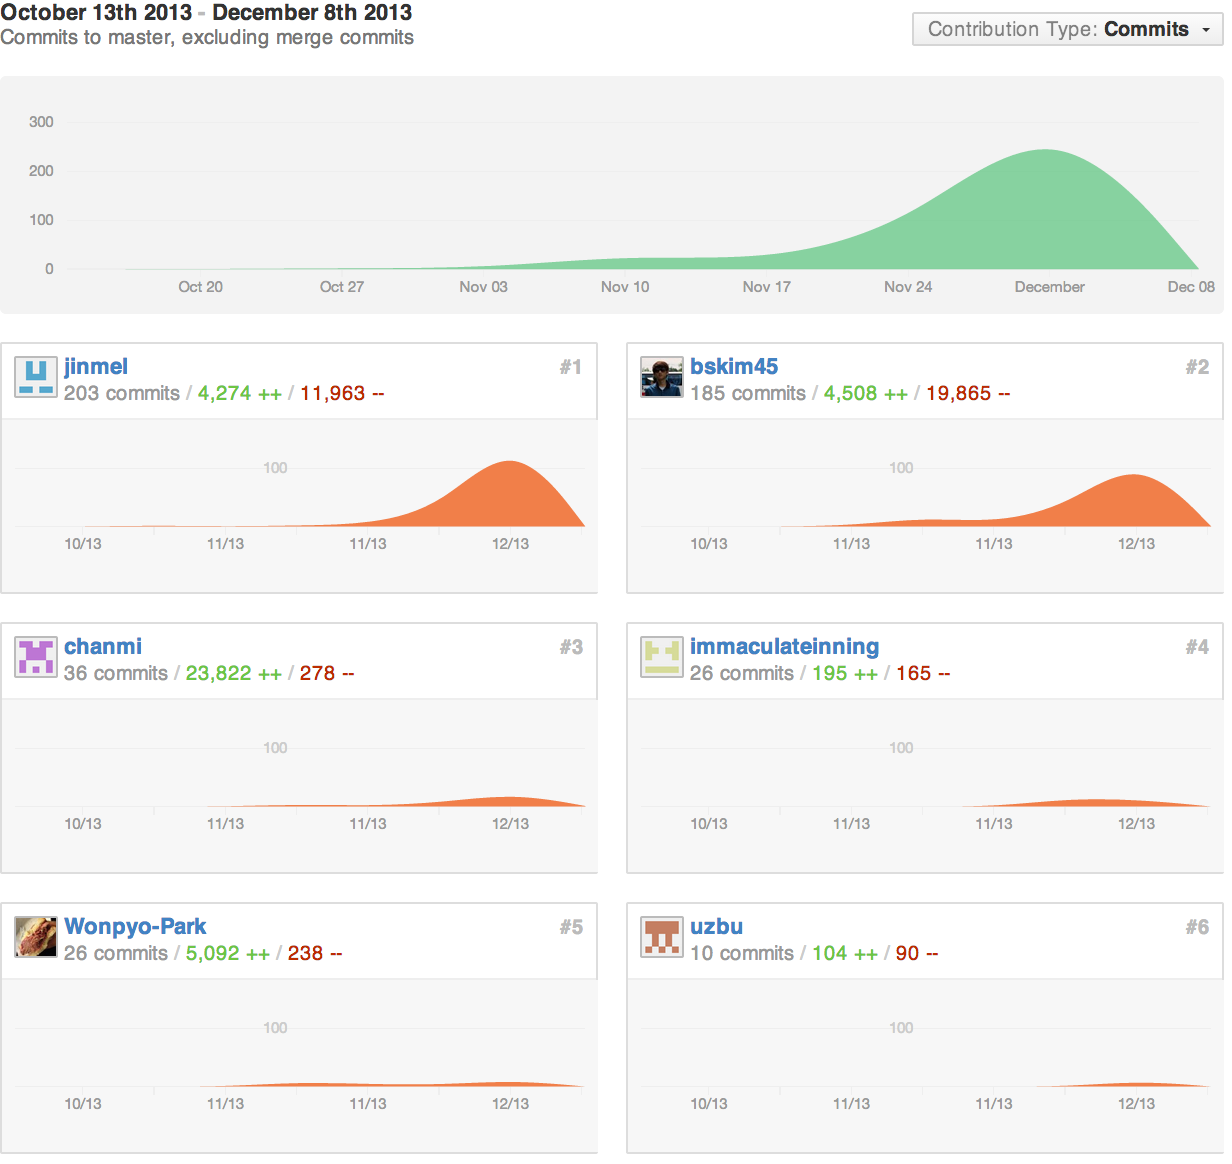
\includegraphics[scale=0.8]{images/github}
\caption{Github contributions}
\end{figure}

김홍기 팀원의 github오류로 인해서 통계에 나오지 않는데 79커밋이 존재한다. 

\begin{figure}[H]
\centering
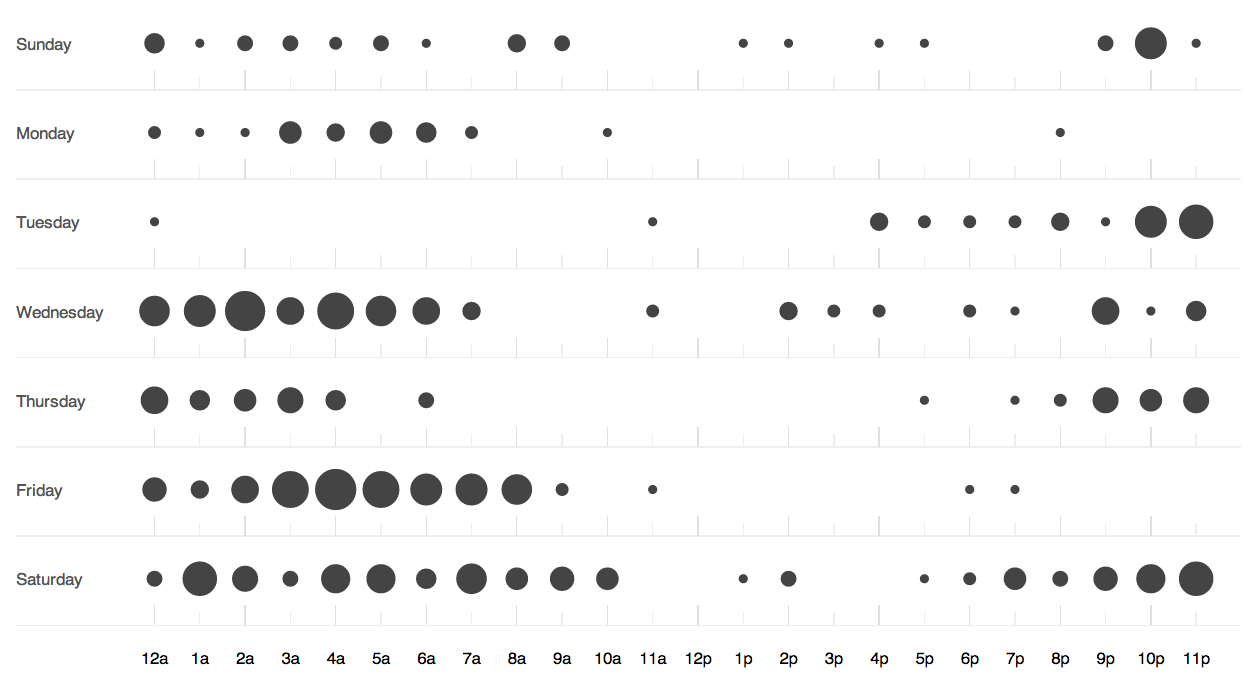
\includegraphics[scale=0.8]{images/github2}
\caption{Github activity punchcard}
\end{figure}

오후 10시에 모여서 밤을 샜기 때문에 커밋이 대부분 오후10시~오전6시에 몰려있다.

\subsection{팀원 평가}

\subsubsection{유찬미}
박진석 - 우리 팀의 개발 대장이다. 프로그래밍을 아주 잘하며 아는 것도 많다. 그런데 진석이가 프로그래밍을 잘하고 아는 것도 많은 이유는 다른 데 있는 것이 아니었다. 한번 프로그래밍에 빠져들면 집중력 있게 해낸다. 반복되는 코드를 작성해야 하거나 귀찮은 부분을 작성해야 할 때에도 투다다닥 키보드를 치면서 뚝딱뚝딱 해낸다. 그 엄청난 집중력은 정말 배우고 싶은 부분이다.
처음에는 성격이 무뚝뚝하고 차가울 줄 알았는데 놀자고 할 때 잘 놀고 업무를 해야 할 때에는 딱딱 해내며 팀원들이 모르는 것이 있을 때 친절하게 잘 설명해준다. 팀의 동생들에게 자상한 형의 이미지로 느껴져서 나도 모르게 '진석이 형' 이라고 부르게 될 정도였다. 

박원표 - 팀 내 분위기메이커였다. 평소에 애교가 많고 말이 많은 편이라 원표를 통해서 우리 조가 밝은 분위기를 항상 유지할 수 있었다. 말이 많다는 것은 어찌 보면 단점으로 작용할 수 있는 특징인데 우리 조에서는 원표가 이런저런 수다를 떨어서 팀원들끼리 서로 대화의 장이 열렸고 조원들이 처음 모였을 때 어색했던 분위기가 빠르게 완화될 수 있어 오히려 아주 좋은 점으로 작용하였다. 원표는 덜렁대고 허당인 면이 있으나 주변에서 놀려도 시무룩해하지 않고 더 재미있는 반응을 하여 자신을 희생하면서 좋은 분위기를 만들었다.
업무를 수행할 때에는 잡일이더라도 자신에게 주어진 일이라면 성실하게 열심히 해냈다. 목소리를 녹음하는 일을 원표에게 시켰을 때, 자신의 목소리가 들어가는 것이 민망하여 주저할까 싶었으나 전혀 개의치 않고 팀의 프로젝트를 위해 묵묵히 조용한 곳으로 가서 열심히 녹음하는 모습이 인상 깊었다. 원표가 열심히 만들어 온 리소스들은 예쁘지 않다는 이유로 쓰이지 않게 되거나 목소리 리소스가 좋지 않다는 평을 많이 받아서 많이 아쉽지만 우리 조원 모두 그가 얼마나 열심히 했는지는 알고 있을 것이다.

김홍기 - 리소스를 제작하는데 아주 탁월한 능력을 가지고 있다. 프로그램에 들어간 많은 리소스들이 홍기의 손을 거쳐서 탄생했는데 아기자기하고 귀여운 그림들을 잘 만들어내었다. 홍기도 원표처럼 팀의 분위기를 살리는 분위기메이커이지만 홍기가 한참 동안 조용히 있으면 잠시 후에 엄청난 리소스가 완성되어 있다. 리소스를 만드는 데 센스가 있고 노가다적인 작업이 많음에도 꿋꿋이 해내는 근성이 있다. 프로젝트 초반에 게임 설계 업무를 함께 하였는데 어떻게 하면 게임을 재밌게 할 수 있을지 잘 알고 있고 고민을 많이 한다. 전체적인 게임 룰을 짜는 데에 큰 역할을 하였다. 리소스도 잘 만드는데다가 내부 코드 구현도 열심히 참여하였다. 
성격이 착하고 엉뚱하고 재미있는 말을 많이 하여 밤샘 작업에 활력소를 불어 넣어 주었다. 


김범수 - 프로그래밍이면 프로그래밍 리소스면 리소스 못하는 게 없는 능력자이다. 처음에 범수가 UI를 담당하여 개발을 해 본 경험이 있다고 하여 UI를 중심적으로 업무를 분담했는데 UI도 잘 짜고 리소스 하나하나도 세련되고 예쁘게 잘 만드는데다가 프로그래밍도 빈틈없이 착착 잘 해냈다. 프로그래밍과 조 업무에 관한 아이디어를 많이 제시하였는데 효율적이고 좋은 아이디어들을 많이 생각해내어 프로젝트를 더 원활하게 돌아가도록 하였다. 
업무를 할 때에 아주 집중력이 참 좋고 근성이 있다. 프로그래밍을 하다가도 잘 되지 않는 부분이 있으면 끝까지 해결하였고 여러 팀원들이 함께 소스를 작성하는 과정에서 생긴 코드 conflict를 해결하는 데 쉽지 않은 작업이었어도 모두 resolve해내었다. 집중력이 좋다 보니 업무를 하는 데에도 효율이 아주 좋은데 그래서 남들이 소스코드 한 파일을 작성할 때에 범수는 소스코드 한 파일과 리소스 2개를 만들어내었다. 프로그래밍과 리소스 제작 그리고 여러 톡톡 튀는 아이디어와 센스로 이번 프로젝트에서 아주 큰 기여를 하였다.

이주현 - 처음 만났을 때에는 원표와 반대로 아주 말이 없는 캐릭터였다. 모두가 의견을 얘기하는 시점에도 조용히 사람들의 의견을 듣고만 있었고 본인의 의견을 말하는 경우는 내가 의견을 물어볼 때에만 겨우 얘기할 뿐이었다. 하지만 프로젝트가 점점 진행되면서 팀원들에게 친밀감을 느꼈는지 자신의 의견을 열심히 표현하였다. 
개발 경험이 없고 수학과라서 프로그래밍 보다는 상학 선배와 함께 math model을 설계하는 데 중점적으로 업무를 맡았는데 수치를 일일히 정하는 것이 쉽지 않았을 텐데도 적절한 model을 설계하여 게임을 원활하게 돌아가도록 하였다.

이상학 - 팀 내 최고학번으로 묵묵히 정신적인 지주 역할을 해주셨다. 학번이 높은 만큼 연륜이 있었고 밤샘 작업으로 인해 굶주린 조원들에게 야식을 사주면서 좋은 선배 역할을 해주셨다. 
개발 경험이 없어서 프로그래밍에 큰 기여는 못할 것 같다고 하였지만 맡은 일에 대해서는 정말 열심히 하였고 부지런한 성격이었다. 조 모임 시간에도 일찍 와서 조 모임을 준비하고 있었고 프로젝트 마감일이 다가오면서 조원들 전체적으로 밤샘 작업으로 인해 피곤해하였는데도 말없이 부지런히 조모임에 오셔서 업무에 집중하였다. 상학 선배의 그런 모습이 매우 듬직했고 드러내진 않았지만 모두의 마음속에 정신적인 지주가 되었을 것이다.

\subsubsection{박원표}
유찬미: 팀의 조장. 
처음 프로젝트 조 편성이 되고 일주일이 채 되기 전에 조원들에게 모두 연락하고, 빠른 일처리 진행으로, 어떤 조보다도 빠른 프로젝트 진행이 가능하게 만든 장본인이다. 나는 이번 객체 프로젝트를 진행하면서, 찬미누나의 리더쉽을 통해서 많은 것을 배울 수 있었다. 찬미누나는 넉살 좋고 착하게 생긴 이미지로 팀의 분위기를 화기애애 하게 했지만, 동시에 지각 체크나 각자의 업무분담에 대해서는 확실한 선을 그어 팀의 프로젝트 진행에 큰 도움이 되었다. 또한 찬미 누나는 이런 팀으로 이루어진 개발 프로젝트가 처음임에도 불구하고 주변의 경험이 많은 팀원들에게서 의견을 수합해서 모두가 동의할 만한 올바른 방향으로 프로젝트를 진행해 나갔다. 또한 개발과정에 있어서도 열심히 참여 하고 배우면서, 자신이 팀에 기여할 수 있는 최대의 방향으로 개발에 기여했다.
찬미누나는 순박하게 생긴 외모 속에서 묻어나는 카리스마를 통해서 나는 팀을 이끄는 새로운 방식을 배운 것 같다. 화기애애한 가족 같은 분위기로 조를 이끌어 나가고 동시에, 할일 은 확실히 하는 누나의 리더쉽은 후배로써 옆에서 많이 배울 수 있었다.

박진석: 팀의 개발 디렉터.
 진석이형은 수 많은 개발 경험으로 막막 하였던, 게임 개발을 끝까지 밀고 나갈 수 있게 한 장본인이다. 진석이 형은 다른 팀원들이 게임 개발에 참여하기 전, 팀원들이 편하게 작업을 할 수 있도록 Framework를 개발 하여 다른 팀원들이 편하게 개발에 참여할 수 있도록 하였다. 같이 조 프로젝트를 해보니, 처음에 ‘시크’하고 ‘센치’ 하였던 첫 인상과는 달리 상당히 유머감각 있고훈훈한 은근 동네 형 같은 포근함을 느낄 수 있었던 은근히 정가는 멋진 형이었다. 
	내가 진석이 형을 보면서 가장 놀란 점은 ‘근성’ 이였다. 처음 사용하는 Qt였지만 자신이 완벽하게 이해하고 완벽히 사용할 수 있도록 Qt를 파고 들었고, 프로젝트를 진행하는 동안 만들어진 프로젝트 결과에 만족하기 보다는 여기서 어떻게 하면 더 낳아 질 수 있을까? 라고 의문을 던지고 또 결국에는 해내는 모습을 보여줬다. 그리고 그런 모습을 통해서 나의 근성이 아직은 부족하다는 사실을 깨닫게 되었고, 큰 귀감이 되었다. 그리고 뛰어난 개발자이며 경험이 많아 개발에 관련한 많은 부가적인 지식을 얻을 수 있었다.

김홍기: 게임 기획자, 팀의 리소스 메이커 및 개발자
	홍기는 만족을 모르는 최고의 기획자, 리소스메이커이다. 홍기는 게임 개발 내내 보다 더 낳은 리소스를 만들 수는 없을까? 그래픽을 더 낳게 할 수는 없을까? 게임 진행을 이렇게 바꿔보면 어떨까? 의문을 던져가며 더 나은 게임을 완성할 수 있도록 기여 하였다. 처음에는 보드 리소스를 내가 간단히 프로토 타입형식으로 제작하여 게임에 사용하였는데, 홍기는 이를 몇 시간 동안 고민하더니 확실히 더 나은 디자인으로 완성하였다. 게임 리소스 작업은 공대생한테 맞지 않고, 오래 동안 고민하고 수정해야만 하는 고된 작업임에도 홍기는 리소스 작업에 매진하여 ‘포스텍 마블’의 뛰어난 그래픽이 완성 될 수 있었다.
	홍기는 게임의 기획하는 단계에서도 빛이 낳는데, 꿈이 프로그램 개발자이고 게임에 관심이 많은 만큼, 눈이 반짝거리면서 기획에 참가하여 좋은 아이디어로 구체적인 안을 제시 하였다. 우리 포스텍 마블의 진행 방식은 홍기로부터 비롯되었다고 하여도 틀린 말은 아닐 것이다. 
	이런 홍기는 게임 개발 과정에서 ‘열정’을 보이며 프로젝트를 훌륭하게 이끌어 나갔다. 나는 이런 홍기의 열정을 통해 많은 것을 배울 수 있었으며, 앞으로 미래가 기대되는 친구이다.


김범수: 코드 결벽증을 가진 완벽주의 개발자. 싱글톤 인스턴스의 변태, 게임 개발왕
	진석이 형과 함께 우리 프로젝트 최고의 개발자는 바로 범수이다. 범수는 많은 게임 개발 경험으로써 팀에 큰 기여를 하였다고 할 수 있다. 범수는 처음 버전 관리 프로그램인 git을 써서 혼선을 빚는 팀원들에게 친절하게 git 사용법을 알려주고, conflict가 일어나도 당황하지 않고 code resolve에 앞장 섰다. 나같이 처음 개발을 진행하고 협업을 한 사람 입장에서 범수는 멘토로써 나에게 나침반 같은 역할을 했다. 범수는 다른 팀원들이 개발을 진행하고 있지 않는 시간에도 틈틈히 많은 시간을 투자 하여 프로그램 개발을 수행 하였고, 덕분에 제시간 안에 게임을 개발할 수 있었다. 특히, 범수가 짠 코드를 보면서 나는 잘 짜여진 코드가 어떤 것이 구나에 대해서 배울 수 있었다. 한 예시로 범수는 싱글콘 인스턴스 기법을 활용해서 dice 객체를 구현했는데, 이를 통해 실제 개발 기법 등을 배울 수 있었다.
	범수는 개발경험이 다분한 학생으로써 팀을 위해서 조별 모임 중이 아닌 시간에도 최선을 다해 프로젝트에 기여하였고, 다분한 노력으로 버그들을 해결하고 올바르게 작동 될 수 있도록 개발에 최선을 다하였다. 또한 특유의 위트있는 성격으로 팀의 분위기를 한층 돋구었다고 할 수 있다.


이주현: 수학과의 Math Model 왕 
	주현이는 맡은 바를 성실히 다하는 Math model의 왕이 아닐까 싶다. 수학과 특유의 센스로 수학에 대한 능력이 뛰어나 훌륭한 게임 math model을 만들 수 있었지만, 이 역시도 직접 한번 게임을 손으로 시뮬레이션 해가면서 진행해 봐야지만 정확히 알 수 있었다. 그리고 주현이는 이러한 과정을 직접 ‘노가다’를 해가며 체크를 반복하였다. 그의 노력 덕분에 우리는 보다 정교한 Math model로 정말 오르락 내리락 하며 게임의 승패가 전략에 의해 정해지는 치열한 게임을 만들 수 있었다. 
	이외에도 주현이는 기타 많은 개발, 리소스제작 업무를 보조해주며 도움을 많이 주었다. 그러나 이러한 과정에서 주현이는 큰 불만 없이 자신의 일을 묵묵히 수행 하였고, 팀의 도움이 많이 되었다. 나는 주현이 같이 뛰어나고 성실한 친구가 함께 프로젝트를 하게 되어서 참으로 고마운 일이라고 생각한다.

이상학: Math Model 디자이너, 정신적 지주
	상학 선배는 팀의 최고 연장자인 만큼 무게 중심이 있이 팀을 이끌어 갔다. 확실 연장자이신 만큼 남들보다 신뢰감이 있고 무게감이 있으셧다. 그리고 상학이형을 보고 있다보면 진심으로 신뢰감이 생길 수 밖에 없었다. 상학이 형은 주현이와 함께 Math Model을 디자인 하셨는데, 주현이와 함께 손 시뮬레이션을 돌려가시면서, 보다 정확한 모델을 만들기 위해서 노력하셨다. 내가 상학이 형을 보며 신뢰감이 들었던 이유는 상학이 형은 자신의 담당 업무인 Math Model이 완료가 된 후에, 아무도 신경 쓰지 않았던, 보고서 같은 부분을 직접 찾아서 묵묵히 진행 하셨다. 그 외에도 주석 같이 힘들고 고된 작업을 묵묵히 훌륭하게 수행하셨다. 
	팀에서 신경 쓰지 못했던 부분을 세밀하게 점검하시고, 직접 찾아서 성실히 수행 하시는 모습을 통해서 나는 ‘신뢰감’을 주는 사람이 어떤 사람인가에 대해서 느낄 수 있었고 이를 통해 많이 배울 수 있었다. 

\subsubsection{이상학}

유찬미: 유일한 여성 조장. 그 하나만으로도 빛나는 존재가 아닐까 싶다. 이번 OOP를 수강하는 학생 중 가장, 조장에 어울리는 사람이라고 자신할 수 있다. 많은 조장들이 업무 수행 능력(의지)과 리더십 둘 중 하나만 가지고 있는 데에 비해, 유찬미 조장은 2개 모두를 가진 완벽한 조장이라 할 수 있다. 업무 수행 능력으로 보자면, 원래 조장이 맡은 main 관리, 보고서 작성, 발표 준비를 넘어 내부 코딩과 그 설계까지 핵심적으로 참여하는 열정적인 모습을 보이고, 또한 그 성과를 보였다. 
업무 수행 능력도 좋았지만, 유찬미 조장이 더욱 빛났던 곳은 리더쉽 부문이었다. 7명으로 이루어진 사상 초유, 최대의 프로젝트에서 한 명 버려지는 사람 없이, 모두가 맡은 일을 빠진 것 없이 해냈다는 점은, 정말이지 조장의 리더쉽을 칭찬할 수 밖에 없다. 역할 분배, 조원 소집, 의견 수렴, 조원 독려 및 사기 진작, 과제 외 활동까지 빠진 점을 찾기가 힘들다. 단언컨대 유찬미 조장은 가장 완벽한 조장입니다.

박진석: 코딩의 쌍두마차 중 일인. 박진석 조원이 없었다면 이 프로젝트는 존재할 수 없었을 거라고 단언할 수 있다.  7명의 코드를 합친다는 것은, 소프트웨어 디자인을 배우지 않은 우리로서는 사실상 불가능에 가까운, 매우 힘든 일이다. 하지만 그가 제안한 ‘github’, 그것은 우리들의 프로젝트에 날개를 달아주었다. 초기에는 그런 유틸리티까지 필요한 것인가 의아했지만, 시간이 가면 갈수록 그 위대함을 느낄 수 있었다. 또한 개발을 하면 할수록 느껴지는 박진석 조원의 끝을 모르는 디버깅 실력과, 누구나 쉽게 알아볼 수 있고, 이용할 수 있는 코드를 짜는 능력은, 프로젝트 기간 내내 나에게 깊은 인상을 남겼다. 
박진석 조원의 가장 큰 장점은, 포기를 모르는 정신과 현실에 안주하지 않고 계속 발전해 나가려는 진취적 의지라고 본다. 코딩 내내 많은 어려움에 부딪히고, ‘여기까지만 하자’하고 끝낼 수도 있었던 많은 부분에서, 그의 의지는 그런 패배자 근성을 결코 용서치 않았다. 나이는 나보다 어리지만 배울 게 참 많았던, 조 내의 든든한 Mentor였던 박진석 조원, 같이 일하고 싶은 최고의 파트너라고 할 수 있다. 

김범수: 박진석 조원과 함께 팀 내 주역 코딩을 도맡은 김범수 조원. 박진석 조원이 프로그램의 뼈대를 만들었다면, 김범수 조원은 그 뼈대를 움직이기 위한 심장을 만들었다고 할 수 있다. 김범수 조원은 Qt의 지배자라고 할 수 있다. 모두에게 생소했던 개발환경 Qt. 김범수 조원은 우리에게 필요한 Qt의 특성과 기능을 누구보다 빠르고 자세하게 조원들에게 전달하여 프로그램 개발에 필요한 (인적) 환경 구축에 큰 기여를 했다. 또한 ‘이것을 어떻게 구현할까’, 한 때는 빼버릴까도 생각했던 기능들, 김범수 조원은 끝내 모두 Qt로 구현하는 데에 성공하였다.
김범수 조원의 가장 인상 깊었던 점은, 그의 지칠 줄 모르는 체력과, 한번 앉으면 일어날 줄을 모르는 뚝심이었다. 한번 코딩을 시작하면 멈추지 않는 김범수 조원의 끈기와 인내심에는 혀를 내두를 수밖에 없었다. 어떤 어려운 조건도 결국에는 구현해 내는 그의 능력과 끈기. 프로젝트 내내 참 배울 점이 많았던 친구였다.

김홍기: 우리의 프로그램을 아름답게, 그럴듯하게 만들어낸 1등 공신인 김홍기 조원. 김홍기 조원은 말 그대로 ‘리소스’의 창조주였다. 단순히 그림판에 그려진 아이들 낙서처럼 될 수도 있었던 우리의 ‘포스텍 마블’을 정말로 게임으로 만들어준 장본인이라고 할 수 있다. ‘허접함’을 용납치 않는 리소스를 향한 그의 장인 정신은 ‘포스텍 마블’의 격을 몇 단계는 끌어올렸다고 본다.
무엇보다 마음에 들었던 김홍기 조원의 장점은 흔들리지 않는, 그러면서도 유한 그의 성품이었다. 모두가 흔히 말하는 ‘멘탈이 붕괴된’ 상황에서도 그는, 변하지 않는, 평소의 부드러운 김홍기의 모습을 언제나 고수했다. 마치 득도한 고승과도 같던 그의 모습을 보면서, 나는 자신의 
약한 멘탈을 부끄러이 여기며 자신을 다독일 수 있었고, 원래의 상태로 회복할 수 있었다.

박원표: 누구도 부정할 수 없는 팀 ‘블루스크린’의 분위기 메이커 박원표 조원. 그의 존재가 없었다면, ‘블루스크린’은 장담컨대 배는 어두운 암울한 조가 되었을 것이다. 그는 자신이 망가지는 것을 두려워하지 않고, 조원 간의 원만한 융화를 이끈 팀의 정신적 지주라고 할 수 있었다. 유찬미 조장이 직접적으로 우리를 이끄는 존재였다면, 박원표 조원은 우리를 보이지 않는 곳에서 알게 모르게 묶어준 ‘다크나이트’ 라고 칭할 수 있을 것이다. 그의 쾌활하고 순수한 성격은 모든 조원의 마음을 힐링해주는 청량수와 같은 존재였다. 긴 밤샘 작업을 무사히 끝마칠 수 있게 한 그의 능력과 노고에 큰 찬사를 보낸다.
또한 그는 톡톡 튀는 아이디어의 보고였다 각종 참신한 아이디어들이 그의 머리 속에 자리잡고 있었다. 가히 창의IT과의 학생이라 할 수 있는 모습이었다.

이주현: Math Model과 Algorithm의 화신 이주현 조원. 이주현 조원의 data와 함수에 관한 정확한 분석은 우리의 ‘삽질’을 상당히 줄여주었다. 아마 그의 존재가 없었다면, 보고서를 쓰는 지금도 계속 버그와 언밸런스의 홍수 속에 쓸려가고 있지 않았을까 하는 생각이 든다. 그의 Math Model 로 게임 내 수치 조정 시간을 상당히 줄여주었고 또한 게임의 밸런스를 알맞게 맞추는 그의 능력으로 ‘포스텍 마블’이 정말 게임이 되었다고 생각한다.  
이주현 조원은 언제나 묵묵히 자신의 맡은 일을 해내는 믿을 수 있는 조원이었다. 어떤 일을 받아도 불평 없이, 자신의 일을 완벽하게 해내었다. 만약 믿을 수 있는 파트너를 원한다면. 이주현 조원을 동료로 삼는 것이 ‘베스트 초이스’가 아닐까 생각한다.


\subsubsection{이주현}

유찬미 – 조장. 처음으로 조원을 모았다는 점에서 조장이 되었는데, 조장에 걸맞는 능력을 프로젝트 기간 동안 보여주었다고 생각한다. 리더십이 필요한 분야에서 능력을 발휘하였으며, 개발 이외의 부분에서는 다른 조원 전체를 휘어 잡을 정도의 리더십을 보여주었다. 다른 팀 프로젝트와는 달리 이번에 팀 프로젝트를 가면서 잦은 회식과 밤샘이 있었는데, 조장이 다른 사람이었더라면 잦은 밤샘과 회식은 어려웠을 것이다. 개발에서도 개발 경력은 없었지만 자신이 맡은 일을 열심히 하는 모습을 볼 수 있었다.

박진석 – 프로그래밍에 있어서 사실상의 리더 역할을 했다고 할 수 있으며, 프로젝트의 전체적인 방향을 제시한 역할을 하였다. 컴퓨터공학과가 아님에도 불구하고 뛰어난 코딩 실력을 가지고 있었고, 코딩 디렉터 역할 뿐만 아니라 실제 코딩에 있어서도 가장 활발한 활동을 보였다. 체계적인 프로젝트 진행을 위하여 많은 조언을 해 주었고, 프로그래밍에 대한 해박한 지식을 유감없이 발휘해 주셨다.

박원표 – 전반적인 코딩과 리소스를 담당했으며, 팀 내의 분위기 메이커 역할도 하였다. 이번 프로젝트 규모가 컸던 만큼 밤을 새는 일이 잦았는데, 밤샘이 계속되면서 잘 되지 않으면 짜증이나 불만이 나올 수 있는데 그럴 때 마다 팀의 활력소 역할을 하였다. 프로그램의 마지막 부분을 만드는 데 어려움이 있었지만, 충분한 능력을 발휘해서 마지막 장면을 완성해 주었다.

김범수 – 프로그램의 전반적인 개발을 담당하였으며, 개발 경험을 잘 살려 많은 양의 소스코드를 처리하고, 기획 단계에서부터 다른 팀과는 달리 git를 사용하자고 제안하여 효율적인 과정으로 협업을 할 수 있게 만들었다. git를 사용하면서 사소한 충돌, 오류가 발생하는 경우가 있었는데, 그 때마다 문제를 해결하는 모습도 보여주었다.

김홍기 – 전반적인 프로그램 코딩과 리소스를 담당하였으며, 특히 리소스가 인상 깊었다. 양질의 리소스를 만들어 기대한 만큼 높은 퀄리티의 게임을 만들 수 있게 했다. 프로그램 개발에 있어서도 개발 경력이 있는 점을 이용하여 큰 어려움 없이 프로젝트가 완성되는데 큰 공헌을 했다. 기존의 리소스를 그대로 사용했다면 평범한 과제처럼 보일 수도 있었던 게임을 그래픽적으로 손색이 없는 게임으로 바꾸어 주었다고 말할 수 있겠다.

이상학 – 게임에 적용할 model을 같이 만드는 역할을 했는데, 많은 아이디어를 제공했다. 프로젝트 팀 내 최고학번이신데, 다른 조원들과 학번 차이가 있음에도 불구하고 열심히 참여하시려 하시고, 게임의 모델을 짜는 일 이외에도 할 수 있는 일은 다 하시려고 하는 모습을 보여주셨다. 코딩에는 관여를 많이 하시지 않았지만, 모델, 보고서 등의 일에서 큰 도움을 주셨다.

\subsubsection{김범수}
조장 유찬미:
찬미 누나가 팀장이었기에 우리 조가 존재했다고 할 수 있을 정도로 뛰어난 리더십으로 팀을 하나로 이끌어 주었다. 누나는 가장 먼저 주도적으로 팀원들을 모았으며, 첫날 서먹서먹한 분위기에서도 주제를 잡고 팀이 앞으로 나아가야 할 방향을 정할 수 있도록 해 주었다. 항상 친근한 자세와 웃음으로 팀원들이 융합될 수 있도록 해 주었을 뿐만 아니라, 팀원들이 지각했을 때와 같이 필요할 때는 날카로운 카리스마로 팀의 기강을 유지해 주었다. 비단 리더십뿐만 아니라, 개발에도 열정적으로 참여하여 프로그램 설계와 내부 구현에도 함께 참여하였다.

개발 헤드 박진석:
 진석이형의 풍부한 개발 경험은 우리 조의 핵심 자원이 되었다. 진석이형에게 단연 빛났던 점은 ‘끈기’와 ‘근성’이었다. 비록 풍부한 개발 경험이 바탕이 되어 주었으나, 처음 접해보는 Qt라는 프레임워크를 완전히 이해하려고 노력하였으며, Qt를 이용해 우리 게임을 구현하는 데 필요한 프레임워크를 제작하여 팀원들이 보다 쉽게 프로그램을 구현할 수 있도록 해 주었다. 특히, 현재 개발 상황에 만족하지 않고 끊임없이 개선사항을 연구하는 모습과, 형의 멈출 줄 모르는 디버깅 실력은 팀이 중간에 포기하지 않고 의도했던 모든 기능을 구현할 수 있도록 해 주었다. 형의 이런 모습을 보며 조금만 로직이 복잡하면 구현을 망설였던 나의 모습을 반성해 볼 수 있었다.

게임 디렉터 김홍기:
 홍기는 개발, 디자인 리소스, 개임 기획 모두에 정통한 만능 프로그래머이다. 개발 실력은 물론이거니와 수많은 미려한 리소스와 사운드로 프로그램의 완성도를 높여 주었다. 아무리 뛰어난 프로그램이라도 겉모습이 아름답지 않으면 사용자들은 외면하기 마련이다. 홍기는 자칫 식상해질 수 있었던 우리 게임에 아름다운 그래픽과 사운드를 더해 완벽한 게임으로 거듭날 수 있게 해 주었다. 뿐만 아니라, 어렸을 때부터 게임을 기획해 왔을 정도로 게임 기획에 능통하여 우리 게임을 디자인 하는 데 큰 도움이 되었다. 아마 포스텍 마블의 전체 기획은 홍기의 머리에서 나왔다고 해도 과언이 아닐 것이다. 이렇듯 홍기의 다재다능한 능력은 개발 과정에서 적재적소에 투입되어 개발이 원활하게 이루어질 수 있도록 해 주었다.

분위기 메이커 박원표:
 원표는 단연 우리팀의 분위기 메이커이다. 원표의 멈출 줄 모르는 입답은 팀원들을 항상 즐겁게 해 주었으며, 특히 밤샘 작업을 할 때에 팀원들의 활력소가 되어 주었다. 분위기 메이킹 뿐만 아니라 개발과 리소스 디자인에 대한 열정이 높아서, 핵심적인 개발 과정에 참가했을 뿐만 아니라 홍기를 도와 리소스를 만들어 게임의 완성도를 높이는 데 힘썼다. 특히, 원표는 게임 사운드 제작을 담당해, 게임을 할 때마다 우리는 원표의 목소리를 들을 수 있게 되었다. 창의IT융합공학과 답게 창의적인 방법으로 게임의 가장 핵심적인 요소인 ‘재미’와 ‘쫄깃함’을 부여한 것이다. 그는 ‘요란한 빈 수레’가 아닌 ‘무겁지만 빠르게 움직이는 수레’였다.

메스 모델러 이주현:
 주현이는 수학과답게 게임의 디자인을 담당해 주었다. 게임에 있어 레벨 디자인과 메스 모델링은 핵심적인 요소 중 하나로, 이것이 제대로 디자인 되지 않으면 아무리 잘 만든 게임이라도 재미가 없게 된다. 만약 주현이의 정확한 수학 모델링이 없었다면 우리는 게임을 이미 완성했음에도 불구하고 게임의 밸런스를 맞추기 위해 아직까지도 게임을 플레이해 보고 있었을 것이다 또한, 주현이의 맡은 일을 항상 묵묵하게 해내는 모습은 어떤 일을 할 때 불평불만이 많은 나의 모습을 되돌아볼 수 있게 해 주었다.

우리 팀의 영원한 멘토 이상학:
 우리 팀의 최고 학번답게 팀원들의 멘토가 되어 찬미 누나와 함께 팀을 이끌어 주셨다. 특히, 팀이 엉뚱한 방향으로 가거나 갈피를 잡지 못할 때 해주시는 형의 조언 한마디는 안개 낀 바다의 등대가 되어 팀을 올바른 방향으로 이끌어 주었다. 뿐만 아니라, 주현이를 도와 게임 기획과 디자인의 전반을 담당했을 뿐만 아니라, 레퍼런스 문서를 제작하여 팀원들이 개발하는 과정에서 별도의 혼란 없이 프로그램을 구현할 수 있도록 해 주셨다.

\subsubsection{김홍기}
유찬미: 우리 포스텍 마블의 팀장. 찬미 누나는 이번 프로젝트를 통해서 처음 만나게 되었다. 평소에 RA라는 것은 알고 있었지만 직접 알 기회가 전혀 없었다. 이 프로젝트가 종료되는 시점인 지금 생각해보면 누나가 왜 RA가 되었는지 이해할 수 있었다. 찬미누나의 리더십은 이 프로젝트에서도 고스란히 드러났다. 다른 조보다 훨씬 빨리 조원들과 연락하여 모임을 잡았다. 그 결과, 다른 팀에 비해서 조금 더 여유를 가지고 일찍 프로젝트를 시작할 수 있었다. 평소에는 잘 웃으시고 팀의 분위기를 이끌면서도 확실하게 해야 될 때에는 진지하게 프로젝트 진행에 임하셨다. 실제로 개발하는 것이 이번이 처음이지만 배우려고 노력하시는 모습을 많이 보여주셨다. 게다가 거의 프로젝트 모든 분야에서 적극적으로 참여하시는 모습을 보여주시면서 우리 팀의 참여를 유도하셨다. 찬미누나는 말 그대로 팀을 성공으로 이끄는 모범적인 리더였다. 이번 프로젝트에서 찬미누나를 보면서 진정한 리더란 무엇인지에 대해서 많은 답을 얻게 되었다.

박진석: 이번 프로젝트의 메인 개발자라고 할 수 있다. 진석이형은 비록 게임 개발은 처음이셨지만 예전부터 다른 분야의 개발을 잘 하셨기 때문에 프로젝트의 많은 코드를 작성하셨다. 게임 개발에 적합하지 않은 QT에서 Framework를 작성하셔서 개발이 훨씬 효율적으로 진행될 수 있었다. 다들 QT를 처음 써보지만 진석이형은 QT를 짧은 시간만에 익히셔서 팀원들이 QT에서 막히는 부분이 있다면 많이 해결해주셨다. 진석이형은 처음 봤을 때는 조용한 사람인 줄 알았지만 같이 모여서 프로젝트를 진행할수록 그렇지 않다고 생각했다. 조원과 의사소통 하며 각자가 어디 부분의 코드를 작성해야 하는지 조정하였고 프로젝트의 전체적인 구조를 만드셨다. 개인적으로는 진석이형을 보면서 정말 뛰어난 개발자라고 생각했다. 프로젝트에 대한 열정, 그리고 오랫동안 집중하여 코딩하는 모습은 꼭 본받고 싶은 점이었다. 이번 프로젝트에서 진석이형을 통해 멋진 개발자가 되기 위해서 열심히 노력해야겠다고 생각했다.

김범수: 믿을 수 있는 동료. 범수와는 같은 과 동기이며 해카톤 대회에서 같은 팀으로 참가한 경험이 있다. 처음에 범수와 같은 팀이 되어서 정말 재미있는 프로젝트를 할 수 있을 것이라 생각하였고 실제로도 그랬다. 범수는 이번에도 git을 사용하자고 제시하였는데 정말 좋은 선택이었던 것 같다. 7명이란 대규모 인원에서 공동작업을 한다는 것은 각자의 소스코드를 합치는 것만 해도 굉장히 힘든 일이다. 하지만 범수의 제안으로 인해 git을 사용하여 이러한 작업을 훨씬 수월하게 할 수 있었다. git을 조원들에게 가르치거나 문제가 발생했을 때 해결하는 것은 범수가 거의 다 하였다. 또한 범수는 게임 개발의 경험이 많았기 때문에 게임을 위한 코드 작성의 방법론을 제시하였다. 범수의 방법론을 바탕으로 우리는 보다 효율적이고 객체 지향적인 코드를 작성할 수 있었다. 저번에 범수와 같은 팀이었을 때는 하루 동안만 같이 일했지만 이번 프로젝트를 통해서 장기간 같이 일하게 되었는데 역시나 배울 점이 많았다. 범수의 끈기와 깔끔한 코드를 보면서 감탄한 적이 정말 많았다. 그리고 범수와는 죽이 잘 맞아서 같이 일을 하면 정말 즐거워서 같이 일기 즐거운 동료이다.

박원표: 원표는 같은 분반 동기로써 같은 팀이 되어 되게 반가웠다. 원표는 창의적인 아이디어가 넘쳐나고 끈기와 열정이 있는 친구라는 것을 알고 있었기 때문이다. 그리고 주변 사람들을 즐겁게 해주는 보이지 않는 힘이 있었다. 원표의 이러한 능력은 이번 프로젝트에서도 발휘되었다. 내가 생각하지 못했던 요소들을 더하여 게임을 좀 더 재미있게 만들었다. 또한 여러 방면에서 재능을 보였던 원표는 코드, 리소스, 사운드에 대해 일을 배정받으면 묵묵히 처리하는 것이 멋졌다. 게다가 그는 우리 팀에서 활기를 부여하는데 큰 공헌을 하였다. 자칫하면 딱딱한 팀 프로젝트가 될 수 있었지만 원표의 존재로 인해 다들 웃으면서 일을 할 수 있었다. 팀에 즐거움을 제공하면서 일 처리 능력이 뛰어난 원표는 한마디로 만능이었다. 원표를 통해서 팀 프로젝트의 분위기가 얼마나 중요한 지 알 수 있었다.

이주현: 주현이는 수학과 친구로써 상학선배와 math model을 담당하였다. Math modeling에서 주현이는 수학과의 능력을 유감없이 발휘하였다. 처음 코드를 작성할 때 수치는 모두 더미로 작성했었다. 게임이 어느 정도 완성된 이후 math model을 적용시킨 결과 게임의 밸런스가 잘 맞아떨어졌다. 너무 지루하지도 않고 너무 빠르지도 않았다. 손으로 시뮬레이션 하면서 수치를 계속 수정하며 반복하는 일이 결코 쉬운 일이 아닌데 불평하지 않고 묵묵히 모델링을 하였다. 아무리 화려한 게임이라도 밸런스가 안 맞으면 우수한 게임이라고 생각하지 않기 때문에 주현이의 math modeling은 게임의 핵심이라고 할 수 있다. 또한 보고서에서도 각 코드의 분석과 주석을 다는 작업을 성실하게 해주었다. 이번 프로젝트에서 주현이를 보면서 성실한 능력이 얼마나 부럽고 멋진 것인지 깨달을 수 있었다.

이상학: 상학선배는 프로젝트에서 가장 높은 학번이셨다. 팀원들의 잦은 밤샘작업으로 힘들어할 때 많이 다잡아주셨다. 그리고 주현이와 함께 손 시뮬레이션을 하면서 math model을 작성하여 게임의 완성도를 높여주셨다. 세세한 부분에서 밸런스를 맞추기 위해서 이벤트 블록에서의 이벤트도 조정하셨다. 또한 코드를 작성하다가 문법에서 막히는 부분이 있다면 조언을 해주셔서 문제를 쉽게 해결할 수 있었다. 게다가 보고서의 작성을 주도하셔서 이끄셨다. 여러 사람들의 의견을 조율하여 보고서를 작성하고 통합하는데 큰 공헌을 하셨다. 이번 프로젝트를 진행하며 상학선배를 보면서 많은 것을 깨달았다. 높은 학번으로써 여러 부분에서 조언을 해주시며 팀원들에게 신뢰를 주었던 것을 보면서 나도 나중에 저렇게 되고 싶다고 생각했다.


\subsubsection{박진석}

유찬미: 조장으로서의 역할을 충실히 하였다. 덕분에 조원들이 성실히 모임에 나왔고 좋은 분위기에서 열심히 할 수 있었던것 같다. 먹으러 다니는것을 좋아하여 내가 외식하는걸 좋아하는데 항상 기대하고 나오게 되었다. 조개구이도 처음먹어보고 아무튼 조장이 주도적으로 행사를 기획하여 즐거웠다. git을 처음쓰면서 많이 헤메면서도 짜증내지 않고 꾸준히 노력해줘서 고마웠다. 

김범수: 처음에 3조에 들어왔을 때 git을 쓰지 않으면 누군가는 7인분의 일을 할 것이고, 그리고 그게 내가 될것 같아서 일부러 개발을 못하는척하고 나서지 않으려고 했는데 범수가 앞장서서 git을 쓰자고 해서 이 조는 희망이 있다고 생각하게 되었다. 포애퍼의 에이스로 리소스 제작부터 개발까지 나를 많이 도와주어서 고마웠다. 나는 리소스 편집이나 제작을 꺼려하는편이고 리소스마저 코드로 구현하려고 하는데 범수는 포토샵이랑 파워포인트를 쓰면서 리소스에서 장인정신을 발휘하는것을 보고 내가 부족한면을 깨닫게 되었다. 

김홍기: 포애퍼의 회장으로서의 포스를 잘 보여준것 같다. 리소스를 공장처럼 찍어내었고 개발도 많이 도와주었다. 내가 요구하는 리소스라던가 사소한 부분을 귀찮아하지 않고 모두 척척 해내어서 고마웠다. 

이주현: 수학과로서 매스모델을 잘 만들어주었다. 게임의 QA를 하였고 버그를 많이 찾아내었다. 매스모델을 잘 설정하여 게임의 밸런스를 잘 조정하였다. 게임 특성상 루틴이 복잡하여 버그가 많이 발생하는데 많이 찾아주어서 무결한 프로그램을 만들수 있었다.

이상학: 최고학번으로 정신적 지주로서의 역할을 잘해주셨다. 우리가 해메고 있을 때 방향을 잘 잡아주셨고 많은 게임 경험을 바탕으로 게임 밸런스에 대해서 많은 조언을 해주셨다. 

박원표: 우리팀의 분위기메이커로 개발을 하면서 항상 즐거웠다. 덕분에 팀원이 끈끈하게 연결되었다. 피곤한 가운데도 멈추지 않는 수다로 팀원들에게 웃음거리를 주었다. 

\subsection{개인별 느낀점}

\subsubsection{유찬미}
게임을 개발해보았거나 프로그래밍 프로젝트를 해본 적이 없었기에 이번 프로젝트는 나에게 이를 경험해볼 수 있었던 기회였고 많은 것을 배울 수 있게 되었다. 
개발 자체가 어떻게 돌아가는 지 감을 잡을 수 있게 되었다. 게임 제작에서부터 프로그래밍, 리소스 제작 등 모든 과정을 지켜보고 참여해보았더니 내가 쉽게 접할 수 있었던 많은 프로그램들이 이런 과정을 거쳐 완성된다는 것을 알게 되었고 프로그램 개발에 흥미를 가질 수 있게 되었다. 특히나 같은 조원들이 개발 경험이 있고 잘 해서 그들로부터 이것저것 많은 것을 배울 수 있었다. Git 프로그램을 이용한 소스 관리, Gen my model 프로그램을 이용한 전체적인 프로그램을 약속하여 각자 구현하는 것, 다른 사람이 보기 쉽게 내 코드를 구현하는 것 그리고 근성과 집중력 있게 집중해서 프로그래밍하는 모습 등을 배울 수 있었다.
만난 조원들이 다 너무 좋아서 프로젝트를 즐겁게 했던 것 같다. 조원 한 명 한 명이 다 개성이 넘치고 놀 때 정말 잘 놀고 업무를 할 때 업무를 집중해서 열심히 하는 분위기가 형성되어서 조원 간에도 빠르게 친해질 수 있었고 프로젝트도 프로젝트대로 만족스러운 퀄리티를 낼 수 있어서 좋았다. 며칠 밤을 함께 새면서 프로젝트 하는 데에도 피곤하지만 즐겁게 얘기하면서 할 수 있었고 프로젝트를 준비하는 기간 동안 식사, 술자리를 함께하고 영화도 같이 보러 가고 즐거운 시간을 보냈다. 이번 프로젝트에서 만난 조원들은 프로젝트 이전에는 모두 모르는 사람들이었으나 앞으로 계속 모여서 친하게 지낼 좋은 친구들을 만나서 참 좋은 기회였던 것 같다. 개인적으로는 교수님께서 말씀하신 "프로젝트를 통해 친한 친구를 만드는 것"에서 아주 성공한 케이스라고 생각한다.

\subsubsection{박원표}
나에게 있어서 이번 팀 프로젝트는 최초의 팀 프로젝트 개발이였다. 그렇기에 나는 이번 프로젝트가 어디까지 발전할 수 있을지 우리가 어디까지 할 수 있을지에 대한 감이 전혀 잡히지 않았었다. 아마 우리 팀 모두가 나처럼 개발 경험이 없는 초보였다면, ‘포스텍 마블’같이 퀄리티가 높은 게임은 나오지 못했을 것이다. 하지만, 우리 팀에는 개발 경험이 잇는 뛰어난 능력의 개발자들이 있었고 또한 우리 팀원 모두 어디에도 뒤지지 않을 ‘프로젝트 완성’에 대한 열정이 있었기에 우리팀은 ‘포스텍 마블’ 같은 훌륭한 프로그램을 만들어 냈다. 실제로 우리 팀은 조모임이 없는 평소에도 틈틈이 git를 사용해서 commit하면서 프로젝트를 발전 시켜나갔고, 프로젝트 제출 몇 주 전부터 해카톤 형식으로 수많은 밤을 새가며, 개발을 진행 했다.  내 인생에서 가장 밤을 많이 샌 달은 이번 달인 것 같다. 나는 평소에 잠이 많고 졸음을 이기지 못하는 스타일인데 이번 프로젝트를 진행하면서 팀원들의 열기로 인해서 나도 모르게 졸음을 까먹고, 밤을 통째로 지새우며 프로젝트 개발에 몰두 할 수 있었다. 내가 이렇게 밤을 잘 셀 수 있고 뭔가에 이렇게 몰두 할 수 있음을 배운 경험이라고 할 수 있다.
직접 게임을 개발 하면서 개발이란 것에 대해서 많은 것을 배울 수 있었다. 우선 우리는 모두가 생소한 Qt라는 GUI툴을 사용했는데, 처음에는 이걸 어떻게 사용할 수 있을 까 막막 하였지만, 팀원들이 의기 투합하여, Qt에 사용법을 Youtube등 웹 링크를 통해서 공부하였고, 개발 경험이 있는 팀원들이 더욱 노력하여, 우리가 Qt를 더 잘 사용할 수 있는 일종의 Frame work까지 개발 해 놓았다. 나는 그리고 Gui에 필수적인 요소인 Resource를 처음 제작해보면서 프로그램 개발의 새로운 단면을 볼 수 있었다. 나는 sound resource 제작에 중심을 맡았는데, 그러면서 소리의 빠르기나 길이를 편집해 보았고, 이러한 부가적인 요소들이 얼마나 게임의 퀄리티에 중요한 기여를 하는가를 느낄 수 있었다. 또한 여러 번 게임을 진행해보면서 게임 내부의 밸런스를 위한 Math model의 중요성을 느낄 수 있었다. 이러한 일련의 과정을 느끼면서 나는 게임 및 프로그램의 성공적인 구현을 위해서는 여러 분야의 사람들과 함께 일하는 것의 중요성을 느끼게 되었다.
진짜 처음에는 막막하고 어찌해야 할지 몰랐던 프로그램을 팀원들이 의기투합하여 강한 의지로 프로그램 윤곽이 잡히는 모습을 보고, 결국 멋진 게임으로 발전하는 것을 보면서 여러 강한 열정의 사람들이 모이면 하지 못할 일이 없다는 믿음이 생기게 되었다. 나는 처음 써본 git 때문에 전체 코드에 간간히 conflict도 일으키고 우왕자왕 하기도 했지만, 가족같이 친하고 화기애애한 팀원들 분위기 덕분에 이런 상황에서도 서로를 잘 바로잡아 주며, 더 좋은 분위기로 발전이 되어 멋진 프로그램을 만들 수 있었다. 정말 이런 팀은 일생에 쉽게 찾을 수 없던 멋진 팀 이였고, 앞으로도 지속적인 만남을 가지며 서로에게 도움이 되는 멋진 팀이 될 것이다. 

\subsubsection{이상학}

\subsubsection{이주현}

이번 프로젝트는 다른 과목에서 했던 프로젝트보다 규모가 더 크고 해야 할 일의 분량도 많았다. 다행히 조원 중에 개발 경력이 있는 사람이 몇 명 있어 소스코드를 공유하고 협업하는 데에는 큰 지장이 없었다. 다만 아쉬웠던 점은, 프로그래밍에 자신이 없었던 탓에 모델에 관련된 부분만 어느 정도 손을 보고 전반적인 프로그램의 구조에는 손을 대지 못했는데, 이 부분이 아쉬움이 남는다. 자신감을 가지고 더 적극적으로 참여했으면 더 좋은 프로젝트 결과물이 나왔을 수도 있을 것이다.
하지만, 팀을 짜서 큰 규모의 프로젝트를 성공적으로 해낼 수 있다는 사실 그 자체만으로도 충분히 가치 있는 일이라고 생각되며, 특히 컴퓨터공학 비 전공자로서 다시 하기 힘든 대규모 프로젝트에 참여하여 같이 코드를 수정, 보완하고 프로그램을 만들어 가는 과정 하나하나가 가치 있는 것이 아닐까 하는 생각이 들었다. 

\subsubsection{김범수}

다른 조가 인원이 너무 많아 불평했다면, 우리 조는 조원 모두가 빠져서는 안 될 소중한 인연이었다. 학번이 높아지면서 다른 학과, 다른 학번의 사람들을 만날 수 있는 기회가 점점 줄어드는데 이번 조모임을 통해서 6명의 각기 다른 인연들을 만날 수 있어 정말 좋은 기회였다. 여타 다른 조모임들이 과제를 하기 위해 모이는 느낌이었다면, 이번 객체 조모임은 조원들을 만나는 날이 기다려지는 사뭇 다른 신선한 느낌이었다. 특히, 조모임을 마치고 팀원들과 함께 했던 뒷풀이, 북부 해수욕장 등의 기억은 절대로 잊을 수 없는 추억이 될 것이다. 팀의 협업 특면에서도 이탈하는 팀원 없이 모두가 적극적으로 자신의 역할을 수행하였으며, git이라는 훌륭한 툴을 이용해 코드 협업 측면에서도 아무런 문제가 없었다. 학기가 끝나고도 함께 놀러갈 계획을 세우는 우리의 모습을 보면서 이번 조모임을 통해 정말 소중한 인연을 얻을 수 있다는 점에 감사하게 되었다.

\subsubsection{김홍기}
나는 이번 프로젝트에 기대가 많았다. 아는 친구들도 많았고 새로 만난 사람들에 대한 기대감도 있었기 때문이다. 누군가 열심히 하지 않을까 걱정되기도 했지만 조원들이 모두 정말 열심히 해서 뿌듯했다. 아이디어를 제시할 때 포스텍 마블을 제시했는데 결국 그 아이디어로 가게 되어서 정말 기뻤다. 아이디어가 결정되자 팀원들이 모두 재미있는 게임의 요소들을 제시했다. 모두의 생각이 모여서 프로젝트 초안이 완성되었을 때는 재미있었다. 실제로 프로젝트를 진행하는 중에는 주로 리소스 작업을 담당하게 되었다. 리소스를 작업할 수 있는 사람이 없어서 비록 나도 처음이긴 했지만 리소스를 맡게 되었다. 포토샵이나 파워포인트를 배우면서 리소스를 만드는 작업도 나름 즐거웠다. 나중에는 이러한 리소스를 Qt에 적용시켜보니 정말 뿌듯했다. 마지막에 프로젝트가 완성되어 다같이 게임을 했을 때는 이루 말할 수 없는 감동을 느꼈다. 이렇게 열정적인 팀원들을 만나서 행복했고 이 프로젝트를 계기로 생긴 인연이 끝까지 이어졌으면 좋겠다.

\subsubsection{박진석}

처음으로 이렇게 많은 사람과 협업 코딩을 하였다. 다행히도 개발을 할 줄 알고 개발의 과정을 이해하는 팀원과 이해해주는 팀원이 있어서 원활한 팀웍이 가능했다. 리소스팀이 없었다면 절대로 불가능했을 포스텍 마블이다. 무언가 대단한것을 만들고자 하면 혼자의 힘보다 다른 사람들의 힘을 모아서 해야한다는것을 알게 되었다. 나에게는 코딩이 일상적인 일이고 뭔가를 제작하기보다는 간단한 스크립트나 오픈소스 코드 수정을 주로 하는데 이렇게 처음부터 나만의 작품을 만든적은 처음이다. 웹은 많이 해봤는데 프로그램 바이너리로 ui를 구현한적도 처음이었다. 게임을 만드는 일이 참 재미없고 무미건조한 일이라 생각했는데 의외로 그렇지 않았고, 게임엔진을 만들어보고 싶은 마음도 생겼다. 

	
	
\end{document}